%!TEX root = ../Report.tex

% This information is used in titlepage, colophon, preface and hyperref setup (pdf metainfo), and other options.
\def\thesistypeabbr{ }
\def\thesistype    { }

\def\thesisauthor  {Nicolè Lorenzo}
\def\thesistitle   {Appunti}
\def\thesissubtitle{Tecnologie Meccaniche II}
\def\thesislocation{\copyright~Università degli Studi di Ferrara,}

\def\papersize    {a4paper} % Final paper size (b5paper/a4paper), recommended paper size is b5paper
\def\showtrims    {false} % Print on larger paper than \papersize and show trim marks (true/false)?

\def\showtodos    {true}  % Show todos (true/false)?
\def\confidential {true} % Confidential report (true/false)?

% Legal references – UK
\newcommand \legal[2]{\S#1 paragraph #2}





\newcommand{\papersizeswitch}[3]{\ifnum\strcmp{\papersize}{#1}=0#2\else#3\fi}
\papersizeswitch{a4paper}{\def\classfontsize{10pt}}{\def\classfontsize{12pt}}

\documentclass[\classfontsize,\papersize,oneside,extrafontsizes]{memoir}

%!TEX root = ../TecMec.tex 
% \RequirePackage[l2tabu,orthodox]{nag} % Old habits die hard

% \newcommand{\papersizeswitch}[3]{\ifnum\strcmp{\papersize}{#1}=0#2\else#3\fi}
% \papersizeswitch{b5paper}{\def\classfontsize{10pt}}{\def\classfontsize{12pt}}

% \documentclass[\classfontsize,\papersize,twoside,showtrims,extrafontsizes]{memoir}
\RequireXeTeX

\showtrimsoff
\papersizeswitch{b5paper}{
    % Stock and paper layout
    \pagebv
    \setlrmarginsandblock{20mm}{20mm}{*}
    \setulmarginsandblock{35mm}{30mm}{*}
    \setheadfoot{8mm}{10mm}
    \setlength{\headsep}{7mm}
    \setlength{\marginparwidth}{18mm}
    \setlength{\marginparsep}{2mm}
}{
    \papersizeswitch{a4paper}{
        \pageaiv
        \setlength{\trimtop}{0pt}
        \setlength{\trimedge}{\stockwidth}
        \addtolength{\trimedge}{-\paperwidth}
        \settypeblocksize{634pt}{448.13pt}{*}
        \setulmargins{4cm}{*}{*}
        \setlrmargins{*}{*}{1}
        \setmarginnotes{17pt}{51pt}{\onelineskip}
        \setheadfoot{\onelineskip}{2\onelineskip}
        \setheaderspaces{*}{2\onelineskip}{*}
    }{
    }
}
\ifnum\strcmp{\showtrims}{true}=0
    % For printing B5 on A4 with trimmarks
    \showtrimson
    \papersizeswitch{b5paper}{\stockaiv}{\stockaiii}
    \setlength{\trimtop}{\stockheight}
    \addtolength{\trimtop}{-\paperheight}
    \setlength{\trimtop}{0.5\trimtop}
    \setlength{\trimedge}{\stockwidth}
    \addtolength{\trimedge}{-\paperwidth}
    \setlength{\trimedge}{0.5\trimedge}
    
    % bigger todos if trim marks
    \setmarginnotes{10pt}{95pt}{\onelineskip}

    \trimLmarks
    
    % put jobname in left top trim mark
    \renewcommand*{\tmarktl}{%
      \begin{picture}(0,0)
        \unitlength 1mm
        \thinlines
        \put(-2,0){\line(-1,0){18}}
        \put(0,2){\line(0,1){18}}
        \put(3,15){\normalfont\ttfamily\fontsize{8bp}{10bp}\selectfont\jobname\ \
          \today\ \ 
          \printtime\ \ 
          Page \thepage}
      \end{picture}}

    % Remove middle trim marks for cleaner layout
    \renewcommand*{\tmarktm}{}
    \renewcommand*{\tmarkml}{}
    \renewcommand*{\tmarkmr}{}
    \renewcommand*{\tmarkbm}{}
\fi

\checkandfixthelayout                 % Check if errors in paper format!
\sideparmargin{outer}                 % Put sidemargins in outer position (why the fuck is this option not default by the class?)

% Large environments
\usepackage{microtype}
\usepackage{mathtools}
\usepackage{listings}                 % Source code printer for LaTeX
\usepackage[tablegrid,owncaptions]{vhistory}

% Links
\usepackage[hyphens]{url}             % Allow hyphens in URL's
\usepackage[unicode=false,psdextra]{hyperref}                 % References package

% Graphics and colors
\usepackage{graphicx}                 % Including graphics and using colours
\usepackage{xcolor}                   % Defined more color names
\usepackage{eso-pic}                  % Watermark and other bag
\usepackage{preamble/dtucolors}
\graphicspath{{graphics/}}
\usepackage{subfig}
\usepackage{pst-solides3d}
\usepackage{tabularx}
\usepackage{tree}
\usepackage{tikz}
\usepackage{booktabs}
\usepackage{multirow}
\usepackage{tcolorbox}
\usepackage{wrapfig}

% Math
\usepackage{euler}
\usepackage{amsmath}
\usepackage{amsfonts}
\usepackage{amssymb}
\usepackage{siunitx}

% Custom colors
\definecolor{UnifeLight}{HTML}{00819f}
\definecolor{UnifeDark}{HTML}{1c2c4a}

% Language
\usepackage{polyglossia}    % multilingual typesetting and appropriate hyphenation
\setdefaultlanguage{italian}
\setotherlanguage[variant=american]{english}
\usepackage{csquotes}       % language sensitive quotation facilities
\newcommand{\eng}[1]{\foreignlanguage{english}{#1}}

% Bibliography (references)
\usepackage[backend=biber,
            %backref=true,
            abbreviate=false,
            dateabbrev=false,
            alldates=long]{biblatex}

% Floating objets, captions and references
\usepackage{flafter}  % floats is positioned after or where it is defined! 
%\setfloatlocations{figure}{bhtp}   % Set floats for all figures
%\setfloatlocations{table}{bhtp}    % Set floats for all tables
%\setFloatBlockFor{section}         % Typeset floats before each section
\usepackage[noabbrev,nameinlink,capitalise]{cleveref} % Clever references. Options: "fig. !1!" --> "!Figure 1!"
\hangcaption
\captionnamefont{\bfseries}
\subcaptionlabelfont{\bfseries}
\newsubfloat{figure}
\newsubfloat{table}
%\letcountercounter{figure}{table}         % Consecutive table and figure numbering
%\letcountercounter{lstlisting}{table}     % Consecutive table and listings numbering
\captiontitlefinal{.}
% strip things from equation references, making them "(1)" instead of "Equation~1"
% from http://tex.stackexchange.com/questions/122174/how-to-strip-eq-from-cleveref
\crefformat{equation}{(#2#1#3)}
\crefrangeformat{equation}{(#3#1#4) to~(#5#2#6)}
\crefmultiformat{equation}{(#2#1#3)}%
{ and~(#2#1#3)}{, (#2#1#3)}{ and~(#2#1#3)}

% Table of contents (TOC)
\setcounter{tocdepth}{3}              % Depth of table of content
\setcounter{secnumdepth}{2}           % Depth of section numbering
\setcounter{maxsecnumdepth}{3}        % Max depth of section numbering

% Todos
\usepackage{totcount}                 % For total counting of counters
\def\todoshowing{}
\ifnum\strcmp{\showtodos}{false}=0
    \def\todoshowing{disable}
\fi
\usepackage[colorinlistoftodos,\todoshowing]{todonotes} % Todonotes package for nice todos
\newtotcounter{todocounter}           % Creates counter in todo
\let\oldtodo\todo
\newcommand*{\newtodo}[2][]{\stepcounter{todocounter}\oldtodo[#1]{\thesection~(\thetodocounter)~#2}}
\let\todo\newtodo
\let\oldmissingfigure\missingfigure
\newcommand*{\newmissingfigure}[2][]{\stepcounter{todocounter}\oldmissingfigure[#1]{\thesection~(\thetodocounter)~#2}}
\let\missingfigure\newmissingfigure
\makeatletter
\newcommand*{\mylistoftodos}{% Only show list if there are todos
\if@todonotes@disabled
\else
    \ifnum\totvalue{todocounter}>0
        \markboth{\@todonotes@todolistname}{\@todonotes@todolistname}
        \phantomsection\todototoc
        \listoftodos
    \else
    \fi
\fi
}
\makeatother
\newcommand{\lesstodo}[2][]{\todo[color=green!40,#1]{#2}}
\newcommand{\moretodo}[2][]{\todo[color=red!40,#1]{#2}}

% Chapterstyle
\makeatletter
\makechapterstyle{mychapterstyle}{
    \chapterstyle{default}
    \def\format{\normalfont\sffamily}

    \setlength\beforechapskip{0mm}

    \renewcommand*{\chapnamefont}{\format\HUGE}
    \renewcommand*{\chapnumfont}{\format\fontsize{54}{54}\selectfont}
    \renewcommand*{\chaptitlefont}{\format\fontsize{42}{42}\selectfont}

    \renewcommand*{\printchaptername}{\chapnamefont\MakeUppercase{\@chapapp}}
    \patchcommand{\printchaptername}{\begingroup\color{dtugray}}{\endgroup}
    \renewcommand*{\chapternamenum}{\space\space}
    \patchcommand{\printchapternum}{\begingroup\color{UnifeLight}}{\endgroup}
    \renewcommand*{\printchapternonum}{%
        \vphantom{\printchaptername\chapternamenum\chapnumfont 1}
        \afterchapternum
    }

    \setlength\midchapskip{1ex}

    \renewcommand*{\printchaptertitle}[1]{\raggedleft \chaptitlefont ##1}
    \renewcommand*{\afterchaptertitle}{\vskip0.5\onelineskip \hrule \vskip1.3\onelineskip}
}
\makeatother
\chapterstyle{mychapterstyle}

% Header and footer
\def\hffont{\sffamily\small}
\makepagestyle{myruled}
\makeheadrule{myruled}{\textwidth}{\normalrulethickness}
\makeevenhead{myruled}{\hffont\thepage}{}{\hffont\leftmark}
\makeoddhead{myruled}{\hffont\rightmark}{}{\hffont\thepage}
\makeevenfoot{myruled}{}{}{}
\makeoddfoot{myruled}{}{}{}
\makepsmarks{myruled}{
    \nouppercaseheads
    \createmark{chapter}{both}{shownumber}{}{\space}
    \createmark{section}{right}{shownumber}{}{\space}
    \createplainmark{toc}{both}{\contentsname}
    \createplainmark{lof}{both}{\listfigurename}
    \createplainmark{lot}{both}{\listtablename}
    \createplainmark{bib}{both}{\bibname}
    \createplainmark{index}{both}{\indexname}
    \createplainmark{glossary}{both}{\glossaryname}
}
\pagestyle{myruled}
\copypagestyle{cleared}{myruled}      % When \cleardoublepage, use myruled instead of empty
\makeevenhead{cleared}{\hffont\thepage}{}{} % Remove leftmark on cleared pages

\makeevenfoot{plain}{}{}{}            % No page number on plain even pages (chapter begin)
\makeoddfoot{plain}{}{}{}             % No page number on plain odd pages (chapter begin)

% \*section, \*paragraph font styles
\setsecheadstyle              {\huge\sffamily\raggedright}
\setsubsecheadstyle           {\LARGE\sffamily\raggedright}
\setsubsubsecheadstyle        {\Large\sffamily\raggedright}
%\setparaheadstyle             {\normalsize\sffamily\itseries\raggedright}
%\setsubparaheadstyle          {\normalsize\sffamily\raggedright}


% Hypersetup
\hypersetup{
    pdfauthor={\thesisauthor{}},
    pdftitle={\thesistitle{}},
    pdfsubject={\thesissubtitle{}},
    pdfdisplaydoctitle,
    bookmarksnumbered=true,
    bookmarksopen,
    breaklinks,
    linktoc=all,
    plainpages=false,
    unicode=true,
    colorlinks=false,
    citebordercolor=dtured,           % color of links to bibliography
    filebordercolor=dtured,           % color of file links
    linkbordercolor=dtured,           % color of internal links (change box color with linkbordercolor)
    urlbordercolor=s13,               % color of external links
    hidelinks                         % Do not show boxes or colored links.
}

% Hack to make right pdfbookmark link. The normal behavior links just below the chapter title. This hack put the link just above the chapter like any other normal use of \chapter.
% Another solution can be found in http://tex.stackexchange.com/questions/59359/certain-hyperlinks-memoirhyperref-placed-too-low
\makeatletter
\renewcommand{\@memb@bchap}{%
  \ifnobibintoc\else
    \phantomsection
    \addcontentsline{toc}{chapter}{\bibname}%
  \fi
  \chapter*{\bibname}%
  \bibmark
  \prebibhook
}
\let\oldtableofcontents\tableofcontents
\newcommand{\newtableofcontents}{
    \@ifstar{\oldtableofcontents*}{
        \phantomsection\addcontentsline{toc}{chapter}{\contentsname}\oldtableofcontents*}}
\let\tableofcontents\newtableofcontents
\makeatother

% Confidential
\newcommand{\confidentialbox}[1]{
    \put(0,0){\parbox[b][\paperheight]{\paperwidth}{
        \begin{vplace}
            \centering
            \scalebox{1.3}{
                \begin{tikzpicture}
                    \node[very thick,draw=UnifeDark!#1,color=UnifeDark!#1,
                          rounded corners=2pt,inner sep=8pt,rotate=-20]
                          {\sffamily \HUGE \MakeUppercase{Confidential}};
                \end{tikzpicture}
            }
        \end{vplace}
    }}
}

% Prefrontmatter
\newcommand{\prefrontmatter}{
    \pagenumbering{alph}
    \ifnum\strcmp{\confidential}{true}=0
        \AddToShipoutPictureBG{\confidentialbox{10}}   % 10% classified box in background on each page
        \AddToShipoutPictureFG*{\confidentialbox{100}} % 100% classified box in foreground on first page
    \fi
}

% DTU frieze
\newcommand{\frieze}{%
    \AddToShipoutPicture*{
        \put(0,0){
            \parbox[b][\paperheight]{\paperwidth}{%
                %\includegraphics[trim=130mm 0 0 0,width=0.9\textwidth]{tex_DTU_frise}
                %\vspace*{2.5cm}
                \includegraphics[width=0.5\textwidth]{graphics/UnivAQ_logoA.eps}
                \vspace*{5cm}
            }
        }
    }
}
% This is a double sided book. If there is a last empty page lets use it for some fun e.g. the frieze.
% NB: For a fully functional hack the \clearpage used in \include does some odd thinks with the sequence numbering. Thefore use \input instead of \include at the end of the book. If bibliography is used at last everything should be ok.
\makeatletter
% Adjust so gatherings is allowed for single sheets too! (hacking functions in memoir.dtx)
\patchcmd{\leavespergathering}{\ifnum\@memcnta<\tw@}{\ifnum\@memcnta<\@ne}{
    %\leavespergathering{1}
    % Insert the frieze
    %\patchcmd{\@memensuresigpages}{\repeat}{\repeat\frieze}{}{}
}{}
\makeatother

% Custom comands
\usepackage{multicol}

%Custom tcolorbox

\tcbuselibrary{theorems, skins, breakable}

\newtcolorbox[auto counter,number within=section]{example}[2][]{%
colback=UnifeDark!5!white,colframe=UnifeDark!75!black,fonttitle=\bfseries,
title=Esempio.~\thetcbcounter: #2,#1}

\newtcbtheorem[auto counter,number within=section]{definition}%
  {Definizione}{theorem style=change,oversize,enlarge top by=1mm,enlarge bottom by=1mm,
    enhanced jigsaw,interior hidden,fuzzy halo=1mm with UnifeLight,
     fonttitle=\bfseries\upshape,fontupper=\slshape,
     colframe=UnifeLight!75!black,coltitle=UnifeDark!50!blue!75!black}{antheorem}
%!TEX root = ../Report.tex 

% Text fonts (http://www.macfreek.nl/memory/Fonts_in_LaTeX)
% Install fonts from /usr/local/texlive/<version>/texmf-dist/fonts/opentype/public
\usepackage{sansmathfonts}
\usepackage[T1]{fontenc}
\renewcommand*\familydefault{\sfdefault} %% Only if the base font of the document is to be sans serif


% Sans-serif font
%\setsansfont[
%    Ligatures=TeX,
%    Extension=.otf,
%    UprightFont=*-regular,
%    BoldFont=*-bold,
%    ItalicFont=*-italic,
%    BoldItalicFont=*-bolditalic,
%    %SlantedFont=,
%    %BoldSlantedFont=,
%    %SmallCapsFont=
%    Scale=0.8      % Adjustmens when using math in sections
%]{texgyreadventor}
%\setsansfont[Ligatures=TeX]{Neo Sans Intel}    % Neo Sans Intel – Like DTU font but more symbols
%\setsansfont[
%    Ligatures=TeX,
%    Scale=0.8
%]{NeoSans}           % NeoSans – DTU font (missing `+' symbols and other)
%\setsansfont[Ligatures=TeX]{CMU Sans Serif}    % Computer Modern Unicode font
%\setsansfont[Ligatures=TeX]{Latin Modern Sans} % Latin Modern Sans serif font

% Use this for more convienent sans serif font in math mode.
%\setmathsf{Latin Modern Sans}


%!TEX root = ../Report.tex 

% Content specific packages.

\usepackage{blindtext}
\usepackage{algorithm}
\usepackage{algpseudocode}
\usepackage{pgfplots}                 % Plot tools
\usetikzlibrary{
    arrows,
    matrix,
    positioning,
    shapes,
    topaths,
}
\pgfplotsset{compat=1.7}

% Listings
\lstset{
    basicstyle=\footnotesize\ttfamily,% the size of the fonts that are used for the code
    breakatwhitespace=false,          % sets if automatic breaks should only happen at whitespace
    breaklines=true,                  % sets automatic line breaking
    captionpos=b,                     % sets the caption-position to bottom
    commentstyle=\color{s14a},        % comment style
    deletekeywords={},                % if you want to delete keywords from the given language
    escapeinside={\%*}{*)},           % if you want to add LaTeX within your code
    frame=single,                     % adds a frame around the code
    keywordstyle=\bfseries\ttfamily\color{s09}, % keyword style
    language=Python,                  % the language of the code
    morekeywords={*,...},             % if you want to add more keywords to the set
    numbers=left,                     % where to put the line-numbers; possible values are (none, left, right)
    numbersep=5pt,                    % how far the line-numbers are from the code
    numberstyle=\sffamily\tiny\color{dtugray}, % the style that is used for the line-numbers
    rulecolor=\color{dtugray},        % if not set, the frame-color may be changed on line-breaks within not-black text (e.g. comments (green here))
    showspaces=false,                 % show spaces everywhere adding particular underscores; it overrides 'showstringspaces'
    showstringspaces=false,           % underline spaces within strings only
    showtabs=false,                   % show tabs within strings adding particular underscores
    stepnumber=1,                     % the step between two line-numbers. If it's 1, each line will be numbered
    stringstyle=\color{s07},          % string literal style
    tabsize=2,                        % sets default tab size to 2 spaces
    title=\lstname,                   % show the file name of files included with \lstinputlisting; also try caption instead of title
}

\usepackage{pdflscape}
\usepackage{acronym}
%\usepackage{natbib}
\usepackage{amsmath}
\usepackage{enumitem}

\addbibresource{bibliography/bibliography.bib}

\begin{document}

\prefrontmatter
%!TEX root = ../Report.tex 
\thispagestyle{empty}             % No page numbers
\calccentering{\unitlength}
\begin{figure}[h!]
    \hfill
\includegraphics[height=2.3cm]{graphics/DE}
    \hspace{0.5cm}
    %\hfill
\includegraphics[height=1.6cm]{graphics/UniFe}
\end{figure}
\begin{adjustwidth*}{\unitlength}{-\unitlength}
    \begin{adjustwidth}{-0.5cm}{-0.5cm}
        \sffamily
        \begin{flushright}
            %\thesistypeabbr{}\\*[0cm]
        \end{flushright}
        \vspace*{\fill}
        \noindent
        %
\includegraphics[width=0.25\textwidth]{UniFe}\\*[0.5cm]
        \HUGE \thesistitle{}\\*[0.2cm]
        \Huge \thesissubtitle{}\\*[1.2cm]
        \parbox[b]{\linewidth}{%
            \LARGE 
            \thesisauthor{}\\*[1.2cm]
            \normalsize
            \thesislocation{} \the\year
        }
    \end{adjustwidth}
\end{adjustwidth*}
\normalfont
\normalsize

\cleartoevenpage
%!TEX root = ../Report.tex 
\thispagestyle{empty} % No page numbers
%\frieze
\vspace*{\fill}
\sffamily

\Large{
\noindent
\textbf{DE}\\
\textbf{Department of Engeneering Ferrara}\\
}

\small
\noindent
\textbf{Via Saragat 1, 44122 Ferrara}\\
\textbf{https://de.unife.it/it}\\
\\
Università degli Studi di Ferrara\\
%Polo Tecnico-Scientifico\\
Via Ludovico Ariosto, 35 - 44121 Ferrara\\
https://www.unife.it/it\\
\normalsize
\normalfont
\vspace*{2.5cm}

\clearforchapter
% Start of the revision history table
\def\vhhistoryname{Revisioni}%
\def\vhversionname{Revisione}%
\def\vhdatename{Data}%
\def\vhauthorname{Autori}%
\def\vhchangename{Descrizione}%

\begin{versionhistory}
  \vhEntry{1.0}{29.01.2021}{XX YY}{document created}
  \vhEntry{1.1}{28.02.2023}{LN}{Prima compilazione con modifiche}
  \vhEntry{1.2}{01.03.2023}{LN}{Applicazione modello alla necessità}
  \vhEntry{1.3}{18.04.2023}{LN}{Continuazione con la produzione del testo, aggiunti capitoli 2, 3, 4}
  \vhEntry{2.0}{27.05.2023}{LN}{Prima versione completa possibile rilascio, sono aggiunti i TODO dove necessario integrare}
\end{versionhistory}

\vspace{3cm}

\noindent\large\textbf{Università degli Studi di Ferrara}\\

\noindent\normalsize [XX] Dr. Name Surname - name.surname@xxx.com\\
\noindent\normalsize [YY] Dr. Name Surname - name.surname@xxx.com\\
\noindent\normalsize [LN] Nicolè Lorenzo - \href{mailto:lorenzo.nicole@edu.unife.it}{lorenzo.nicole@edu.unife.it}

\clearforchapter

\frontmatter
\chapter{Abstract}
In questo elaborato si vuole riportare gli appunti circa le lezioni di Tecnologie Meccaniche II.
\chapter{Prefazione}
...
\chapter{Acknowledgements}
Tutto ciò che verrà trattato a lezione verrà riportato ed addattato in questo elaborato.

\begingroup
	\hypersetup{hidelinks}
	\clearforchapter
	\tableofcontents
	\clearforchapter
	\listoffigures
	\clearforchapter
	\listoftables
	\clearforchapter
	\mylistoftodos
\endgroup


\mainmatter
\part{Lavorazioni su Lamiere}
\cleardoublepage \chapter{Introduzione}\label{chp:1}
\section{Proprietà meccaniche sulla deformabilità}
Per un materiale metallico, le lavorazioni che si basano sulla deformazione del materiale sono:
\begin{itemize}
\item Forgiatura;
\item Laminazione;
\item Estrusione;
\item Trafilatura;
\end{itemize}
Di queste, le prime 3 provocano compressione nel materiale che, dunque, permettono al materiale metallico di mantenere le caratteristiche meccanico-fisiche. Essendo comunque compresso, il materiale risulta più duttile.
Per quanto riguarda invece la trafilatura, in questo caso si ha una trazione del materiale. Il che si traduce in una perdita di duttilità dovuta alla deformazione, prima elastica e poi plastica, del materiale. Ciò altera le proprietà meccanico-fisiche.
Tutto ciò è vero in particolare per lavorazioni massive: operazioni che vanno a modificare tutte e tre le dimensioni del materiale.
\newline
Se invece si prendono in considerazione le lamiere: prodotti di materiale metallico note per aver unba delle tre dimensioni particolarmente ridotta, lo spessore nello specifico, la situazione cambia. Infatti non si può più considerare una qualsiasi deformazione in tutte e tre le dimensioni spaziali.
Inoltre, comprimendo una lamiera si rischia di piegarla. Dunque le lavorazioni su lamiera sono in genere, ma non sempre, per trazione.
Inoltre si vuolericordare come la laminazione non sia una lavorazione su lamiera in quanto si ipotizza che la lamiera sia già laminata, dunque pronta a successivi trattamenti.
La maggior parte delle lavorazioni su lamiera vengono eseguite a freddo: ciò, come si vedrà in seguito, garantirà il mantenimento di determinate caratteristiche meccanico-fisiche.

\subsection{Tensione a freddo nelle lavorazioni a freddo}

\begin{figure}
\centering
\subfloat[][\emph{Grafico ingegneristico della prova di trazione}\label{fig:TrazioneContinua}]{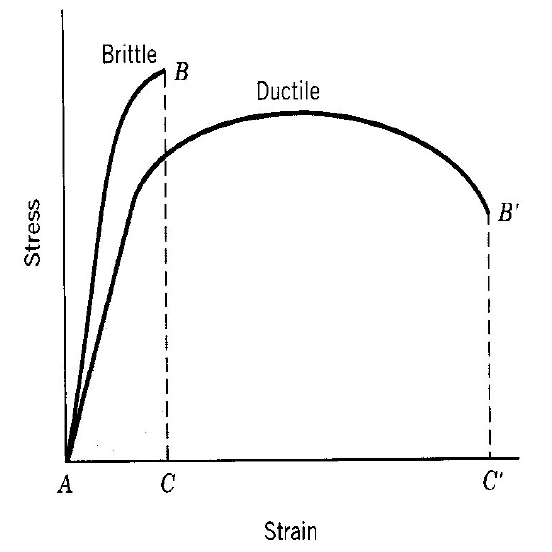
\includegraphics[width = 0.4\textwidth]{ProvaTrazione}} \quad
\subfloat[][\emph{Grafico prova di trazione con snervamento discontinuo}\label{fig:trazioneDiscontinua}]{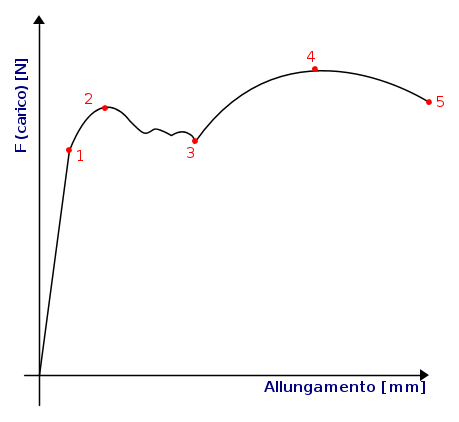
\includegraphics[width = 0.4\textwidth]{TrazioneDiscontinua}}
\caption{Prove di trazione}\label{fig:Trazione}
\end{figure}
Se si osserva il grafico della prova di trazione \ref{fig:TrazioneContinua}
si osservano 2 particolari zone: comportamento elastico del materiale e comportamento plastico.
Ricordando l'equazione constitutiva del materiale ovvero
\begin{equation}
\sigma = K \epsilon ^n
\label{eq:Cost}
\end{equation}
Dove i termini di \ref{eq:Cost} sono:\\
\begin{tabular}{cl}
$\sigma$ & tensione [MPa]\\
$K$ & coefficiente di resistenza\\
$\epsilon$ & fattore di incrudimento\\
$n$ & Sensibilità alla velocità di incrudimento\\
\end{tabular}
\\
Dalla \ref{eq:Cost} si può intuire che il il fattore $K$ lo si volgia particolarmente grande al fine di garantire un'alta resistenza allo snervamento.
La stizione si manifesterà su una sezione "più debole" (impurità, vuoti, ecc\dots), da cui avrà luogo una deformazione della sezione stessa. Dunque sulla sezione si manifesterà incrudimento dovuto proprio alla trasformazione.
L'incrudimento renderà la sezione molto più dura rispetto alle circostanti. Perciò si può dimostrare come il valore per cui la strizione si stabilizza è proprio pari al coefficiente $n$.
Sotto queste ipotesi allora vale:
\begin{equation}
\epsilon = n
\label{eq:StrizzCost}
\end{equation}
In generale si preferisce utilizzare materiali con coefficiente $n$ molto alto: per cui il materiale 
si deforma molto prima della strizione. Dunque è più \textbf{duttile}.

\subsection{Snervamento discontinuo}
Lo snervamento discontinuo è tipico dei metalli che hanno basso valore interstiziale.
Tipicamente, a fine lavorazione di tali metalli si presentano le \textbf{bande di Lüder}. Di fatto non costituiscono un difetto tecnologico, piuttosto puramente estetico. Siccome le lamiere vengono utilizzate anche per coperture, tali bande fanno sembrare il prodotto più scadente (Anche se di fatto non lo è).
Il grafico \ref{fig:trazioneDiscontinua} rappresenta il comportamento di un materiale a snervamento discontinuo.

\section{Tessitura e anisotropia}
La tessitura è la descrizione della presentazione, sia estetica che prestazionale, del materiale
Logicamente dipende direttamente dai grani cristallini presenti nel materiale.

Quando questi si presentano in forma allungata (es. post laminazione), portano 
a delle differenze dal punt odi vista meccanico-fisico del prodotto. 
Portando \textbf{anisotropia}.
Già si sa che i piani preferenziali di scorrimento sono quelli ad alte densità atomica
e, nel caso non ce ne siano a sufficienza, il materiale tenderà a costituirne di nuovi%
\footnote{Si vedrà anche in seguito che la questione dei piani di scorrimento è cruciale per la qualità del materiale}.

\subsection{Proprietà modificate}
Ricordando i principali termini di descrizione delle proprietà meccanico-fisiche dei metalli:\\
\begin{tabular}{cl}
$Y$ & Densità di snervamento\\
$T_S$& Resistenza meccanica\\
\end{tabular}
\\
Inoltre anche altre proprietà, non necessariamente meccaniche, vengono modificate da eventuali lavorazioni a freddo.
Allora: considerando una lamiera lavorata a freddo vale:
\begin{equation}
\epsilon_1 + \epsilon_2 + \epsilon_3 = 0 \underbrace{\rightarrow}_{\text{per lamiere}}
\epsilon_l + \epsilon_w + \epsilon_t = 0 
\label{eqn:DefCost}
\end{equation}
La \ref{eqn:DefCost} definisce la \emph{costanza della deformazione del volume principale}.
Si considerano pedici diversi da quelli classici per un volume massivo in quanto stiamo considerando una lamiera, percui i nuovi pedici indicano:\\
\begin{tabular}{cl}
$l$ & \textit{lenght}\\
$w$ & \textit{width}\\
$t$ & \textit{thickness}\\
\end{tabular}
\\
Si ricordano, inoltre, le deformazioni per le principali grandezze:
\begin{equation}
\epsilon_w = \ln{\frac{w_1}{w_0}} \qquad \epsilon_t = \ln{\frac{h_1}{h_0}}
\label{eqn:DefPrinc}
\end{equation}
Dove $w_1$ e $h_1$ sono le misurazioni dopo la prova di trazione, mentre $w_0$ e $h_0$ sono i valori iniziali.
A partire dai termini sopraelencati, si può definire il parametro $r$ definito come nella \ref{eqn:r}.
\begin{equation}
r = \frac{\epsilon_w}{\epsilon_t}
\label{eqn:r}
\end{equation}
Non ha un nome specifico, nonostante rappresenti la quantità di deformazione che una lamiera subisce se sottoposta a trazione.
In particolare, le due deformazioni considerate sono quella in termini di spessore e quella in larghezza.
Se il materiale avesse:
\begin{equation}
r = 1
\end{equation}
potrebbe essere considerato isotropo. Più correttamente si definiscono \textbf{isotropi} tutti quei materiali per cui vale la \ref{eqn:DefIsotropo}.
\begin{equation}
r_0 = r_{45} = r_{90} = 1
\label{eqn:DefIsotropo}
\end{equation}
dove i fattori $r$ sono il rapporto tra le deformazioni come sopra però ponendo la trazione con angolo tanto quando indicato dal pedice:\\
\begin{tabular}{cl}
$r_0$ & Direzione laminazione\\
$r_{45}$ & Direzione intermedia\\
$r_{90}$ & Direzione ortogonale
\end{tabular}
\\
Altrimenti il materiale è semplicemente \textbf{anisotropo}.
L'anisotropia può essere un problema in termini di lavorazione di una lamiera: si prenda come esempio il caso della realizzazione di un contenitore per estrusione. Se il materiale fosse isotropo allora la deformazione avverrebbe in maniera uniforme su tutta la lamiera.
Se, invece, il materiale è anisotropo, la deformazione diversificata produce variabilità sul bordo del prodotto. Successivamente sarebbe necessario un operazione di \textit{trimming} per eliminare il materiale in eccesso.
L'anisotropia si può verificare in diverse forme.
\begin{description}
\item[$r_0 = r_{45} = r_{90} \lessgtr 1$] allora si parla di \textbf{Anisotropia normale} alla superficie della lamiera. Se ne può misurare il valore tramite:
\begin{equation}
r_m = \overline{r} = \frac{r_0 + r_{90} + 2 * r_{45}}{4}
\label{eqn:MisAnisotropia}
\end{equation}
\item[$r_0 \neq r_{45} \neq r_{90}$] allora si parla di \textbf{compresenza di anisotropia planare e normale} da cui si può ottenere una misura
\begin{equation}
\Delta r = \frac{r_0 + r_{90} - 2 * r_{45}}{2}
\label{eqn:MisPlanare}
\end{equation}
\end{description}
In generale l'anisotropia si verifica quando, durante la laminazione, i reticoli cristallini si muovono per garantire i piani di scorrimento.
Ora si vuole dare una rapida visione delle principale strutture cristallini nei materiali.

\subsubsection{Reticolo esagonale compatto}
I piani di scorrimento si trovano sulle superfici di base del prisma compatto.
Si definisce \textit{compatto} perché il rapporto tra l'altezza del prisma e la lunghezza di un lato di base, ovvero $c/a$ considerando i riferimenti della figura \ref{fig:EsaComp}.
\begin{figure}
\centering
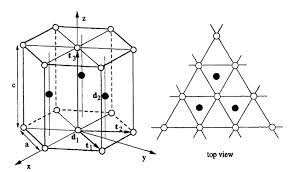
\includegraphics[width = 0.8\textwidth]{Esagono1}
\caption{Esagonale compatto}
\label{fig:EsaComp}
\end{figure}
Si osserva che il rapporto \ref{eqn:r} per materiali con reticolo cristallino \eng{High c/}a è prossimo a a 0:
\begin{equation}
r_{\text{High c/a}} = \frac{\epsilon_w}{\epsilon_t} \longrightarrow 0
\label{eqn:HighC_AR}
\end{equation}
Nella maggior parte dei casi si vuole un rapporto $r$ il più alto possibile. Così ché la deformazione della lamiera interessi la larghezza piuttosto dello spessore. Altrimenti potrebbero sorgere problemi sulla rigidità della lamiera anche senza eseguire alcuna lavorazione.
Potremmo allora dire che:
\begin{description}
\item[$n$] indichi il ritardo nella deformazione (sensibilità alla deformazione)
\item[$r$] indichi che tipo di deformazione si avrà. 
\end{description} 

Nel caso di materiali ad esagonale compatto ma con rapporto $c/a$ basso si osserva:
\begin{equation}
r_{\text{Low c/a}} \longrightarrow \infty 
\end{equation}
Ad esempio per guadagnare duttilità nel titanio (Ti) si effettuano lavorazioni a caldo.

\subsubsection{Reticolo cubico}
\begin{figure}
\centering
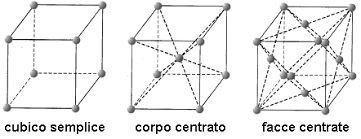
\includegraphics[width = \textwidth]{Cubico}
\caption{Reticoli cubici}
\label{fig:Cubici}
\end{figure}
Per i metalli cristallizzanti a \ac{CFC} si osserva un valore di $r\approx 0.4 \div 0.8$.
Mentre per i metalli a \ac{CCC} si osservano valori di $r \approx 1$.

\section{Effetti delle lavorazioni a freddo}
Come già accennato in precedenza, le lavorazioni a freddo permettono di ottenere da un materiale metallico sì la deformazione voluta. In più si garantisce al materiale maggiore durezza.
Ciò è dovuto allo scorrimento delle dislocazioni, durante la lavorazione del materiale, che vengono bloccate dal bordo del grano cristallino.
Di contro bisogna tenere a mente che una maggiore durezza impone una minore duttilità, considerazione che serve nel caso la lamiere debba subire diverse lavorazioni prima di divenire prodotto finito.
\missingfigure{Da aggiungere il grafico tridimensionale sulla deformazione a freddo.}
\missingfigure{Aggiungere proiezioni del grafico precedente in due dimensioni.}

Dunque le lavorazioni a freddo hanno diversi vantaggi e svantaggi come descritto nella tabella \ref{tab:VantSvantFreddo}.

\begin{table}
\centering
\caption{Vantaggi e svantaggi delle lavorazioni a freddo}
\label{tab:VantSvantFreddo}
\begin{tabularx}{\textwidth}{XX}
\toprule
\textcolor{UnifeDark}{\textbf{Vantaggi}} & \textcolor{UnifeDark}{\textbf{Svantaggi}}\\
\midrule
Metodo economico per indurire il materiale &
Pressione sugli stampi più alti\\
Il prodotto è quasi finito finite le lavorazioni (in genere) &
Bisogna trovare un compromesso tra durezza desiderata e consumo delle attrezzature\\
\bottomrule
\end{tabularx}
\end{table}

Per ovviare ad alcuni problemi evidenziati alla tabella \ref{tab:VantSvantFreddo}, si può pensare di ricorrere a ricotture parziali o complete.
Alcuni esempi sono riportati alle figure \ref{fig:RsRicottura}

In particolare:
\begin{description}
\item[Lavorazione a freddo $T < 0.3 T_m$] evidenzia un chiaro incrudimento del materiale, che ne risulterà indurito.
\item[Ricotture di distensione $0.3T_m < T < 0.5 T_m$] Permette una ridistribuzione delle dislocazioni ma senza ricristallizzazione
\item[Ricottura di ricristallizzazione $T > 0.5 T_m$] Non è scontata la ricristallizzazione ma si ha una distensione dei grani, annullando eventuali lavorazioni a freddo precedenti.
\end{description}
Nonostante ciò le ricotture possono essere molto interessanti per le caratteristiche meccaniche dei materiali metallici.
Ipotizzando di voler raggiungere un determinato obbiettivo di duttilità del materiale. Si può raggiungere tale obbiettivo semplicemente lavorando il materiale a freddo, dando una certa deformazione al pezzo.
Sappiamo che così il pezzo sarà più indurito di conseguenza.
C'è un ulteriore modo: se si incrudisce di più rispetto al obbiettivo, attraverso una deformazione maggiore di quella desiderata, si può pensare di sfruttare una ricottura di distensione per ritornare al livello di duttilità richiesto ma garantendo un livello di durezza maggiore rispetto alla sola lavorazione a freddo. In genere vale anche il viceversa. 
Tale metodo viene chiamato \textit{forte incrudimento con ricottura parziale}.
Alla figura \ref{fig:Ricot} è graficato l'andamento delle tensioni di snervamento e rottura dopo una ricottura completa. Si osserva che vengono perse completamente le caratteristiche meccaniche guadagnate tramite incrudimento per lavorazione a freddo.
Alla figura \ref{fig:RicotRs} viene mostrato il processo per ottenere una determinata tensione di snervamento dopo forte incrudimento. 

\begin{figure}
\centering
\subfloat[][\emph{Duttilità, snervamento e rottura dopo ricottura}\label{fig:Ricot}]%
{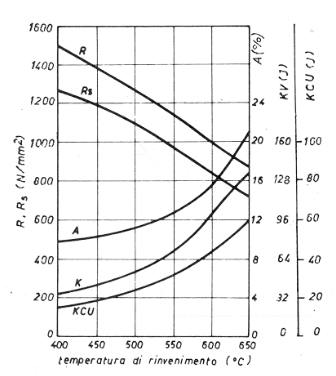
\includegraphics[width = 0.4\textwidth]{Rinvenimento}}\quad
\subfloat[][\emph{Durata ricottura in base allo snervamento richiesto}\label{fig:RicotRs}]%
{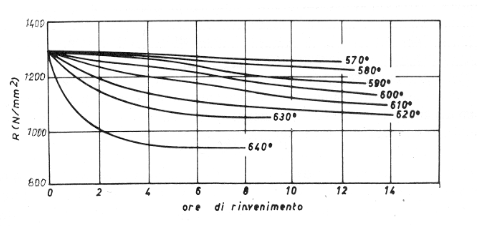
\includegraphics[width = 0.4\textwidth]{CotturaRinvenimento}}
\caption{Andamenti tipici di un acciaio dopo ricottura}\label{fig:RsRicottura}
\end{figure}

Ipotizzando una ricottura completa, ovvero portando il materiale a una temperatura $T > 0.5\:T_m$, si può avere ricristallizzazione del metallo che porta grani a dimensioni maggiori. Bisogna anche tenere a mente l'influenza del tempo su questi processi di ricottura.

\subsection{Effetti della velocità di deformazione}
Come visto nell'equazione costitutiva \ref{eqn:DefCost}, il materiale viene univocamente definito tramite tale equazione. In realtà è necessario "mettere in relazione" anche il tempo. Considerando l'equazione costitutiva per lavorazione a caldo:
\begin{equation}
\sigma_f = C \cdot \dot{\epsilon}^m
\label{eqn:CostCaldo}
\end{equation}
Da cui si può osservare che se la temperatura aumenta allora $C$ diminuisce e contemporaneamente $m$ cresce. Infatti:
\begin{description}
\item[$C$] è il coefficiente di resistenza alla temperatura del materiale;
\item[$m$] è l'indice di sensibilità alla velocità di deformazione;
\item[$\dot{\epsilon}$] è la velocità di deformazione descritta come $V/h$
\end{description}
Con una strizione diffusa, l'incrudimento è diffuso su tutto il provino. E, come si era visto anche in precedenza, ciò migliora le caratteristiche meccaniche. Se invece, la strizione è localizzata rischia di indebolire il materiale.
Il fatto che sia locale indica che il materiale in quel punto è più debole e può rompersi più facilmente.

\begin{definition}{Considerazione}{*}
In generale si privilegiano metalli che abbiano alta sensibilità al incrudimento e maggiore sensibilità alla velocità di strizionamento.
\end{definition}


Si vogliono ricordare i valori per cui $m$ porta ad un determinato comportamento il materiale:
\begin{description}
\item[$-0.05 < m < 0.05$] \eng{Cold working}
\item[$0.05 < m < 0.3$] \eng{Hot working}
\item[$0.3 < m < 0.7$] \eng{Superplasicity}%
\footnote{Valori di deformazione tipici delle lavorazioni con materiali plastici}
\item[$m > 1$] \eng{Newtonian fluid}
\end{description}

\section{Limiti di formabilità delle lamiere}
\begin{enumerate}
\item Manifestazione di strizioni localizzate.
\item Con strizione diffusa, prima della rottura.
\item Generazione delle bande di L\"uder
\item Generazione della superficie a buccia d'arancia
\end{enumerate}
A parte le prime due che portano a conseguenze meccaniche per cui la lamiera effettivamente non può più essere vendute o utilizzate per la produzione.
La terza ha una motivazione puramente estetica: siccome le lamiere possono essere utilizzate come copertura, tale superficie può essere problematica. Non lo è dal punto di vista meccanico-fisico.
La superficie a buccia d'arancia anch'essa non influisce sulle prestazione meccaniche del prodotto%
\footnote{C'è da dire che una maggiore porosità superficiale potrebbe stimolare la generazione di cricche in alcune lavorazioni.}.
La formazione è dovuta alla rotazione dei grani cristallini durante eventuali lavorazioni.
La soluzione è quella di sfruttare, per le lamiere in particolare, materiali a grana fine.

\subsection{Come mai le lamiere?}
Le lamiere vengono largamente impiegate per la produzione di oggetti metallici, e le tecniche che verranno trattate in questo corso volgono a a sfruttare tale prodotti in larga scala.
Alcuni motivi dell'espansione del loro impiego sono:
\begin{itemize}
\item A parità di prodotto, un oggetto pieno e uno ricavato tramite lavorazione di lamiera risulta più pesante.
\item La laminazione è una lavorazione molto efficiente: si producono tanti pezzi in poco tempo e con minore energia.
\item La laminazione permette di raggiungere risultati molto accurati (in termini di spessori e qualità del laminato) con poche risorse, dunque ad un costo molto basso.
\item La lamiera è un prodotto "quasi" pronto all'uso.
\end{itemize}

\section{Materiali per lamiere}
I materiali che in industria vengono più comunemente utilizzati per lamiere sono ad esempio:
\begin{itemize}
\item Acciai, dolci + inossidabili
\item Leghe di allumino
\item Ottoni
\item Bronzi
\item Rame
\item Magnesio
\item Titanio
\end{itemize}
Sebbene la maggior parte dei prodotti in lamiera siano lavorati a freddo, ci sono alcuni materiali che necessitano di lavorazioni a caldo.
In particolare alla figura \ref{fig:LavCaldo}, si presentano i motivi per cui sia necessaria la lavorazione a caldo

\begin{figure}
\centering
\usetikzlibrary{trees}
\begin{tikzpicture}[
sibling distance = 10em,
every node/.style={rectangle, rounded corners, draw, align=center}]
\node[top color=UnifeLight]{Lavorazioni a caldo}
	child{node[top color=UnifeDark, bottom color=UnifeDark!50, white]{Esagonale\\compatto}
		child{node[top color=UnifeDark!50, bottom color=UnifeDark!50, white]{Maggiore\\duttilità}}
		child{node[top color=UnifeDark!50, bottom color=UnifeDark!50, white]{Si spera in\\un cambio\\di reticolo}}}
	child{node[top color=UnifeDark, bottom color=UnifeDark!50, white]{Superplasticità}}
	child{node[top color=UnifeDark, bottom color=UnifeDark!50, white]{Forze troppo\\alte}};
\end{tikzpicture}
\caption{Motivazioni delle lavorazioni a caldo}
\label{fig:LavCaldo}
\end{figure}
Ora si vedranno nel dettaglio tutte le caratteristiche e motivazioni per cui viene scelta una determinata categoria di materiali.

\subsection{Acciai}
In genere si preferiscono acciai che abbiano un tenore di carbonio minore del 0.15\%, ovvero gli acciai dolci.
Inoltre, bisogna includere gli acciai inossidabili: sia per motivi di mercato, che necessità operative dei prodotti finali.
Essendo una gamma decisamente ampia di materiali, le lavorazioni possibili sono molteplici:
\begin{description}
\item[lavorazioni a caldo] non vengono sfruttate troppo per gli acciai in quanto si preferisce mantenere l'incrudimento ottenuto tramite la lavorazione a freddo. Anche se si impiega per:
	\begin{itemize}
	\item Ottenere maggiore duttilità per il materiale.
	\item Quando le forze in gioco sono eccessive è opportuno aumentare la duttilità grazie ad 
	una maggiore temperatura.
	\end{itemize}
	Si rischia di incorrere in:
	\begin{itemize}
	\item Finiture peggiori.
	\item Maggiore rugosità da cui derivano pure caratteristiche meccaniche peggiori.
	\item Non si ottiene incrudimento. 
	\end{itemize}
\item[Lavorazioni a freddo] In industria vengono sfruttate molto più volentieri per via:
	\begin{itemize}
	\item Migliori tolleranze geometriche ottenibili.
	\item Migliore finitura superficiale,
	\item Migliori prestazioni meccaniche a parità mi materiale usato.
	\end{itemize}
\end{description}

  %Introduzione e lavorazioni su lamiera
\part{Sitenrizzazione}
\cleardoublepage \chapter{Sinterizzazione}\label{chp:Sinterizzazione}
Permette di realizzare oggetti a partire da polveri di un
materiale.

\begin{quote}
\emph{Perché sfruttare la sinterizzazione?}
\end{quote}

I motivi sono molteplici e possono essere:
\begin{itemize}
\item controllo accurato della struttura richiesta;
\item controllo della composizione chimica;
\item formabilità;
\item Quando non si vogliono macrosegregazioni;
\item realizzare dei componenti in materiali con temperatura di 
fusione particolarmente alta.
\end{itemize}

A differenza di altre lavorazioni è necessario parametrizzare la 
forma delle polveri, in quanto da quei parametri si possono ottenere 
le caratteristiche meccaniche del lavorato finale.
Inoltre la forma della polvere può essere determinante sulla
lavorazione.

Per i prodotti lavorati in sinterizzazione si parla di \eng{Net-
Shape}: ovvero, la lavorazione porta dei semilavorati già molto 
vicini alla forma finale di vendita del prodotto.
Ciò permette di usare tutto il materiale, senza avere sprechi dovuti
a delle lavorazioni che per ottenere la forma finale, devono 
eliminare parte di esso.

Data la lavorazione è possibile controllare la porosità del prodotto
come si vedrà successivamente.
In generale non si ottengono particolari caratteristiche meccaniche
anche se alle volte si possono ottenere delle caratteristiche 
migliori di altre lavorazioni già viste.

Bisogna prestare attenzione al discorso della porosità: troppa
porosità residua può essere punto di fragilità del materiale portando
alla formazione di cricche.
In più non sono facili da lavorare in post-produzione. Quindi il 
processo di produzione deve essere \eng{near net-shape} il più
possibile.

\section{La lavorazione}
Alla figura \ref{fig:ProcSint} sono riportati i principali
possibili processi per le lavorazioni di sinterizzazione.

\begin{figure}
\centering
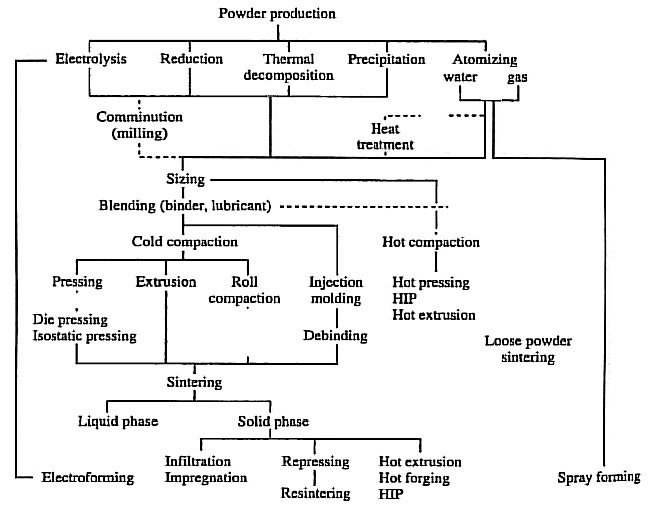
\includegraphics[width = \textwidth]{ProcSint}
\caption{Processi di produzione in sinterizzazione}
\label{fig:ProcSint}
\end{figure}

In generale il processo di sinterizzazione deve passare attraverso 
tre principali processi:

\begin{center}
\smartdiagramset{%
sequence item uniform color = UniFeLight!50,
sequence item width = 0.3\textwidth,
back arrow disabled=true}
\smartdiagram[sequence diagram]{Produzione Polveri, Compattazione, Sinterizzazione}
\end{center}

Sarà anche la la sequenza delle trattazioni successive.

\subsection{Produzione delle polveri}
  %Sinterizzazione
\part{Asportazione di truciolo}
\cleardoublepage \chapter{Lavorazioni per asportazione di truciolo}\label{chp:AsportaTruciolo}
Il principio di funzionamento delle lavorazioni per asportazione di truciolo è
differente da quanto visto fin ora.
Nelle lavorazioni per deformazione plastica si avevano delle deformazioni lente.
\emph{"Per cui il materiale aveva il tempo di adattarsi"}.
Per l'asportazione di truciolo così non può essere. Infatti si suppone che il
materiale venga rotto, tra l'altro il più rigidamente possibile.
Dunque le deformazioni richieste devono essere a più alta velocità.
Ciò però crea delle problematiche non indifferenti:
\begin{itemize}
\item deformazioni veloci non sono rappresentabili tramite prove classiche.
\item Si rende necessario idealizzare il processo e man mano aggiungere ipotesi più realistiche.
\end{itemize}

\section{Introduzione}
Nelle lavorazioni viste fin ora si portava il materiale a deformazione, anche per la tranciatura
nel momento in cui il materiale subiva una deformazione critica fino all'innesco di cricche da cui poi
avveniva la separazione del materiale.
Per l'asportazione del truciolo non può essere così: la deformazione avviene in tempi molto più rapidi,
per cui il materiale ha comportamenti differenti da quelli visti in precedenza.
Inoltre, considerando il materiale di scarto, per le lavorazioni a deformazione si può recuperare ed 
eventualmente riciclare.
Per le lavorazioni ad asportazione la cosa è molto più complicata e difficile.
Il valore del truciolo è pressoché nullo e il suo recupero può essere complicato 
per via delle molteplici varietà di materiale che possono subire tali lavorazioni.
Alla tabella \ref{examp:VantSvant} sono riportati alcuni vantaggi e svantaggi di tali lavorazioni.

\begin{example}{Vantaggi e Svantaggi}
\centering
\begin{tabularx}{\textwidth}{XX}
\toprule
\textbf{Vantaggi} & \textbf{Svantaggi}\\
\midrule
Si possono ottenere tolleranze migliori & Tempo ciclo molto più lento\\
\midrule
Buona finitura superficiale & Scarti di materiale non recuperabili\\
\midrule
\multicolumn{2}{c}{Adatti alla lavorazione di pezzi unici}\\
\midrule
Costo macchina relativamente basso & Spesso è richiesta alta lavorazione manuale\\
\bottomrule
\end{tabularx}
\label{examp:VantSvant}
\end{example}

In industria si sta cercando di eliminare queste lavorazioni per via del tempo ciclo molto elevato.
Sebbene, in abito artigianale stiano avendo un forte sviluppo, sia in termini di automazione,
dunque di tecnologia a bordo macchina; sia di lavorazioni permesse dalle macchine.
Altro grande punto a favore di tali lavorazioni è sicuramente l'adattabilità per 
qualsiasi materiale.

In industria, vengono relegate ad operazioni di finitura del prodotto, dove con una
singola passata si cerca di completare il prodotto e metterlo sul mercato.
Per l'artigianato invece si ha un utilizzo più intensivo, dove con una passata si cerca 
di ottimizzare la quantità di materiale asportato.

Come punto di partenza è utile considerare applicazioni in cui il processo sia completamente
idealizzato.

\section{Taglio ortogonale ideale}
Alla figura \ref{fig:TaglioOrto} sono rappresentati degli esempi di taglio ortogonale.

\begin{figure}
\centering
\subfloat[][\emph{Visualizzazione del taglio ortogonale}\label{fig:TaglioOrto}]
{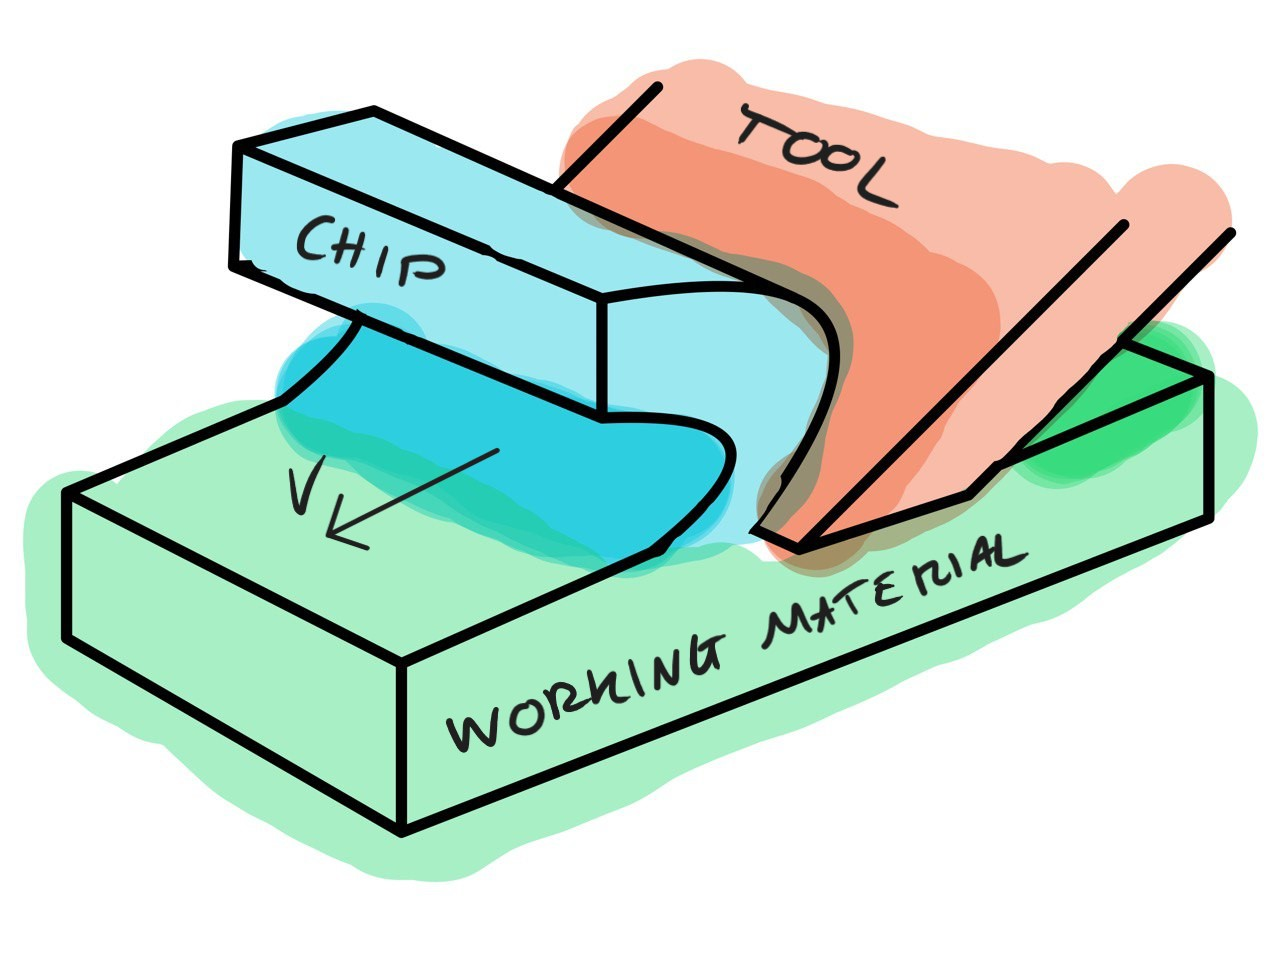
\includegraphics[width = 0.8\textwidth]{TaglioOrto}}\\
\subfloat[][\emph{Parametri del taglio ortogonale}\label{fig:TaglioOrtoParam}]
{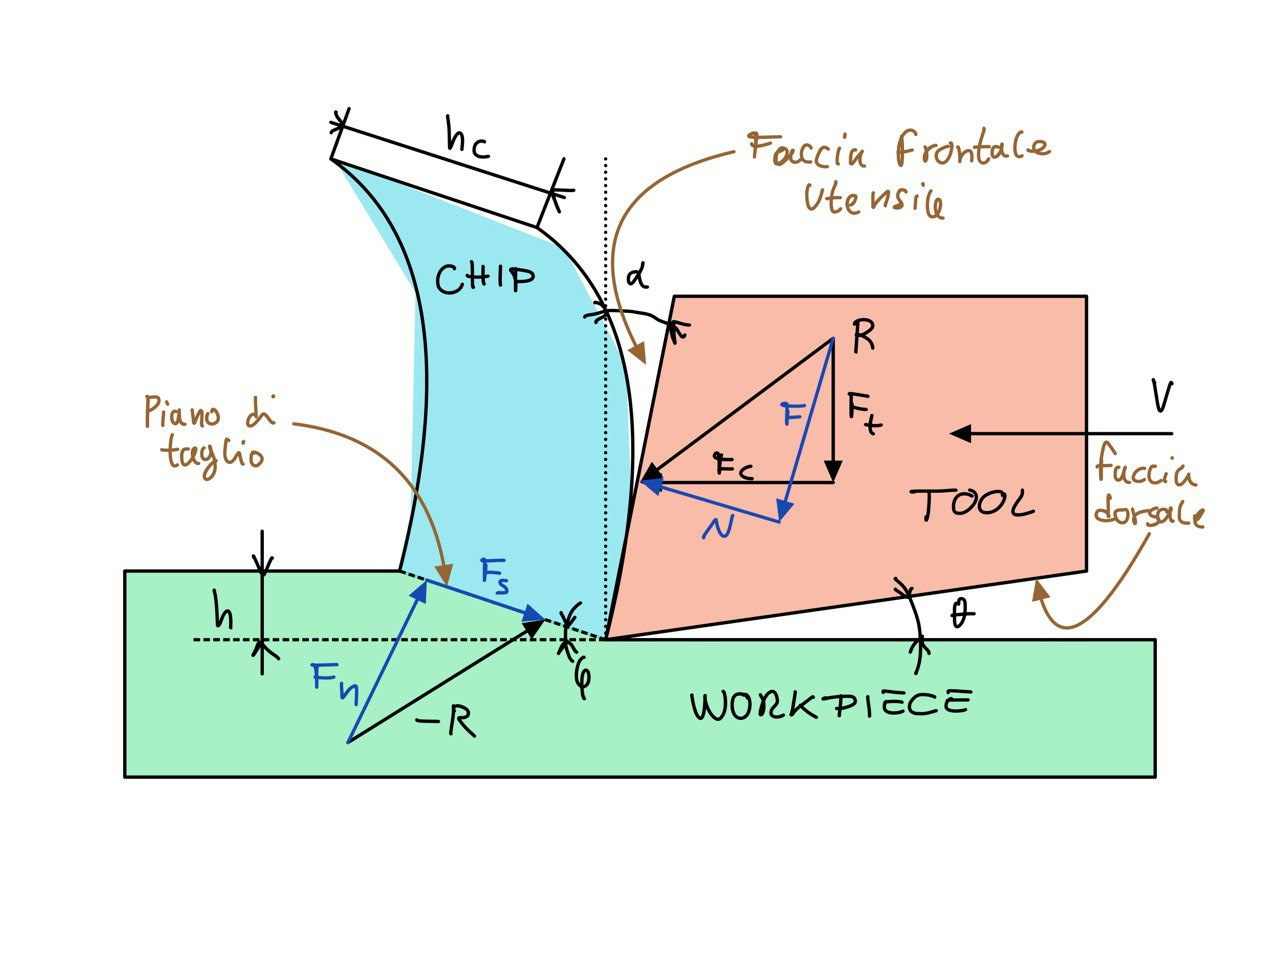
\includegraphics[width=0.7\textwidth]{TaglioOrtoScheme}}
\caption{Taglio Ortogonale}\label{fig:TaglioOrto}
\end{figure}
Si dice che il taglio è ortogonale quando la lama dell'utensile è ortogonale alla direzione della velocità di taglio.
Allora si possono definire diversi parametri come riportato nella definizione \ref{def:ParamTaglioOrto}.

\begin{definition}{Parametri del taglio ortogonale}{pramTaglioOrto}
\begin{description}
\item[$\alpha$] Angolo di spoglia superiore o frontale. Da cui
	\begin{description}
	\item[Se $\alpha > 0$] allora si dice che l'utensile ha angolo acuto,
	\item[Se $\alpha < 0$] allora si dice che l'utensile ha angolo ottuso.
	\end{description}
\item[$\theta$] Angolo di spoglia inferiore
\item[$\phi$] Angolo di taglio
\item[$h$] Spessore di taglio indeformato
\item[$h_c$] Spessore del truciolo
\end{description}
\label{def:ParamTaglioOrto}
\end{definition}

Come ipotesi ideale, si considererà che tutta la deformazione del materiale avverrà
solamente sul piano di taglio.
Allora, dai parametri del taglio ortogonale si possono ottenere:
\begin{equation}
r_c = \frac{h}{h_c} = \frac{l_c}{l} := \text{Rapporto di taglio}
\end{equation}
Dove:\\
\begin{tabular}{cl}
$l_c$ & è la lunghezza del truciolo\\
$l$ & è la lunghezza del taglio\\
\end{tabular}
\\
Mentre:
\begin{equation}
F = K \cdot A
\end{equation}
ovvero, la forza necessaria a tagliare il pezzo sarà proporzionale all'area $A$ del piano di taglio 
dovuta dalla lunghezza del piano stesso per la profondità del pezzo in senso ortogonale alla 
figura \ref{fig:TaglioOrtoParam}; in più sarà proporzionale alla pressione $K$ esercitata dall'utensile sul pezzo
Inoltre, si può intuire che: per abbassare l'intensità della forza complessiva per il taglio
sarebbe opportuno aumentare $\phi$, così da limitare l'estensione del piano di taglio e di 
conseguenza la sua area.
Si può ottenere una stima dell'angolo di taglio tramite
\begin{equation}
\tan\phi = \frac{r_c \cos\alpha}{1-r_c\sin\alpha}
\end{equation}
considerando che il rapporto di taglio lo si può misurare abbastanza facilmente dato che:
lo spessore di taglio lo si decide in base alla lavorazione da effettuare, mentre lo
spessore del truciolo lo si può misurare abbastanza facilmente.
Dunque è evidente che l'angolo $\alpha$ lo si vuole molto grande, in modo da generare piani
di taglio molto piccoli: garantendo la necessità di applicare una forza minore.

Risulta utile prestare attenzione alla successiva considerazione.
Il valore di deformazione che si raggiunge con le lavorazioni per asportazione di truciolo
è nettamente più alte che non le deformazioni per lavorazioni tramite deformazione.
Giusto per dare un'idea dell'ordine di grandezza:
\begin{equation}
\dot{\gamma} = \frac{v_s}{d} = \frac{\cos\alpha}{\cos\left(\phi - \alpha\right)} \frac{v}{d} \left[\unit{\s^{-1}}\right]
\end{equation}
nella tecnica, si osservano i seguenti valori:
\begin{description}
\item[Lavorazione per deformazione] $\approx 1 \div 10 \left[\unit{\s^{-1}}\right]$
\item[Lavorazione per asportazione] $\approx 1000 \left[\unit{\s^{-1}}\right]$
\end{description}

\subsection{Fattore di attrito}
Sappiamo che il fattore di attrito ricopre importante ruolo per quanto riguarda questo tipo
di lavorazioni. Ci si deve prestare attenzione.

\begin{equation}
\mu = \frac{\tau_i}{p}
\label{eqn:FattoreAttritoIndef}
\end{equation}
Di base, questa sarebbe la definizione principale di fattore di attrito.
Si nota che passata la tensione tangenziale di Von Misess, 
l'attrito tende a calare, nonostante nell'equazione non sia previsto tale 
comportamento.
Ciò è dovuto al fatto che per calcolare il fattore di attrito si considera un materiale
indeformabile, quando nella realtà del taglio ortogonale, non può essere.
Dunque il materiale sarà \textbf{indeformabile} fino alla tensione di Von Misess, 
passata quella bisogna considerarlo \textbf{deformabile}.
Perciò l'equazione \eqref{eqn:FattoreAttritoIndef} non descrive completamente il comportamento.
Si è sviluppato un \texttt{fattore di attrito} adatto a tale fenomeno:
\begin{equation}
m = \frac{\tau_i}{K}
\label{eqn:FattoreAttritoDef}
\end{equation}
Dove $K$ è la tensione tangenziale all'interfaccia truciolo-utensile.
Nella pratica viene preferito il fattore descritto dalla \eqref{eqn:FattoreAttritoDef} 
perché più facile da calcolare. Oltre al fatto che permette di descrivere correttamente
il fenomeno dello \eng{sticking}.

\begin{definition}{Sticking}{*}
Fenomeno di aderenza tra il truciolo e l'utensile. 
\end{definition}

\subsection{Valutazione delle forze}
Per la valutazione delle forze messe in gioco per tale lavorazione si considereranno
i tre attori separatamente e man mano sovrapponendone gli effetti.

\begin{figure}
\centering
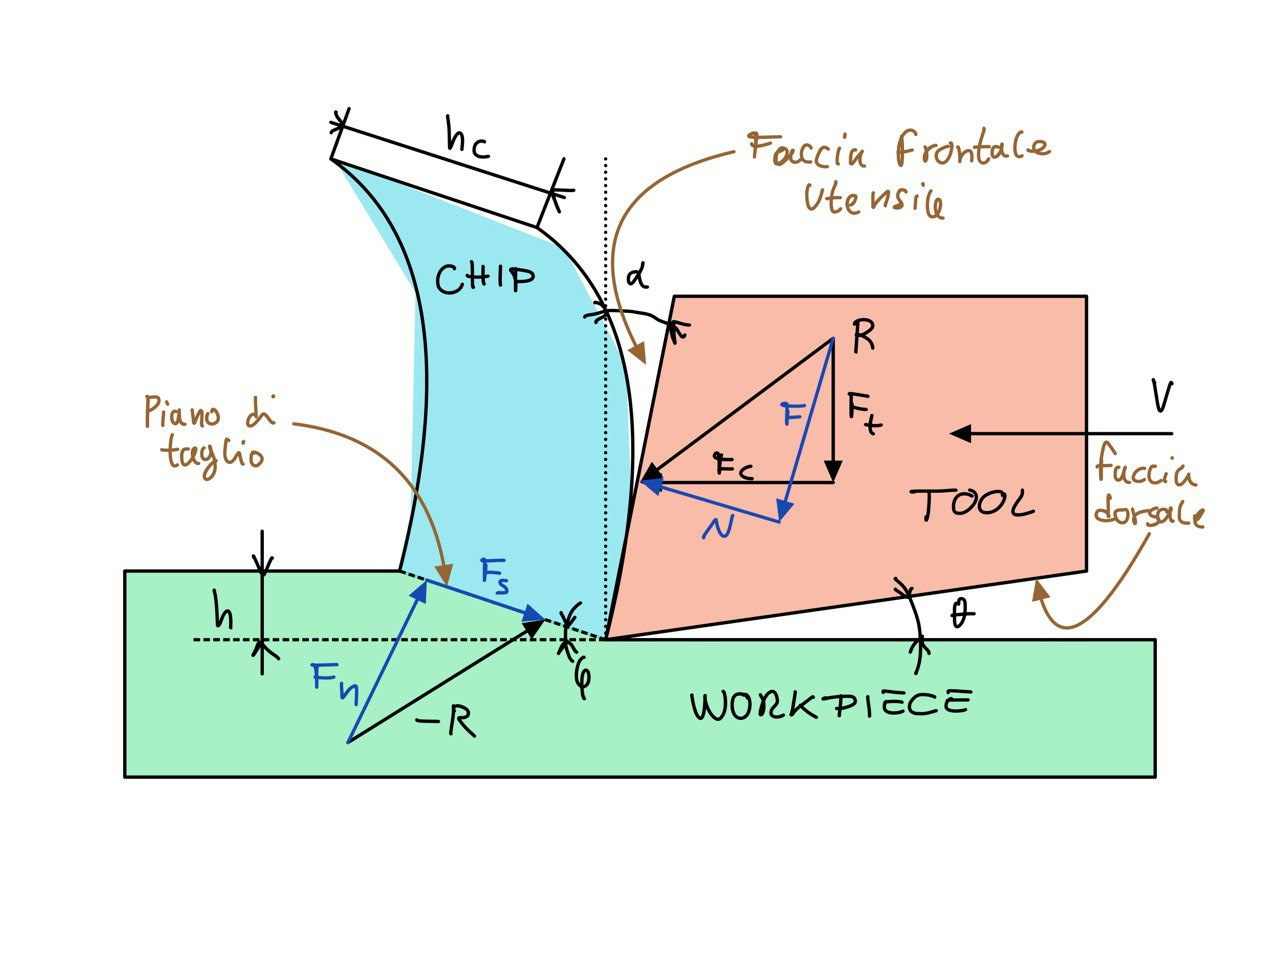
\includegraphics[width = \textwidth]{TaglioOrtoScheme}
\caption{Scomposizione delle forze per il taglio ortogonale}
\label{fig:TaglioOrtoForces}
\end{figure}

\subsubsection*{Porta utensile}
Considerando la scomposizione delle forze della figura \ref{fig:TaglioOrtoForces}.
Al porta utensile si può, operativamente, applicare una cella di carico per 
valutare la risultate applicata. Celle di carico più moderne possono eventualmente
valutare già le componenti di tale risultante.
allora possiamo ottenere i moduli delle forze:
\begin{equation}
\begin{cases}
F_c = R \cos(\alpha + \psi) &\text{Forza di taglio}\\
F_t = R \sin(\alpha + \psi) &\text{Forza di spinta dell'utensile}
\end{cases}
\end{equation}
Si possono definire ulteriori scomposizioni di forze: se prima la scomposizione
avveniva su proiezioni degli assi di riferimento rispetto al pezzo lavorato; ora si 
possono definire delle scomposizioni rispetto all'utensile.

\subsubsection*{Utensile}
Sempre in riferimento alla figura \ref{fig:TaglioOrtoForces}.
\begin{equation}
\begin{cases}
N = F_c \cos\alpha - F_t\sin\alpha\\
F = F_c \sin\alpha - F_t\cos\alpha
\end{cases}
\end{equation}
L'angolo relativo tra $R$ e $N$ viene indicato con $\beta$ e viene definito come 
\textbf{angolo d'attrito sulla faccia dell'utensile}. Vale:
\begin{equation}
\beta = \frac{F}{N} \approx \mu
\label{eqn:AngAttrito}
\end{equation}
Notare che $\beta$ è una sottospecie di coefficiente di attrito, infatti dipende
proprio da quest'ultimo.

\subsubsection*{Pezzo lavorato}
Lato pezzo lavorato si può vedere la totalità delle forze in gioco.
in particolare si devono evidenziare le forze:
\begin{description}
\item[$F_n$] risulta essere un contributo idrostatico per il materiale, dunque ne aumenta la 
duttilità. Aspetto che rende il taglio più difficoltoso. 
Ciò si risolve aumentando l'angolo del piano di taglio $\phi$ che si vedrà successivamente.
\item[$F_s$] è la vera e propria forza resistente al taglio. Si sviluppa come relazione della 
pressione di taglio resistente del materiale e l'area del piano di taglio.
\begin{equation}
F_s = k \cdot A
\end{equation}
Per rendere il taglio più agevole, si può ridurre l'area del piano di taglio nei modi che vedremo in seguito.
\end{description}

Riprendendo l'angolo del piano di taglio $\phi$, si hanno migliori condizioni lavorative
nel caso questo risulti essere molto grande.
Dalla letteratura si evidenziano le seguenti relazioni tra i vari angoli scomponenti le 
forze viste fino a prima:
\begin{subequations}
\label{eqn:Phi}
\begin{align}
\phi &= 45\unit{\degree} - \frac{1}{2}(\beta - \alpha) \label{eqn:Phi1}\\
\phi &= 45\unit{\degree} - (\beta - \alpha)\label{eqn:Phi2}
\end{align}
\end{subequations}
Sebbene indichino la relazione degli stessi parametri con due relazioni differenti \eqref{eqn:Phi}, entrambe hanno uno scopo preciso e nascono da considerazioni differenti.

\begin{description}
\item[\eqref{eqn:Phi1}] Si sviluppa partendo dalla considerazione che il sistema tenda
a consumare la minima energia.
\item[\eqref{eqn:Phi2}] Viene detta di \eng{Upper Bond}: ovvero ha l'obbiettivo di valutare
la massima forza necessaria per eseguire il taglio.
\end{description}

Per entrambi i casi risulta evidente che per aumentare $\phi$ si possono percorrere due strade:
\begin{description}
\item[$\searrow \beta$] siccome $\beta$ dipende dall'attrito tra truciolo e utensile, 
indipendentemente dallo \eng{sticking}, si può abbassare come angolo lubrificando 
l'interfaccia tra i  due.
\item[$\nearrow \alpha$] Aumentare l'angolo della faccia dell'utensile non è sempre una strada
percorribile, infatti si avrebbero utensili molto fini e fragili che tenderebbero a consumarsi
molto facilmente.
\end{description}

\begin{figure}
\centering
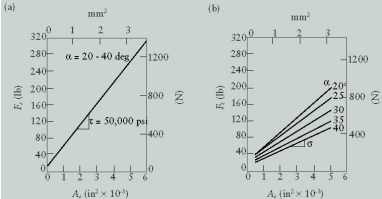
\includegraphics[width=\textwidth]{GraficiTaglioOrto}
\caption{Andamenti delle forze per il taglio ortogonale}
\label{fig:GarficiTaglioOrto}
\end{figure}

Nel grafico \ref{fig:GarficiTaglioOrto}.(a) è rappresentato l'andamento della forza di taglio 
$F_s$ giacente sul piano di taglio. Si osserva che tale forza aumenta all'aumentare dell'area 
del piano di taglio. 
Dunque è importante diminuire proprio quest'ultima: attraverso le strategie per 
aumentare $\phi$ viste in precedenza. Oltretutto tale andamento non è influenzato 
dall'angolo di spoglia superiore.
L'ipotesi che porta a tale costruzione sta nel fatto che il materiale è supposto non
incrudente. Infatti: raggiunto tale valore di sforzo tangenziale $\tau$ il materiale si 
rompe. Nel caso di materiale incrudente: si avrà una curva più che lineare, in quanto la 
deformazione porterà all'irrigidimento nella zona di taglio che necessiterà di maggiore
forza per avere la separazione del materiale.

Nel grafico \ref{fig:GarficiTaglioOrto}.(b) viene rappresentata la forza normale al piano di 
taglio $F_n$.
Questa dipende dall'angolo di spoglia superiore.
L'effetto di tale forza è stato già evidenziato: questa fornisce una specie di compressione 
idrostatica sul piano di taglio portando il materiale ad essere più duttile.
Ciò spesso si traduce in un truciolo continuo che però è problematico per la continuazione
della lavorazione: in quanto ingombrante e pericoloso.

\begin{figure}
\centering
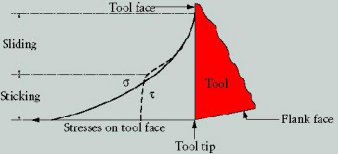
\includegraphics[width=\textwidth]{Sticking}
\caption{Tipologia di forze prementi sulla faccia dell'utensile}
\label{fig:sticking}
\end{figure}

Nel grafico \ref{fig:sticking} viene riportato il dettaglio sulla faccia superiore 
dell'utensile.
Si possono vedere due sezioni distinte:
\begin{description}
\item[\eng{Sliding}] in questa sezione si presenta lo scivolamento del truciolo sulla faccia
dell'utensile. Questo porta una cera forza resistente contro l'utensile di tipo $\tau$: ovvero 
di sforzo tangenziale. Si ha uno strisciamento completamente regolato dal coefficiente di 
attrito. Tale resistenza si annullerà nel momento in cui c'è distaccamento tra truciolo e 
faccia.
\item[\eng{Sticking}] nella zona di adesione si manifesta un particolare fenomeno per cui
il materiale del lavorato si accumula sulla punta dell'utensile. Ciò permette di generare una 
zona di ristagno che favorisce la separazione del materiale tra quello tagliato e il
truciolo. Di fatto in alcune occasioni può essere benefico per il tagliente in quanto
diventa uno strato protettivo. La resistenza portata da tale fenomeno diventa di pura 
deformazione $\sigma$. 
\end{description}

Al momento non si è ancora approfondita la finalità dell'angolo di spoglia inferiore $\theta$.
Idealmente servirebbe ad evitare lo strisciamento tra utensile e lavorato.
Siccome nella realtà bisogna considerare anche il ritorno elastico, non è possibile ottenere
un perfetto distaccamento tra utensile e lavorando. Dunque un po' di strisciamento si 
verifica in qualsiasi occasione. Ciò provoca usura dell'utensile.
Tra l'altro questo tipo di usura è la più severa per l'utensile.


\section{Taglio ortogonale realistico}
Il taglio del materiale non avviene più nel piano
di taglio, bensì sulla zona di taglio detta anche
\textbf{Zona di taglio primaria} mostrato in 
figura \ref{fig:TaglioOrtoRealScheme}.

\begin{figure}
\centering
\subfloat[][\emph{Schematizzazione del taglio ortogonale realistico}\label{fig:TaglioOrtoRealScheme}]
{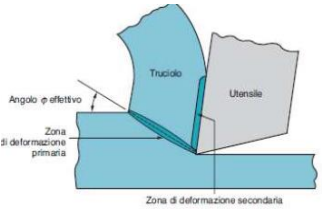
\includegraphics[width=0.5\textwidth]{TaglioOrtoRealScheme}}\\
\subfloat[][\emph{Tipologie di truciolo}\label{fig:Trucioli}]
{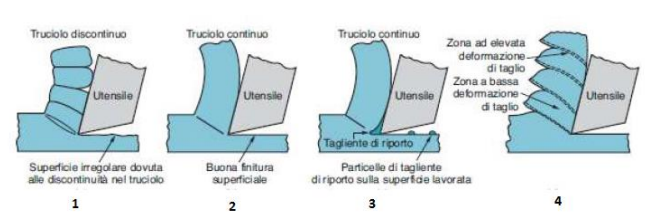
\includegraphics[width = \textwidth]{TaglioOrtoReal}}
\caption{Taglio ortogonale reale}
\label{fig:TaglioOrtoreal}
\end{figure}

Inoltre si osserva una zona deformata plasticamente, per cui si presenta un incremento della 
resistenza pari a quasi 3 volte la durezza nominale del pezzo lavorato.

Analizzando il comportamento del truciolo si possono
verificare delle situazioni, come illustrato in figura \ref{fig:Trucioli}:
\subsection{Truciolo continuo} Si verifica per velocità abbastanza basse. Come dice il nome Truciolo forma un continuo filamento di materiale.
Risulta più semplice lubrificare la faccia dell'utensile, abbassando $\beta$ come avevamo visto
in precedenza per diminuire la dimensione del piano di taglio. Dunque la zona di taglio resta più sottile
e la superficie uscirà dalla lavorazione con una 
finitura migliore.

Se da questa situazione si aumenta la velocità di
lavorazione, si va a formare una zona detta: 
\textbf{tagliente di riporto}.
Ciò è dovuto all'aumento della velocità con conseguente formazione della zona di ristagno
davanti alla faccia dell'utensile.
In particolare il tagliente di riporto:
\begin{itemize}
\item $\alpha$ aumenta per via per effetto della
zona di ristagno, per ciò si abbassa la forza di 
taglio.
\item In qualche misura protegge la faccia dell'utensile.
\item Può depositarsi sulla faccia del lavorato 
intaccandone la finitura superficiale.
\end{itemize}

Aumentando ulteriormente la velocità; la zona di taglio primario si assottiglia ulteriormente.
Comincia ad instaurarsi il fenomeno dello \eng{stiching}.
Il fenomeno si deve principalmente al riscaldamento
del materiale il quale crea adesione sulla faccia del
tagliente. Sarà, dunque, necessario aumentare la 
forza di taglio.

Si può già intuire che la velocità di taglio sarà 
strettamente legata alla temperatura generata durante la lavorazione.

Rimanendo nel tema del truciolo continuo si può verificare una situazione di truciolo continuo ma
ondulato

\subsubsection{Truciolo continuo ondulato}
È dovuto ad una variazione periodica nella forza di taglio. Possono esserci diversi motivi per cui 
si verifichi tale variazione: 
\begin{itemize}
\item Superficie rugosa, limita lo scorrimento del
tagliente.
\item Presenza di vibrazioni autoeccitate: se le vibrazioni sono dovute a forti variazioni nella superficie di taglio.
\item Distacchi del tagliente di riporto che va ad aderire alla superficie del materiale lavorato. 
Impone una maggiore forza perché l'utensile "deve"
far aderire tale riporto sulla superficie.
\item Vibrazioni forzate: generate dalla macchina 
e in genere dovute agli elementi elastici della macchina.
\item Quando si rompe il tagliente di riporto, portandosi via anche un pezzo del tagliente vero
e proprio.
\end{itemize}

Altra situazione particolare, di cui tenere nota, è la casistica in cui si forma il truciolo a dente di sega.

\subsubsection{Truciolo continuo a dente di sega}
Costituito da sezioni a diversa deformazione, la successione di zone spesse a bassa deformazione a zone fine di alta deformazione.
Le cause di tale comportamento è da imputarsi a:
\begin{itemize}
\item bassa conduttività termica del materiale,
per cui non riesce a smaltire il calore generato dalla lavorazione. 
\item Ciò spiega l'alternanza delle zone ad alta deformazione e bassa deformazione: le sezioni a bassa deformazione sono caratterizzate da un'alta temperatura relativa per cui l'utensile taglia
più facilmente il materiale. Una volta asportata una sezione di materiale, viene automaticamente smaltito
del calore "bloccato" nel materiale. Dunque la sezione successiva trova un calore minore, per cui il 
tagliente fa più fatica a tagliare e deforma di più 
il materiale. Per questo motivo le sezioni ad alta 
deformazione sono più fine.
\end{itemize}
Ultima casistica di truciolo, è quella del truciolo 
discontinuo.

\subsection{Truciolo discontinuo}
Si verifica in situazioni di velocità estremamente
basse su macchine scadenti a bassa rigidezza.
Altre situazioni per cui si va ad avere truciolo 
discontinuo sono:
\begin{itemize}
\item Per materiali che contengono inclusioni e fasi
secondarie che alzano le tensioni. Ciò provocano delle continue rotture di truciolo.
\item Situazioni di stick-slip.
\end{itemize}

Sebbene il truciolo continuo sia ricercato per favorire una finitura superficiale migliore, spesso
non è possibile tenere trucioli particolarmente lunghi. Durante la lavorazione un truciolo lungo
può essere d'intralcio all'operatore e alla macchina.

Allora si ha la necessità di rompere il truciolo.

\begin{wrapfloat}{figure}{O}{0pt}
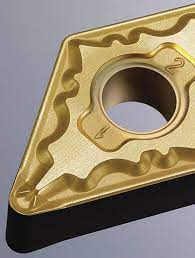
\includegraphics[width = 0.3\textwidth]{Rompitruciolo}
\caption{Esempi di rompi-truciolo}
\label{fig:Rompitruciolo}
\end{wrapfloat}


\subsection{La rottura del truciolo}
È particolarmente facile coi materiali fragili, più
complicato per quei materiali duttili che tendono
a formare dei trucioli continui.
Allora si ricorre a opportuni \textbf{rompi-truciolo},
inserti che possono essere fissati all'utensile o già
disegnati su esso, per favorire la rottura del 
truciolo ponendo ulteriore deformazione al materiale
asportato.
I rompi-truciolo hanno uno specifico valore efficace
di rottura del truciolo dipendente dalla profondità 
dello spessore indeformato: questa è una 
caratteristica della forma e dimensione geometrica 
del rompi-truciolo. In figura \ref{fig:Rompitruciolo} 
un dettaglio.

\section{Taglio obliquo}
Viene sfruttato maggiormente dalle aziende.
Garantisce una lavorazione che necessita di maggiore
forza per il taglio, ma la vita del utensile
è più lunga.

A differenza del taglio ortogonale dove si veniva
a formare un truciolo continuo a forma di spirale.
Nel taglio obliquo si forma un truciolo a forma 
elicoidale, che ha una propria tendenza geometrica
a spostarsi via dal punto di lavorazione.
Si evita la necessità di rompere il truciolo, anche 
se è una pratica che comunque viene mantenuta.
È opportuno definire un nuovo angolo di spoglia 
superiore.
\begin{align}
\alpha_e &:= \text{Angolo di spoglia efficace}\\
\alpha_n &:= \text{Angolo di spoglia normale}\\
&\text{In generale: }\alpha_e > \alpha_n
\end{align}
Vale che più il tagliente è inclinato, più aumenta $\alpha_e$ 
e di conseguenza $F_c$ diminuisce.

Nel caso in cui il tagliente non sia più grande del
pezzo in lavorazione, lo spessore del truciolo 
indeformato non è più sufficiente a descrivere i 
fenomeni legati a questo. Dunque è necessario parlare
di \textbf{avanzamento} $f$. Inoltre si introduce 
la \textbf{profondità di passaggio} $w$.

\begin{figure}
\centering
\subfloat[][\emph{Schema del taglio obliquo}\label{fig:TaglioObliquoScheme}]
{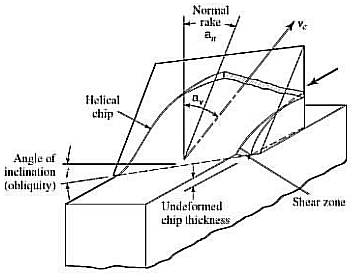
\includegraphics[width = \textwidth]{TaglioObliquo}}\\
\subfloat[]
[\emph{Parametri del taglio ortogonale per confronto}\label{fig:TaglioObliquoParam1}]
{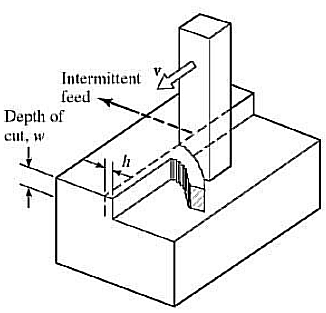
\includegraphics[width = 0.4\textwidth]{TaglioObliquoParam1}}\quad
\subfloat[][\emph{Ulteriori parametri del taglio obliquo}\label{fig:TaglioObliquoParam2}]
{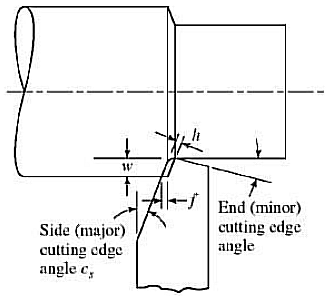
\includegraphics[width = 0.4\textwidth]{TaglioObliquoParam2}}
\caption{Il taglio obliquo}
\label{fig:TaglioObliquo}
\end{figure}

\subsection{Tornitura}
Un esempio di tornitura è riportato alla figura \ref{fig:TaglioObliquoParam2}.
\begin{wrapfloat}{figure}{O}{0pt}
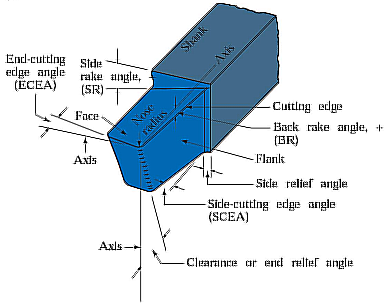
\includegraphics[width = 0.5\textwidth]{Utensile}
\caption{Esempio di utensile per tornitura}
\label{fig:UtensileTornitua}
\end{wrapfloat}

\begin{itemize}
\item utensile con tagliente inclinato
\item $f$ è ortogonale al tagliente e rappresenta 
l'avanzamento;
\item $w$ è la profondità di passata
\item $h$ è lo spessore di truciolo indeformato.
\end{itemize}

Con l'utensile inclinato si ha una maggiore forza 
necessaria al taglio, però si aumenta 
considerevolmente la durata dell'utensile.
Indubbiamente la caratterizzazione del tagliente 
risulta più complicata. Si ha l'ulteriore vantaggio
di avere un utensile che può presentare più 
taglienti.

\subsection{Calcolo della forza ed energia}
Siccome per via del tipo di lavorazione non siamo in grado di sfruttare
la deformazione per flusso plastico a causa della velocità decisamente 
superiore.
È decisamente importante sapere quanta energia o potenza è necessaria 
per effettuare la lavorazione. Perché tale potenza sarà quella che il
motore della macchina deve fornire all'utensile.

A differenza della lavorazione per deformazione plastica in cui 
la "pressa" deve fornire una certa pressione per permettere la 
deformazione. Nell'asportazione si possono cambiare alcuni
parametri in base anche punto della lavorazione si è.
Continuando a lavorare il pezzo.

Resta evidente come la parametrizzazione della lavorazione sia
definitivamente importante: in modo da garantire la continuazione
della lavorazione, cambiando alcune condizioni senza interromperla.
Anche per il fatto che fermando la lavorazione peggiora la finitura.

Nella definizione dell'energia necessaria si sa che si va a commettere
un'errore di circa il $20\%$.
Di fatto sarebbe necessario conoscere $\beta$, ma non è facile da valutare.
Allora si può valutare la \textbf{pressione di taglio}.

\begin{equation}
p_c = \frac{\overbrace{F_c}^{\text{Componente parallela alla velocità di taglio}}}{h \cdot w}
\end{equation} 
Per ottenere una forma di energia basta integrare la pressione
o forza per la lunghezza del lavoro eseguito ovvero:
\begin{equation}
l := \text{lunghezza di taglio}\\
\end{equation}

\begin{definition}{Pressione ed energia di taglio specifica}{PEspec}
\begin{subequations}
\begin{align}
p_c &= \frac{F_c}{h \cdot w} \\
E_1 &= p_c \cdot \frac{l}{l} \:[\unit{\W\s/\m^3}]
\end{align}
\end{subequations}
Dove $p_c$ è la pressione specifica di taglio e $E_1$ è l'energia specifica.
\end{definition}

\begin{definition}{Fattore di rimozione}{FattRim}
Si può definire anche il Fattore di rimozione del materiale:
\begin{equation}
k_1 = \frac{1}{E_1}
\end{equation}
dove $k_1$ rappresenta la quantità di materiale asportato da una macchina
a motore a potenza unitaria.
\end{definition}

I 3 parametri non sono costanti per un materiale perché dipendono anche dai
parametri di processo quali spessore di truciolo indeformato, angolo di spoglia e
velocità di taglio.
L'energia spesa nella zona di taglio primaria e la quantità di materiale rimosso
sono proporzionali allo spessore di truciolo indeformato.
\begin{equation}
E = k \cdot h \cdot p \cdot l
\end{equation}

Nella zona di taglio primaria la pressione specifica, l'energia specifica e il fattore di
rimozione del materiale sono costanti del materiale.
L'energia consumata sul dorso dell'utensile è indipendente dallo spessore di
truciolo indeformato, possiamo ritenerla quasi costante.
Quindi vale:
\begin{equation}
\frac{E_d}{h \cdot p \cdot l} \neq cost.
\end{equation}

A questo punto si è definita una relazione in cui si può già definire la forza necessaria.
C'è da tenere in considerazione l'usura dell'utensile: in quanto quest'ultima tende
a richiedere una maggiore pressione da parte del tagliente per tagliare.
Siccome l'usura del tagliente è un argomento che richiede la considerazione di diversi
parametri e che tali non possono sempre essere determinatiti così facilmente.
Semplicemente si aggiunge un $30\%$ in più all'energia necessaria.

Ulteriori parametri derivati dai precedenti sono:
\begin{definition}{Ulteriori Parametri}{UltParam}
Sono delle derivazioni dei parametri visti precedentemente.
\begin{equation}
E = E_1 \left(\frac{h}{h_{ref}}\right)^{-a} = E_1 \cdot h^{-a}
\end{equation}
Dove $E$ è l'energia di lavorazione, $h_{ref} = 1\unit{\mm}$ è lo spessore indeformato di 
riferimento e $a \approx 0.3$.
Da cui si può definire la potenza necessaria per la lavorazione:
\begin{equation}
Power(W) = \frac{E \cdot V_t}{\eta}
\end{equation}
Dove $V_t$ è la velocità di taglio, $\eta$ il rendimento della macchina.
Da cui si può ottenere la forza necessaria per il taglio:
\begin{equation}
F_c = \frac{Power(W)}{v}
\end{equation}
\end{definition}

\subsection{Temperature}
Siccome la lavorazione prevede di "muovere" del materiale dentro se stesso
questo provoca un accumulo di energia danti alla faccia dell'utensile.
Tale energia rimane nella maggior parte nel truciolo.

\begin{wrapfloat}{figure}{I}{0pt}
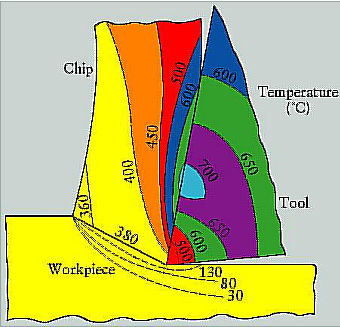
\includegraphics[width = 0.4\textwidth]{Temperature}
\caption{Analisi termica dell'asportazione di truciolo}
\label{fig:Temp}
\end{wrapfloat}

Come si vede dalla figura \ref{fig:Temp}, le temperature raggiunte non sono da 
trascurare: si può arrivare a $\approx 1000\unit{\celsius}$ sulla faccia dell'utensile.
Sappiamo che con l'aumento della temperatura, aumentano il numero di dislocazioni
interne al materiale che diventa più duttile dunque più facile da lavorare.

La maggior parte dell'energia resta interna al truciolo che, portando con se del
calore, abbassa la temperatura del lavorato. Resta il calore trasferito 
all'utensile, il quale tende ad aumentare la temperatura considerevolmente.
Infatti, come si vede proprio dalla figura \ref{fig:Temp}, è proprio
l'utensile a mostrare le temperature più alte. Ciò impone che il
materiale dell'utensile debba essere di un materiale alto resistente a caldo.

\begin{figure}
\centering
\subfloat[][\emph{Schema delle isoterme sulla faccia dell'utensile}\label{fig:TempUtensile}]
{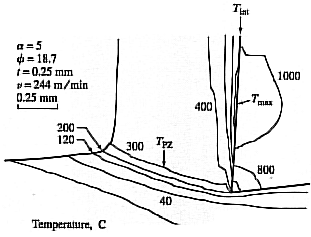
\includegraphics[width = 0.4\textwidth]{TempScheme}}\quad
\subfloat[][\emph{Relazione tra velocità di lavorazione e temperatura}
\label{fig:TempVel}]
{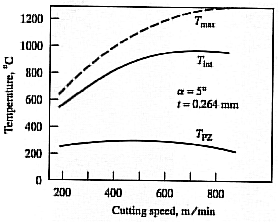
\includegraphics[width = 0.4\textwidth]{TempVel}}
\caption{Temperature durante le lavorazioni ad asportazione}
\label{fig:TempLav}
\end{figure}

Come fatto in precedenza, si è cercato di relazionare la temperatura con la
velocità di lavorazione: legame che fisicamente è noto ma non così facile 
da porre analiticamente.

\begin{equation}
T_t = E \left( \frac{v \cdot h}{k \cdot \rho \cdot c}\right)^{1/2}
\end{equation}
Dove:\\
\begin{tabularx}{\textwidth}{cX}
$E_1$ & Energia specifica\\
$v$ & Velocità di taglio\\
$h$ & Spessore di truciolo indeformato\\
$k$ & Conduttività termica\\
$\rho$ & Densità\\
$c$ & Calore specifico 
\end{tabularx}\\
Se ne ottiene una stima della temperatura media sulla faccia dell'utensile.
Come spesso succede nei sistemi fisici reali, tutta l'energia donata dalla
macchina al materiale viene trasformata in calore.
Indubbiamente durante le lavorazioni non si deve superare la temperatura di fusione
del materiale lavorato: altrimenti si va ad ottenere una lavorazione molto grossolana di
cui non si riesce a controllarne i parametri.
I materiali a bassa fusione risultano più facili da lavorare.
Inoltre, per lavorazioni di finitura particolarmente restrittive, bisogna considerare
le variazioni dimensionali dovute alla dilatazione termica.

\subsection{Fluidi da taglio}
In industria ed artigianato, queste lavorazioni vengono spesso
effettuate con l'assistenza dei fluidi da taglio.
Questi hanno diverse funzioni per la lavorazione, tipo:

\begin{description}
\item[Lubrificazione] si cerca di abbassare l'attrito nella
lavorazione, per favorire un'asportazione più agile.
Il problema sta nel portare il fluido nella zona di lavorazione,
impedito del movimento del truciolo.
Perciò aumentando la velocità di lavorazione di ha una 
lubrificazione meno efficacie.
\item[Raffreddamento] Diminuendo la temperatura sulla faccia 
dell'utensile si può lavorare a velocità più alte.
Al contempo questo rappresenta un problema: se l'utensile non è 
costantemente immerso nel materiale, il raffreddamento potrebbe
diventare uno shock termico per via delle forti variazioni di 
temperature.
\item[Rimozione del truciolo] Utilizzando dei sistemi ad alta
pressione si possono sfruttare gli utilizzi precedenti mentre 
si spostano i trucioli dalla zona i lavorazione.
\end{description}

%%%%%%%%%%%%%%%%%%%%%%%%%%%%%%%%%%%%%%%%%%%%%%%%%%%%%%%%%%%%%%%%%%%
% Capitoli già realizzati									    	%
%%%%%%%%%%%%%%%%%%%%%%%%%%%%%%%%%%%%%%%%%%%%%%%%%%%%%%%%%%%%%%%%%%%
\newpage
\chapter{Lavorazioni al trapano}\label{chp:LavTrapano}
È una macchina utensile molto diffusa.
In realtà realizza una sola lavorazione: crea dei fori.
Data la necessità di creare dei fori, se ne capisce la fondamentalità.

\begin{figure}
\centering
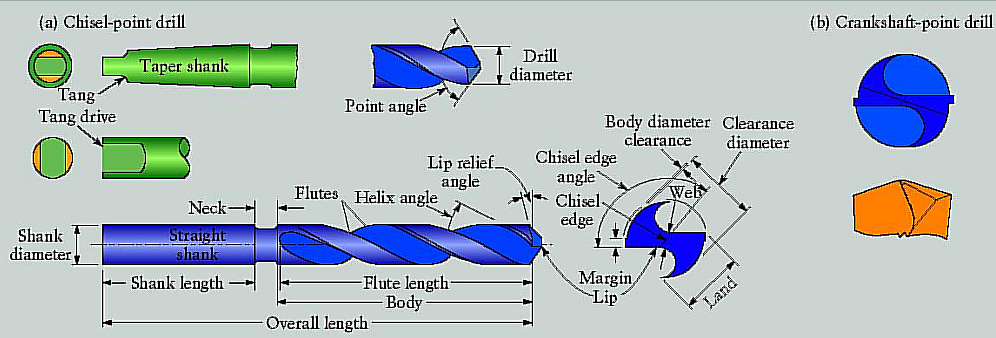
\includegraphics[width = \textwidth]{Trapanatura}
\caption{Alcune punte da trapano per diverse forature}
\label{fig:Tapanatura}
\end{figure}

dalla figura \ref{fig:PunteTrapano} si può vedere che esistono diverse punte da trapano.
Si può già fare un confronto tra le punte da trapano e gli utensili
monotagliente visti per il tornio.
In genere l'utensile monotagliente tende a flettere parecchio, mentre nelle punte da trapano 
le forze sono bilanciate per via della forma del tagliente.
In più le punte presentano delle scanalature elicoidali che dovrebbero assolvere
a due funzioni:
\begin{itemize}
\item rimuovere il truciolo dalla zona di taglio
\item favorire la lubbrificazione del tagliente
\end{itemize}
In realtà non fanno correttamente nessuna delle due operazioni.

\begin{figure}
\centering
\subfloat[][\emph{Principali punte da trapano}
\label{fig:PunteTrapano}]
{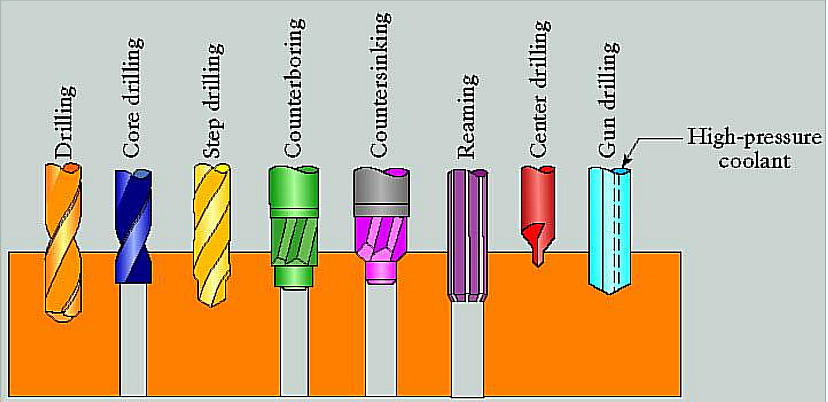
\includegraphics[width = \textwidth]{PunteTrapano}}\\
\subfloat[][\emph{Punte per foratura}\label{fig:PunteForatura}]
{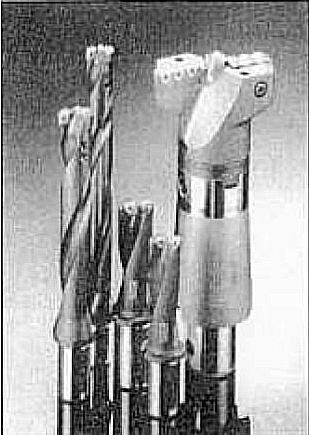
\includegraphics[width = 0.4\textwidth]{PunteForatura}}\quad
\subfloat[][\emph{Esempi di mecchie}\label{fig:UlterioriPunte}]
{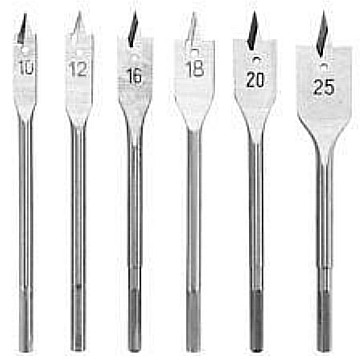
\includegraphics[width = 0.4\textwidth]{UlterioriPunte}}
\caption{Varie tipologie di punte da trapano}
\label{fig:Punte}
\end{figure}

Nella foratura le forze sono bilanciate. Più importante è da considerare:
Man mano che ci si avvicina all'asse della punta i taglienti lavorano ad una velocità di taglio
moinore, per cui la finitura superficiale peggiora.
È per questo motivo che i talgienti delle punte da trapano non arrivano al centro della punta.
Dunque la punta è realizzata con forma conica in modo tale da spostare il materiale in lavorazione 
verso le zone di lavorazione laterali. Insomma funge da scalpello allontanando il materiale
dall'asse di rotazione. Saranno dopo i taglienti ad asportarlo effettivamente. 
Tra l'altro, la forza per spostare il materiale è la maggiore parte di forza utilizzata per tale lavorazione.
Infatti di solito si utilizza prima una foratura più fina per una prima asportazione, poi viene 
eseguita la foratura principale che porta il foro alla dimensione desiderata.

Ovviamente lo scalpello della punta si usura e dunque si dovrà applicare maggiore forza alla punta.
Per cui la forma dello scalpello si è evoluta in modo da rendere minore la forza di spinta da applicare alla 
punta. In più, sulle scanalature elicoidali sono presenti delle scanalature ulteriori che fungono da 
rompitruciolo.

Ulteriore problematica è quella dello spostamento dell'asse della punta. Allora si utilizza una punta
da centri per "indicare" alla punta da trapano la direzione di foratura.

L'angolo dell'elica rappresenta l'angolo di spoglia periferica della punta.
L'angolo di spoglia diminuisce avvicinandosi al centro della punta.
Per favorire lo spostamento del truciolo, spesso si utlizzano delle punte con angolo d'elica particolarmente 
elevato.

Dove c'è dello spazio grigio indica il fatto che si deve eseguire un prima foratura prima di usare 
quell'utensile.

Con riferimento alla figura \ref{fig:PunteTrapano}, rispettivamente sono:
\begin{enumerate}
\item Punta da trapano classica;
\item Va usato dopo l'utensile precedente e semplicemente allarga il foro
\item Realizza un foro a due diametri detta anche \emph{step-drilling}
\item Realizza un gradino su un foro già realizzato, viene detta anche \emph{lamatura}
\item Stesso obbiettivo della precedente \emph{Utensile a lamare}
\item stesso del precedemnte \emph{Utensile a svasare}
\item Utensile di \emph{alesatura} va semplicemente a rifinire il foro fatto in precedenza.
\item Punta da centri, realizza un piccolo for perguidare la punta da trapano.
\item È un utensile utilizzato in particolare per lavorazioni su lamiere.
\end{enumerate}

In genereale le punte da trapano sono degli utensili di materiali monoblocclo. Esistono anche delle punte
da trapano che presentano degli inserti. Certo si hanno dei fori un po' magiori per via delle dimensioni
degli inserti.
Eventualmente si ricorre a dei trattamenti termochimici per aumentare la durata della punta.

Ulteriori utensili sono mostrati in figura \ref{fig:UlterioriPunte}.
Le Mecchie sono utilizzate per realizzare fori di piccola profondità.
Le mecchie di forma conica permettono di realizzare dei fori in base alla profondità a cui si spinge la punta
a diametro variabile. Spesso usate per lavorazioni su lamiere.

\begin{figure}
\centering
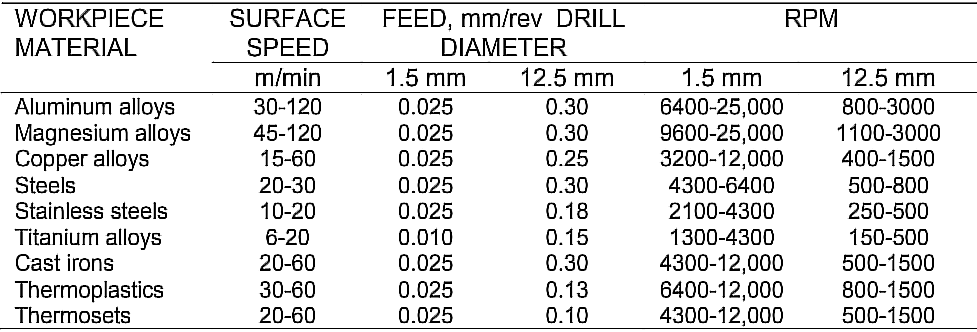
\includegraphics[width = \textwidth]{VelTrapanatura}
\caption{Velocità consigliate di trapanatura}
\label{fig:Veltrapanatura}
\end{figure}

\section{Tipologie di trapani}

\begin{figure}
\centering
\subfloat[][\emph{Esempio di trapano semplice}\label{fig:Trapano}]
{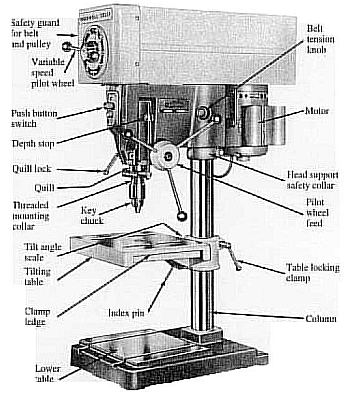
\includegraphics[width = 0.4\textwidth]{Trapano}}\quad
\subfloat[][\emph{Esempio di trapano a controllo numerico}\label{fig:TrapanoCNC}]
{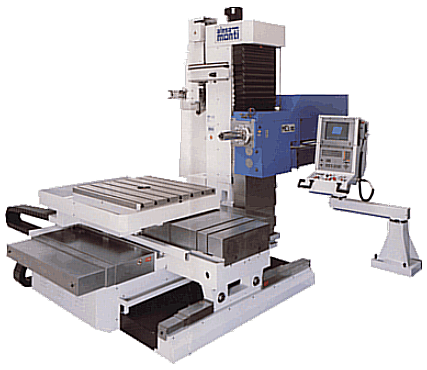
\includegraphics[width = 0.4\textwidth]{TrapanoCNC}}\\
\subfloat[][\emph{Particolare sulle punte alesatrici}\label{fig:PuntaFresatrice}]
{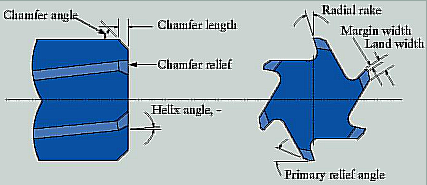
\includegraphics[width = 0.5\textwidth]{PuntaFresatrice}}
\caption{Alcuni esempi di trapani e dettaglio punta alesatrice}
\label{fig:Trapani}
\end{figure}
Alcuni esempi di trapanio sono riportati alle figure \ref{fig:Trapani}. Risulta molto riduttivo parlare di macchine che eseguono solo trapanature (nonostante esistano e vengano tutt'oggi prodotte) perché ormai soppiantate dai centri di lavoro \ac{FMS}.
Di fatto l'evoluzione dei centri \ac{FMS} ha ormai inglobato quasi tutte le possibili lavorazioni per asportazioni di truciolo in un'unica macchina.
Di questo se ne parlerà nel capitolo \ref{chp:MacchineUtensili} a pagina \pageref{chp:MacchineUtensili}.

Piccolo approfondimento per le punte da alesaggio.\\
Le punte da alesaggio \ref{fig:PuntaFresatrice} hanno scanalature piccole, questo perché si ha meno materiale da rimuovere, in più si ha una maggiore rigidezza dell'utensile per via del maggiore spessore del centro.
In generale gli utensili alesatori hanno angoli di elica sono molto molto piccole o addirittura cilindriche.

\chapter{Fresatura}\label{chp:Fresatura}
È la lavorazione più versatile che si può trovare in officina, permette di realizzare la più grande varietà di forme.
Un esempio è quello della fresatrice orizzontale: \ref{fig:FresaOrizzontale} determinato dall'asse di rotazione dell'utensile.
\begin{wrapfloat}{figure}{O}{0pt}
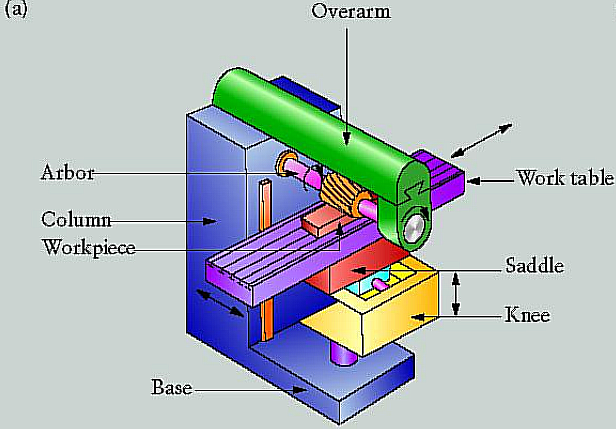
\includegraphics[width = 0.4\textwidth]{FresaOrizzontale}
\caption{Esempio di fresatrice orizzontale}
\label{fig:FresaOrizzontale}
\end{wrapfloat}
L'utensile può presentare taglienti elicoidali sia cilindrici.

Siccome la varietà di lavorazioni è alta, anche la gamma di utensili è piuttosto ampia.

L'evoluzione della lavorazione ha portato al fatto che gli utensili non sono sostenuti da due "cerniere".
Piuttosto si utilizzano utensili fissati a singolo punto.
Il tipo ideale di fresatura si chiama \emph{fresatura periferica}.

\section{Fresatura periferica}
Come anticipato, l'utensile può essere ad elica o a scanalature cilindriche. In genere si preferisce il tagliente ad elica perché subisce meno urti e si possono avere più taglienti immersi sul materiale contemporaneamente.
 
Le eliche possono essere in concordanza \ref{fig:FresaConc} o opposizione \ref{fig:FresaOpp}.
La differenza, oltre che alle direzioni di lavorazione e alimentazione sta anche nel metodo di asportazione. 
Infatti nella lavorazione in concordanza il tagliente, in figura \ref{fig:TaglConc}, incontra immediatamente la superficie del lavorato. Ciò provoca urti più alti al tagliente e in potrebbe incontrare pure degli ossidi che rendono il materiale più duro.

Mentre la lavorazione in opposizione, figura \ref{fig:TaglOpp}, presenta un problema di deformazione elastica: siccome lo spessore indeformato è nullo, il tagliente andrà a schiacciare il materiale andandolo a subire il successivo comportamento elastico.

\begin{figure}
\centering
\subfloat[][\emph{Fresatura in opposizione}\label{fig:FresaOpp}]
{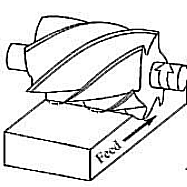
\includegraphics[width =0.4\textwidth]{FresaOpp}}\quad
\subfloat[][\emph{Fresatura in concordanza}\label{fig:FresaConc}]
{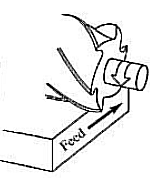
\includegraphics[width = 0.4\textwidth]{FresaConc}}\\
\subfloat[][\emph{Dettaglio del tagliente in opposizione}\label{fig:TaglOpp}]
{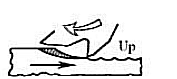
\includegraphics[width = 0.4\textwidth]{TaglOpp}}\quad
\subfloat[][\emph{Dettaglio del tagliente concorde}\label{fig:TaglConc}]
{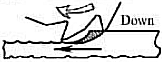
\includegraphics[width = 0.4\textwidth]{TaglConc}}
\caption{Fresatura in opposizione e concordanza}\label{fig:DirFresa}
\end{figure}

In generale si sfrutta la fresatura in concordanza nel caso in cui si predilige una migliore finitura superficiale e il materiale non è stato trattato a caldo: per cui non presenta ossidi superficiali che potrebbero consumare molto rapidamente i taglienti.
Altrimenti si sfrutta la fresatura in opposizione al netto delle peggiori tolleranze dimensionali ottenibili per via del ritorno elastico e la maggiore rigidezza della macchina necessaria per via dello scambio di forze che si va a verificare durante la lavorazione.

La lavorazione in definitiva viene detta anche \emph{spianatura}. 
A differenza di quanti visto per la piallatrice o levigatrice, la lavorazione risulta più veloce in quanto non è necessaria la corsa di ritorno e l'utensile può essere parecchio largo.

La spianatura può essere realizzata anche tramite utensile a sbalzo monotagliente.

\section{Fresatura verticale}
In questo caso si ha l'asse dell'utensile in verticale rispetto al lavorato. 
Attenzione che l'utensile è a sbalzo e non più fissato a due punti, quindi generalmente più rigido.
Può essere che queste macchine sfruttino una tecnologia ibrida per cui possono realizzare sia lavorazioni
in verticale che in orizzontale.
\begin{wrapfloat}{figure}{I}{0pt}
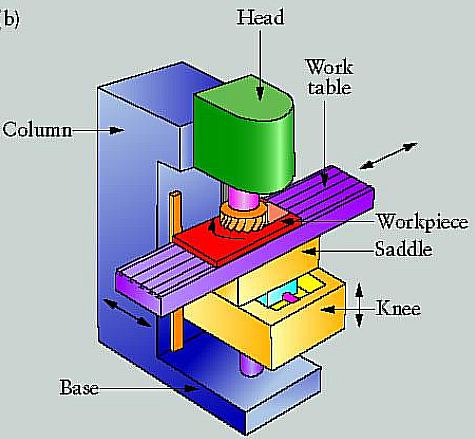
\includegraphics[width = 0.4\textwidth]{FresaVert}
\caption{Esempio di fresa verticale}
\label{fig:FresaVert}
\end{wrapfloat}

\begin{quote}
\emph{Come mai si preferisce un'utensile a sbalzo rispetto ad uno più rigido magari fissato in due punti?}
\end{quote}

È più facile cambiare utensile e può essere fatto automaticamente. Anche l'accessibilità alla zona di lavoro
non è da sottovalutare.
L'affermazione di tali macchinari è, dunque, puramente pratico.
Per cui si preferisce che l'utensile sia a sbalzo.

\subsection{Fresa a codolo}
La fresa a codolo, in figura \ref{fig:FresaCodolo}, è molto simile ad un trapano, ma la punta non presenta lo scalpello in virtù del fatto che l'elica non ha lo scopo di effettuare una foratura. Bensì l'elica ha lo scopo di evitare degli urti del tagliente che teoricamente potrebbe essere perfettamente cilindrico.
La tipica lavorazione di questa macchina è l'ottenimento di oggetti a piani paralleli.
Si ottengono dei gradini per via della lavorazione a piani paralleli, quindi sarà necessaria una successiva passata di finitura per ottenere una forma continua.
Tra l'altro, i piani non per forza devono essere orizzontali, possono essere anche verticali o a diversa inclinazione.
Indubbiamente l'automazione di queste macchine è fondamentale. Le quali possono realizzare delle forme che non sarebbero ottenibili con altre macchina.
In generale macchine ad alta automazione vengono anche chiamate \emph{centro di lavoro}.
Sono delle macchine ad alta automazione che uniscono i vantaggi delle principali lavorazioni per asportazione di truciolo.
Realizzano lavorazioni su tutte e 5 le facce del pezzo (La faccia di riferimento è quella appoggiata al porta-pezzo). In inglese \ac{FMS}.

Una prodotto tipico di queste lavorazioni sono gli stampi.

\begin{wrapfloat}{figure}{O}{0pt}
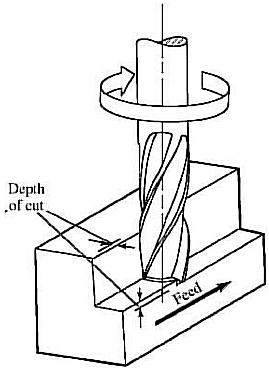
\includegraphics[width = 0.3\textwidth]{FresaCodolo}
\caption{Schematizzazione della fresatura a codolo}
\label{fig:FresaCodolo}
\end{wrapfloat}

Per ridurre tale condizione, evitando di fare più passate successive, si possono usare delle frese a codolo a testa sferica, \ref{fig:FresaSferica}, che evitano il problema della velocità radiale nulla al centro della punta. Vanno usate ad un'inclinazione di circa $15\unit{\degree} \div 30\unit{\degree}$ per mantenere una buona velocità radiale in qualsiasi punto dei taglienti. 

\begin{figure}
\centering
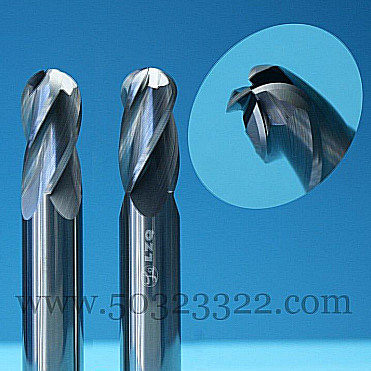
\includegraphics[width = 0.4\textwidth]{FresaSferica}
\caption{Esempio di frese a testa sferica}
\label{fig:FresaSferica}
\end{figure}

\section*{Il controllo numerico}
\begin{description}
\item[Asse controllato] quando di quell'asse se ne può controllare posizione e velocità
\end{description}

\begin{quote}
Quanti assi controllati per ogni tipo di lavorazione?
\end{quote}

Per il trapano ad esempio è sufficiente un solo asse, l'avanzamento della punta.
Per il tornio ne bastano due: uno in direzione ortogonale all'asse di rotazione del pezzo e uno in direzione 
parallela.
Per la fresatrice invece sono 3.

Negli assi mandrino, si controllano solamente la velocità quindi non viene considerato come asse controllato.

Quando si parla di macchine a più assi (4,5) si possono avere delle rotazioni dell'utensile.
Eventualmente Si possono sfruttare degli utensili a testa sferica (opportunamente inclinati per non avere 
velocità nulle sull'asse di rotazione).

\chapter{Altre Lavorazioni}\label{chp:AltreLav}
\section{Taglio con sega}
Risulta una forma di fresatura, con dei taglienti molto fini.
In genere si sfrutta un'utensile cilindrico molto fino al quale vengono
attaccati i taglienti che possono essere di materiale diverso da quello 
dell'utensile stesso.
Viene spesso utilizzata per separare due parti di materiale.
In figura \ref{fig:Seghe} ne sono presentate alcune.

\begin{figure}
\centering
\subfloat[][\emph{Tipologie principali di seghe utilizzate in industria}
\label{fig:Seghe}]
{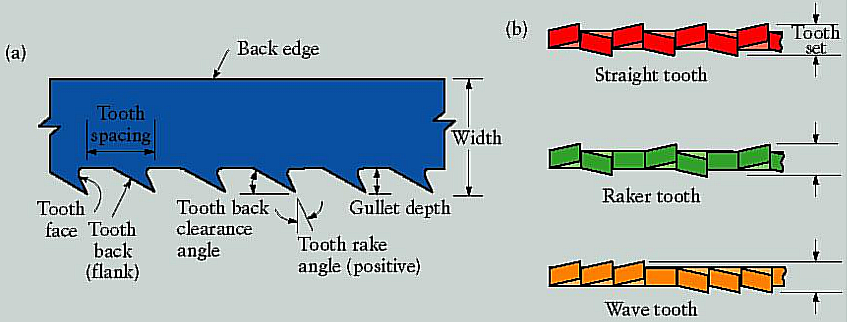
\includegraphics[width = \textwidth]{Seghe}}\\
\subfloat[][\emph{Esempio di inserto per sega}\label{fig:SegheInserti}]
{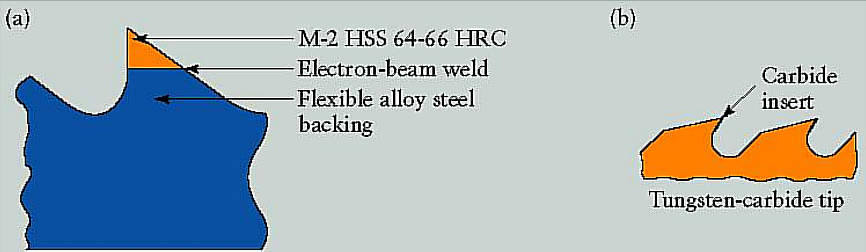
\includegraphics[width = \textwidth]{SegheInserti}}
\caption{Breve descrizione delle seghe industriali}
\label{fig:SegheInd}
\end{figure}

\section{Brocciatura e taglio di filetti}
\subsection{La brocciatura}
si ha sempre un'utensile di forma, di cui se ne controlla solo il moto primario. Ciò è possibile perché l'avanzamento viene realizzato per cui
sarà il tagliente ad avanzare autonomamente.
La maggior parte del materiale verrà asportata di taglienti detti di sgrossatura per poi essere finiti dai taglienti di finitura.
Ad ogni componente da realizzare il suo utensile.

Solitamente si eseguono dei fori non circolari. Si effettua da prima 
un foro circolare per poi passare con la \textit{broccia}, in figura \ref{fig:Broccia}, che realizza forme particolare come richiesto.

\begin{figure}
\centering
\subfloat[][\emph{Esempio e parametrizzazione di una broccia}\label{fig:Broccia}]
{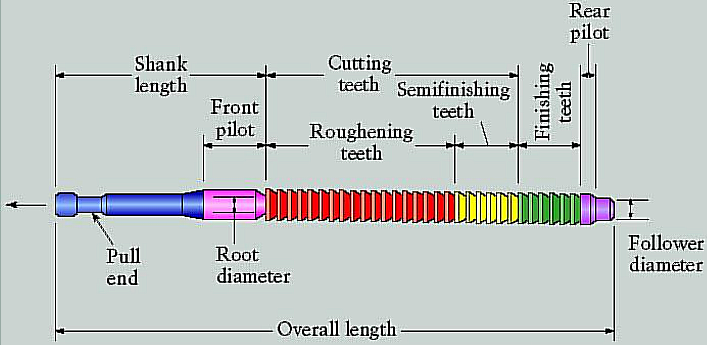
\includegraphics[width = \textwidth]{Broccia}}\\
\subfloat[][\emph{Dettaglio della lavorazione tramite broccia}
\label{fig:DettaglioBroccia}]
{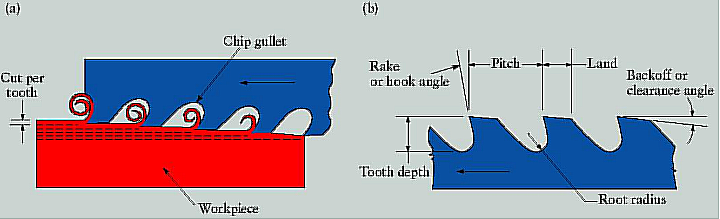
\includegraphics[width = \textwidth]{DettaglioBroccia}}
\caption{Brocciatura}
\label{fig:Brocciatura}
\end{figure}

Si tratta di un utensile parecchio costoso per via del fatto che è un'utensile massiccio. Viene utilizzato solitamente per la produzione in grande serie, per ammortizzare meglio il costo.
I taglienti asportano il materiale in maniera progressiva, in figura \ref{fig:DettaglioBroccia}, a differenza di quanto visto per altri utensili precedenti.
Da considerare l'eventuale deflessione dell'utensile posta dalla resistenza
meccanica del materiale lavorato, soprattutto per brocciature esterne.
Per quelle interne non sussiste il problema.
La boccia può essere spinta nel materiale oppure tirato.
Se spinto si sfruttano delle brocce piuttosto corte per via dell'ampia
deflessione che si va a generare.
Discorso diverso nel caso in cui l'utensile viene tirato, per cui si possono avere brocce fino a $2\unit{\m}$.

\subsection{Filettature}
L'operazione non è molto diversa da quella precedente: cambia il tipo di moto applicato all'utensile: nella filettatura si ha un moto di rotazione
elicoidale per cui l'utensile avanza radialmente e longitudinalmente.

\begin{figure}
\centering
\subfloat[][\emph{Utensile per filettatura interna}\label{fig:FilettaturaEsterna}]
{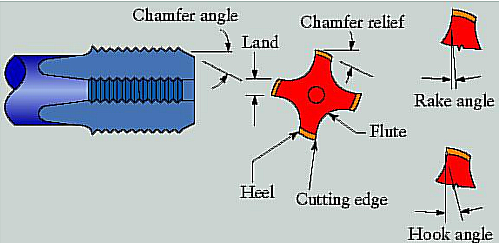
\includegraphics[width = 0.4\textwidth]{FilettaturaInterna}}\quad
\subfloat[][\emph{Utensile per filettatura esterna}]
{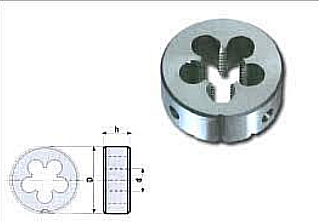
\includegraphics[width = 0.4\textwidth]{FilettaturaEsterna}}
\caption{Utensili per filettature}
\label{fig:Filettature}
\end{figure}

Normalmente la filettatura viene realizzata tramite deformazione plastica,
si ha incrudimento per lavorazione a freddo, non si asporta materiale e dunque le fibre del materiale non vengono tagliate orientandole in senso
assiale rispetto alla filettatura dando ulteriore resistenza meccanica.

\section{Aspetti conclusivi}
Alla figura \ref{fig:TolleranzeFiletti}, vengono riportate quali sono le principali lavorazioni ottenibili per asportazione di truciolo. Vengono anche specificate le tolleranze minime ottenibili.
Mentre alla figura \ref{fig:ProductionRates}, sono indicati quali siano le produttività.
\begin{figure}
\centering
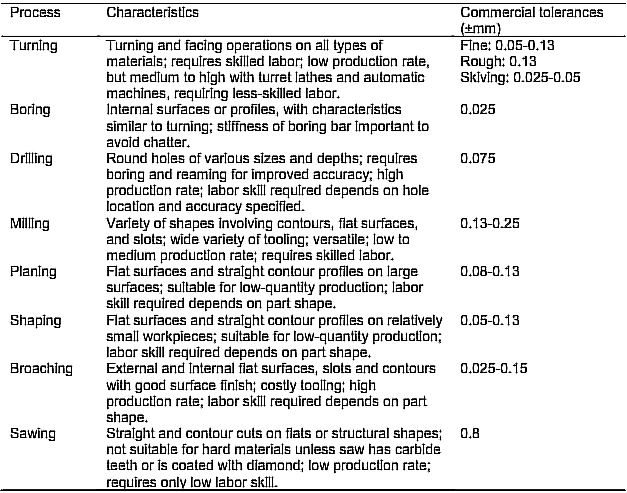
\includegraphics[width = \textwidth]{TolleranzeFiletti}
\caption{Riepilogo lavorazioni per asportazione di truciolo}
\label{fig:TolleranzeFiletti}
\end{figure}
\begin{figure}
\centering
\includegraphics[width = \textwidth]{ProductionRates}
\caption{Indicazioni sulla produttività delle specifiche lavorazioni per asportazione di truciolo}
\label{fig:ProductionRates}
\end{figure}

\section{Produzione di ingranaggi}\label{sc:Ingranaggi}
Per la produzione di ingranaggi si sfruttano quasi tutte le lavorazioni che si sono viste in precedenza come evidenziato dalla figura \ref{fig:Ingranaggi}.
In particolare, gli ingranaggi per applicazioni critiche, sono ancora realizzati tramite lavorazioni per asportazione di truciolo. Ciò garantisce un'ottima finitura di forma, arrivando a tolleranze molto restrittive.
Spesso sono lavorazioni di forma, con moto alternativo (caso della lamatura), oppure rotativo (caso della fresatura).

\begin{figure}
\centering
\includegraphics[width = \textwidth]{Ingranaggi}
\caption{Alcuni utensili per la produzione di ingranaggi}
\label{fig:Ingranaggi}
\end{figure}

Più complicata è la realizzazione di ingranaggi conici.
Si devono utilizzare degli utensili di forma, su macchine più adatte per 
tale scopo.  %Asportazione di truciolo
\cleardoublepage \chapter{Variabili di processo per lavorazioni in asportazione di truciolo}
\label{chp:VarProcAsportazione}
GLi aspetti principali da considerare per tali lavorazioni sono:
\begin{itemize}
\item Finitura superficiale
\item lavorabilità,
\item forma, 
\item dimensioni, 
\item tolleranze,
\item tipo di lavorazione, 
\item macchine disponibili, 
\item valutazioni economiche
\end{itemize}

La prima decisione necessaria è la sequenza delle operazioni da eseguire.
Per ogni lavorazione bisogna scegliere velocità di taglio e avanzamento in funzione dei materiali del pezzo e utensile. Anche la fase della lavorazione 
va tenuta in conto, sgrossatura e finitura hanno due obbiettivi diversi 
e necessitano considerazioni diverse.

La finitura superficiale e le tolleranze dimensionali richieste vengono ottenute eseguendo un taglio di finitura con valori piccoli di avanzamento e profondità di passata.
Per cui in caso di oggetti \eng{near net-shape}, che possono presentare degli ossidi per via di lavorazioni a caldo precedenti, deve tenere in considerazione che un'operazione di finitura andrà a consumare maggiormente l'utensile: sapendo che il cambio utensile può essere svantaggioso in termini di finitura superficiale.

In una piccola officina il tempo non è un fattore eccessivamente importante.
Spesso ci si basa sull'esperienza dell'operatore per gestire la lavorazione
Diverso è il discorso per un'azienda ad alta produttività, in cui per tenere
basso il tempo ciclo di produzione è critico.
In questo caso, il \eng{set-up} può essere particolarmente problematico, 
allora alcuni enti hanno costituito col tempo, dei manuali da cui prendere
spunto per realizzare una lavorazione abbastanza rapidamente e senza eccessivo consumo dell'utensile. Alcuni esempi sono alle figure \ref{fig:Rel_VelTempDur} e \ref{fig:Rel_VelTempDur_NoFerr}. 

Ricordiamo che l'usura dell'utensile è determinata dalla temperatura raggiunta dall'utensile.
la temperatura, a sua volta, dipende dalla velocità di taglio.

Alla figura \ref{fig:Rel_VelTempDur} è mostrato un grafico che da una prima indicazione su come eseguire un tornitura per materiali ferrosi a diversa durezza. 

Nello specifico l'operazione di riferimento è una sgrossatura al tornio,
con taglienti che sono in acciai HSS oppure in carburo di titanio (non meglio specificati).
Il funzionamento è semplice: dato un lavorato di una certa durezza, si può ottenere una prima velocità di lavorazione sulla base di questo grafico.
la velocità dipende dal tipo di utensile sfruttato.

Altri grafici simili a \ref{fig:Rel_VelTempDur_NoFerr} vengono disposti per lavorazioni simili alla precedente ma su materiali non ferrosi, come indicati nella didascalia del grafico.

\begin{figure}
\centering
\includegraphics[width = \textwidth]{Rel_VelTempDur}
\caption{Relazione tra durezza del materiale lavorato, velocità della lavorazione e avanzamento dell'utensile.}
\label{fig:Rel_VelTempDur}
\end{figure}

\begin{figure}
\centering
\includegraphics[width = \textwidth]{Rel_VelTempDur_NoFerr}
\caption{Prima velocità per materiali non ferrosi}
\label{fig:Rel_VelTempDur_NoFerr}
\end{figure}

I grafici \ref{fig:Rel_VelTempDur} e \ref{fig:Rel_VelTempDur_NoFerr} aiutano a scegliere i principali 3 parametri per le operazioni di sgrossatura.
Gli avanzamenti vanno scelti in funzione delle durezze dei materiali in cui si va a lavorare.
Si ha un'indicazione generica, un punto di partenza prudente, per la lavorazione. Le stime si basano sul portare la durata dell'utensile accettabile per circa 1-2 ore.
Tramite prove tecnologiche, si può accelerare la lavorazione se l'utensile arriva ad un tempo superiore alle 2 ore.
I riferimenti sono per un'operazione di tornitura. I manuali danno, in genere, i parametri di riferimento per altre operazioni come: fresatura, piallatura ecc\dots

\begin{figure}
\centering
\includegraphics[width = \textwidth]{FattoriAltreLav}
\caption{Parametri modificatori per lavorazioni diverse da quelle di riferimento (tornitura in sgrossatura)}
\label{fig:FattoriAltreLav}
\end{figure}

Alla figura \ref{fig:FattoriAltreLav} sono riportati alcuni fattori di confronto rispetto alla lavorazione di riferimento. L'applicazione di tali coefficienti è riportata in descrizione alla figura.
Importanti sono: $Z_p$ e $Z_f$ sono dei coefficienti da moltiplicare ai riferimenti ottenuti dalla tornitura alle altre lavorazioni.
In generale valgono le seguenti:
\begin{align}
v &= Z_v * v_s\\
f &= Z_f * f_s\\
w &= \text{\eng{Depth of cut}} * w_s
\end{align}

La foratura con punta da trapano viene trattata a parte per via della sua natura. in generale si hanno dei valori piuttosto simbolici tipo $v = 0.7*v_s$ per il ferro e $v = 0.5*v_s$ per materiali non ferrosi.
Per esempio anche la profondità del foro gioca un ruolo importane nel controllo della temperatura.
Gli altri parametri dipendono dall'elica della punta, dal materiale della punta e dalla profondità come detto prima.
Anche la brocciatura ha dei parametri diversificati per cui viene descritta a parte.

Altri miglioramenti, in termini di velocità, si differenziano in base al materiale dell'utensile: per utensili ceramici si possono quasi raddoppiare le velocità di lavorazione (ovviamente da vedere nel caso specifico).

Non bisogna dimenticare anche altri aspetti tipo: rigidezza della macchina, il pezzo da ottenere, elementi di fissaggio, ecc\dots
Una macchina di alto livello riesce ad assorbire le vibrazioni non cedendole all'utensile: ottenendo un controllo migliore sulla lavorazione.

\section{Durata lavorazione e potenza macchina}
Una volta scelti i parametri di velocità e avanzamento di solito si stimano in sequenza:
\begin{enumerate}
\item la quantità di volume da rimuovere.
\item la velocità di rimozione del truciolo
\item Dai parametri precedenti si può stimare la durata della lavorazione come 
\begin{equation}
t_c = \frac{\overbrace{v_c}^{\text{velocità di taglio}}}{\underbrace{V_t}_{\text{volume rimosso}}}
\end{equation}
\item Si stimano energia specifica e successivamente la potenza richiesta dalla macchina.
\end{enumerate}

Si ricorda che la velocità di asportazione è data dalla velocità di taglio per la sezione trasversale del truciolo: spessore indeformato e profondità di passata.

\subsection{Esempio applicativo}
Si vuole allargare un foro in un getto in acciaio con un utensile in carburo. Il diametro iniziale è $D_i = 130\unit{\mm}$ a $D_f = 138\unit{mm}$. Si vuole suggerire velocità di taglio e avanzamento, profondità e potenza necessaria.

\begin{figure}
\centering
\includegraphics[width = \textwidth]{RendimentiEsercizio}
\caption{Specifiche durezza dei materiali}
\label{fig:RendimentiEsercizio}
\end{figure}

\subsection*{Soluzione}
Da manuale \eqref{fig:Rel_VelTempDur}, \eqref{fig:FattoriAltreLav} e \eqref{fig:RendimentiEsercizio} si ottengono: 
\begin{itemize}
\item $UTS$ del materiale: in questo caso $UTS = 485\unit{\MPa}$.
\item da cui si ricava $HB = 3*485*9.8=150\unit{\kg/\mm^2}$.
\end{itemize}
Allora possiamo stimare;
\begin{itemize}
\item Profondità di passata: $w = (138-130)/2 = 4\unit{\mm}$,
\item Dal grafico otteniamo: $v_s = 1.8\unit{\m/\s}$ che può essere aumentata del 20\% per via dell'utensile usa-e-getta al carburo da cui: $v_s = 1.8 * 1.2 = 2.16\unit{\m/\s}$
\end{itemize}
Siccome stiamo trattando una tornitura di interni:
\begin{itemize}
\item avanzamento: $f_s = 0.5\unit{\mm}$
\item siccome $Z_f = 1$ allora $f = 0.5\unit{\mm}$
\item Area trasversale truciolo: $A = f*w = 0.5*4 = 2\unit{\mm^2}$
\item Volume asportato: $V_t = A * v_s = 4320\unit{\mm^3/\s}$
\end{itemize}
Per calcolare la potenza:
\begin{itemize}
\item Dalla tabella: $E_1 = 2.1\unit{\W\s/\mm^2}$
\item Energia spesa: $E = E_1 * h^{-a}= 2.59\unit{\W\s/\mm^2}$
\item Da cui la potenza: $P = \frac{2.59 * 4320}{0.7} = 16\unit{\kW}$
\item la forza di taglio: $P_c = \frac{15956}{2.16} = 7.4\unit{\kN}$
\end{itemize}

%%%%%%%%%%%%%%%%%%%%%%%%%%%%%%%%%%%%%%%%%%%%%%%%%%%%%%%%%%%%%%%%%%%%%
% Macchine Utensili											       %
%%%%%%%%%%%%%%%%%%%%%%%%%%%%%%%%%%%%%%%%%%%%%%%%%%%%%%%%%%%%%%%%%%%%%
\chapter{Macchine Utensili}\label{chp:MacchineUtensili}
Spesso il cliente chiede delle macchine con delle specifiche particolari
in base alle lavorazioni che necessita.
In generale sono le dimensioni che differenziano le macchine.
Può capitare che ci siano delle necessità particolari per delle operazioni 
molto particolari.

Un caso particolare è rappresentato dalle macchine esapodi: presentano sei colonne che possono allungarsi e accorciarsi. Il vantaggio è che data la geometria impedisce alle colonne di flettere ma solo di porsi in trazione e compressione.
Ciò dovrebbe garantire altissima precisione e accuratezza nella lavorazione ma non hanno avuto grande successo per via del grande ingombro rispetto al volume lavorabile. Dunque poco adatte per una lavorazione industriale.

Si era già accennato lo sviluppo delle macchine \ac{CNC}.
La diffusione di tali macchine è dovuta all'integrazione tra macchina e 
processore. La programmazione di queste macchine è in linguaggio ISO, in figura \ref{fig:ISO}.
Non è un linguaggio particolarmente comprensibile. Dunque gli sviluppi successivi hanno portato allo sviluppo del linguaggio APT, in figura \ref{fig:APT}.
Grazie all'evoluzione dei successivi sistemi CAD-CAM, si è sviluppato un metodo di programmazione più efficace. Si parte dal modello solido sviluppato tramite CAD, da cui vengono aggiunte delle geometrie semplici e poche istruzioni viene generato il linguaggio ISO da un compilatore.
Il risultato viene fornito alla macchina che potrà, dunque, lavorare.

\begin{figure}
\centering
\subfloat[][\emph{Esempio di programmazione in codice ISO}\label{fig:ISO}]
{\includegraphics[width = 0.4\textwidth]{ISO}}\quad
\subfloat[][\emph{Esempio di programmazione in codice APT}\label{fig:APT}]
{\includegraphics[width = 0.4\textwidth]{APT}}
\caption{Esempi di programmazione per macchine CNC}
\label{fig:CNC}
\end{figure}

Ulteriore problematica ed eventuale miglioramento delle macchine sta nella capacità di assorbire le vibrazioni. In generale le vibrazioni non sono ben volute durante queste lavorazioni per via del fatto che peggiorano la finitura. In più possono essere dannose per la componentistica abbordo macchina.

Passando ad un altro aspetto: ovvero la stabilità termica.
In generale una macchina provoca calore nella lavorazione. Dunque è necessario considerare l'eventuale dilatazione termica dovuta all'incremento della temperatura.
Allora sono state sviluppate delle tecniche di controllo adattativo: ovvero le macchine riescono a compensare delle variazioni durante la lavorazione, proprio come la dilatazione termica. 
Per esempio può essere rilevata la variazione dimensionale di un pezzo proprio per dilatazione termica, allora si può adattare la profondità dell'utensile per compensare tale variazione. 
Per questo scopo devono essere montati dei sensori abbordo macchina.
Eventualmente è necessario scegliere dei motori della macchina che possano compensare eventuali errori nel posizionamento come i motori a passo.

\subsection{Esempio di controllo numerico}
\begin{figure}
\centering
\includegraphics[width = \textwidth]{TornioCNC}
\caption{Esempio di Macchina CNC}
\label{fig:TornioCNC}
\end{figure}
Si evidenziano come i tempi di fissaggi sia la maggior parte di tempo persa durante una lavorazione per asportazione.

\section{Ottimizzazione delle lavorazione per asportazioni di truciolo}
L'obbiettivo dell'ottimizzazione ha come obbiettivo la massimizzazione dell'utile generato.
Possono sorgere altri fattori che cambino gli scopi dell'ottimizzazione, come arrivare a produrre un quantitativo di pezzi entro una certa data.

Premesse:
\begin{enumerate}
\item Si assume che la capacità della macchina sia adeguata alla lavorazione.
\item Il livello di finitura richiesto deve essere in linea col tipo di lavorazione che si va ad eseguire.
\item I fattori di costo devono essere noti.
\item Si assume che le costanti della formula di Taylor.
\begin{equation}
vT^n = cost.
\end{equation}
Le costanti note devono essere: $n$ e $cost.$
\end{enumerate}
Parametri che verranno considerati:
\begin{description}
\item[$t_c$] durata lavorazione pezzo [s],
\item[$R_t$] costo unitario [\$/min]
\item[$C_t$] costo di utensile [\$]
\item[$T_{ch}$] durata cambio utensile [s]
\item[$N_t$] Numero dei pezzi lavorati da un utensile
\item[$C_{tp}$] costo utensile per pezzo lavorato[\$]
\item[$C_{pr}$] costo per produrre un pezzo [\$]
\end{description}

Il costo della materia prima e i tempi di carico e scarico non influiscono sui costi di lavorazione.
Si va a valutare il costo dell'utensile per pezzo prodotto tramite la formula di Taylor descritta in \eqref{eqn:CostoUtensilePezzo}.
\begin{equation}
C_{tp} = \frac{1}{N_t} \left(T_{ch}R_t+C_t\right)
\label{eqn:CostoUtensilePezzo}
\end{equation}
a cui verranno sostituite le descrizioni dei vari parametri richiesti dalla stessa formula.
Per ottenere il costo di produzione complessivo bisogna aggiungere il costo di lavorazione:
\begin{equation}
C_{pr} = t_c R_t + \frac{1}{N_t} \left(T_{ch}R_t+C_t\right)
\end{equation}
Siccome la lavorazione dura:
\begin{equation}
t_c = \frac{l}{v}
\end{equation}
e il numero di pezzi prodotti:
\begin{equation}
N_t = \frac{\overbrace{t}^{\text{Durata utensile}}}{t_c}
\end{equation}
Allora:
\begin{equation}
C_{pr} = \frac{l}{v}R_t + \frac{t_c}{t}\left(t_{ch}R_t + C_t\right)
\end{equation}
La durata utensile è rappresentata da:
\begin{equation}
t = t_{ref}\left(\frac{C}{v}\right)^{1/n} \label{eqn:TUtensile}\end{equation}
Definitivamente si ottiene la formula di Taylor adattata per la lavorazione del caso:
\begin{equation}
C_{pr} = \frac{l}{v}R_t + \frac{l}{t_{ref}C^{1/n}}\left(t_{ch}+r_t\right)v^{\left(1-n\right)/n}\label{eqn:TaylorComp}
\end{equation}
per trovare il costo di produzione minimo derivo nella velocità la formula di Taylor opportunamente costruita \eqref{eqn:TaylorComp}:
\begin{equation}
\frac{dC_{pr}}{dv} = 0 = -\frac{l}{v}R_t + \frac{1-n}{n}\frac{l}{t_{ref}C^{1/n}} \left(t_{ch}R_t + C_t \right)v^{\left(1-2n\right)/n}
\label{eqn:MinCost}
\end{equation}
Si può esprimere a partire da \eqref{eqn:TaylorComp} un'espressione della velocità minima della lavorazione per garantire il raggiungimento del target della \eqref{eqn:MinCost}:
\begin{equation}
v_{c,min}  = C \left[\frac{n}{1-n}\left(\frac{t_{ref}R_t}{t_{ch}R-t + C_t}\right)\right]
\label{eqn:MinSpeed}
\end{equation}
La velocità di taglio cresce al crescere di $n$, il quale dipende dal materiale dell'utensile: più pregiato più $n\nearrow$. Inoltre la velocità di taglio ottimale cresce col crescere di $R_t$: il quale dipende dai vari costi per la gestione dell'azienda, costo operatore, ammortamento macchina ecc\dots

\begin{figure}
\centering
\includegraphics[width = \textwidth]{OttimizzazioneSpeed}
\caption{Rappresentazione della funzione \eqref{eqn:TaylorComp}}
\label{fig:OttimSPeedCost}
\end{figure}

  %Ottimizzazione lavorazioni
\cleardoublepage \chapter{Abrasione}\label{chp:Abrasione}
Nell'abrasione, a differenza dell'asportazione di truciolo, i taglienti sono piccoli e dispersi casualmente nell'utensile.
In più i trucioli sono piccoli, come delle polveri.
Si ha per forza una profondità di passata molto piccola, per cui l'energia specifica della lavorazione è molto alta.
Dunque sono molto inefficienti per via del fatto che devo spendere tanta energia per rimuovere il materiale.
Siccome l'energia dipende dallo spessore di truciolo indeformato, il fatto che venga asportato pochissimo spessore motiva l'alata energia specifica.
Per fortuna se ne deve rimuovere molto poco.

\begin{figure}
\centering
\includegraphics[width = \textwidth]{LavAbrasive}
\caption{Principali lavorazioni abrasive}
\label{fig:LavAbrasive}
\end{figure}

In generale queste lavorazioni (\ref{fig:LavAbrasive}) si cerca un'ottima finitura superficiale, a rugosità controllata combinata con una distribuzione desiderabile di tensione residue e uno strato superficiale esente da difetti.
Sono processi spesso utilizzati per la finitura dei materiali duri.

Data la tipologia dei taglienti: dispersi e con forma variabile, non c'è sicurezza che il tagliente effettivamente tagli.
C'è la possibilità che la particella tagliente tocchi il materiale ma non lo penetri, caso in figura \ref{fig:TaglTan} per cui impone solamente una deformazione elastica. 
Se invece capita che l'angolo di spoglia superiore è fortemente negativo può succedere che il tagliente sposti solamente il materiale senza effettivamente asportarlo, caso della figura \ref{fig:TaglAratro}.
Se siamo fortunati allora il tagliente riesce effettivamente a rimuovere il materiale e tagliare come in figura \ref{fig:TaglAbrasivo}.

\begin{figure}
\centering
\subfloat[][\emph{Tagliente tangente al lavorato}\label{fig:TaglTan}]
{\includegraphics[width=0.3\textwidth]{TaglTan}}\:
\subfloat[][\emph{Tagliente in angolo di spoglia negativo}\label{fig:TaglAratro}]
{\includegraphics[width=0.3\textwidth]{TaglAratro}}\:
\subfloat[][\emph{Tagliente immerso nel materiale}\label{fig:TaglAbrasivo}]
{\includegraphics[width=0.3\textwidth]{TaglAbrasivo}}
\caption{Casistiche in cui si può trovare la particella tagliente}
\label{fig:PartTagl}
\end{figure}

Molto lavoro è concentrato in un piccolo spazio, quindi le temperature aumentano di molto. Si rende necessario l'utilizzo di fluidi da taglio in funzione di raffreddamento. Si possono avere pure delle scintille per via della combustione del carbonio.

\begin{figure}
\centering
\includegraphics[width = \textwidth]{EnSpecAbrasione}
\caption{Tabella delle energie specifiche di lavorazione per diversi materiali}
\label{fig:EnSpecAbrasione}
\end{figure}

Come si vede dalla tabella \ref{fig:EnSpecAbrasione}, si nota l'inefficienza di tale lavorazione.
Come conseguenze si possono avere: ossidazioni, possibili trasformazioni di fase, formazioni di cricche, tensioni residue, ecc\dots

Le particelle devono essere particolarmente dure, soprattutto alle alte temperature.
Si richiede che tali taglienti siano fragili, in questo caso è una caratteristica apprezzata. La friabilità è necessaria per via dell'arrotondamento dei taglienti: man mano che si consumano i taglienti non tolgono più materiale. Se però questi si rompono allora vengono in superficie nuovi taglienti.
Si vuole una bassa adesione del materiale lavorato per evitare che i taglienti si attacchino al materiale lavorato. Però l'adesione all'utensile deve esser decisamente elevato.
Altre caratteristiche delle particelle è che devono essere a stabilità chimica e di forma spigolosa, proprio per garantire la minore usura e maggiore presenza di taglienti.

Alcuni materiali usati per le particelle taglienti sono: allumina in varie gradazioni di durezza. Si sfrutta allumina più tenera per lavorare materiali più duri, quella dura per materiali teneri. 
Carburo di silicio che non può essere usato per gli acciai per via della presenza del carbonio. 
Eventualmente vengono sfruttati dei materiali \textit{superabrasivi} come il CBT e C (diamanti), smepre non sugli acciai data la presenza di carbonio.

\section{Rettifica}
La categoria di lavorazioni abrasive più diffusa in industria. Si ha l'utensile che viene realizzato tramite l'adesione delle particelle taglienti a forma di una ruota che in italiano viene detta \textbf{mola}.

Sebbene lo scopo della mola sia quello di asportare del materiale, si preferisce che a perdere materiale siano entrambi gli attori, sia materiale lavorato che mola.
Da qui si può realizzare il rapporto di rettifica:
\begin{equation}
G = \frac{\overbrace{Z_w}^{\text{Materiale rimosso dalla mola}}}{\underbrace{Z_s}_{\text{materiale asportato dal pezzo}}}
\end{equation}

Le mole devono essere equilibrate per diversi motivi: le vibrazioni peggiorano le finiture superficiali, essendo in rotazione tali vibrazioni potrebbero essere amplificate ed arrivare al punto da spezzare pezzi di mola.

Nelle lavorazioni di materiali di materiali più duri si preferisce che il legante sia meno forte.

I rapporti di rettifica arrivano alla decina per acciai per utensili, sulle centinaia per acciai temprati, alle migliaia per con CBN e diamante.

Le mole hanno un certo grado di porosità, ciò permette di raccogliere le polveri generate. Eventualmente può fungere da canale per apportare fluido da rettifica.

Il legante più usato è il vetro, ciò dipende da che tipo di mola si sta utilizzando e per quale tipo di lavorazione di deve eseguire.
Altri leganti possono essere delle sostanze organiche che risultano meno forti del vetro.
Il vetro non si usa per i \textit{superabrasivi}, in quel caso viene utilizzato il bronzo sinterizzato.
Altri leganti possono essere materiali termoindurenti che però vengono spesso rinforzati da fibre di vetro, acciai ecc\dots

Per aumentare la velocità di rotazione, senza che la forza centrifuga sia eccessivamente alta, si utilizzano delle mole con parte centrale molto leggera che può essere in metallo o composito. Tenendo lo strato abrasivo superficiale di circa $3\div 5\unit{\mm}$.

La realizzazione delle mole non è così semplice, non è remota la possibilità che si stacchino dei pezzi di mola. Per cui devono sempre essere utilizzate con dei sistemi di protezione.
Esiste una normativa che definisce nel dettaglio come deve essere realizzata una mola.
Le mole vengono descritte tramite opportune scritte, normate, che ne definiscono diversi parametri che sono stati testati dal costruttore.
In figura \ref{fig:SigMola} si vedono i parametri.

\begin{figure}
\centering
\includegraphics[width = \textwidth]{SigMola}
\caption{Descrizione della sigla per le mole}
\label{fig:SigMola}
\end{figure}

Le particelle abrasive spesso non tolgono materiale. La velocità di rimozione può essere modificata da altri aspetti tipo la forza di schiacciamento: più si preme il materiale contro la mola più materiale si asporta. Questo però modifica anche il rapporto di rettifica: in particolare lo cala drasticamente.

Sia la scelta della durezza delle particelle, che la scelta del legante deve essere calibrata in modo da favorire la generazione di nuovi taglienti.
Spesso è necessario ravvivare la mola: asportando da essa lo strato più superficiale in modo da portare alla luce nuovi taglienti più affilati.
L'operazione non è gradita: si sta lavorando non sul materiale per cui si perde tempo. In più, si abbassa lo spessore della mola.
Può essere necessaria l'operazione anche nel caso in cui il materiale lavorato diventi particolarmente pastoso alle alte temperatura, per cui il materiale aderisce alla superficie della mola e si salda sopra di essa

La ravvivatura si realizza tramite la pressione di un utensile piuttosto semplice.

\subsection{Fluidi da rettifica}
Vengono principalmente per raffreddare il lavorato per i problemi che sono stati evidenziati in precedenza, tra cui combustione, cricche a caldo ecc\dots
Si ritrova l'utilizzo della lubrificazione per avere meno carico sulla mola.
Non si ha la necessità di asportare il truciolo perché viene generata un polvere molto fine di materiale asportato che si infiltra nella porosità della mola.

Si cerca di limitare l'utilizzo di tali fluidi perché creano poltiglia tra fluido da rettifica e polvere del materiale asportato.
Grazie ai fluidi si abbassa di molto l'energia specifica per la rettifica la quale spesso viene trasformata, durante la lavorazione, in energia termica che può essere problematica visto l'ammontare di scambio termico.

Altro aspetto per cui si limita l'utilizzo dei fluidi da taglio è legato al loro smaltimento. Essendo fluidi particolari non è semplice smaltirli una volta volta consumati.

\subsection{Lavorazioni di rettifica}
\begin{figure}
\centering
\subfloat[][\emph{Rettifica orizzontale e cilindrica}\label{fig:Rettifica1}]
{\includegraphics[width = 0.3\textwidth]{Rettifica1}}\quad
\subfloat[][\emph{Rettifica senza centri e rettifica interna}\label{fig:Rettifica2}]
{\includegraphics[width = 0.3\textwidth]{Rettifica2}}\quad
\subfloat[][\emph{Rettifica al lapitello e di forma}
\label{fig:Rettifica3}]
{\includegraphics[width = 0.3\textwidth]{Rettifica3}}
\caption{Esempi di rettifica}
\label{fig:Rettifica}
\end{figure}

La lavorazione al lapitello, consiste in una macchina con un portapezzo magnetico in cui la mola ha una traslazione invece di una rotazione

Anche nella rettifica esistono delle mole di forma, in cui la mola ha una forma specifica in funzione della forma da ottenere.
Ovviamente il tutto dipende allo specifico prodotto da lavorare.


\subsubsection{Obbiettivi della rettifica}
\begin{description}
\item[Rettifica di precisione]: migliora le tolleranze e finitura superficiale.
\item[Rettifica di sgrossatura]: I grani usurati vengono espulsi, la velocità è più alta e l'energia specifica più bassa. Indubbiamente si sta aumentando lo spessore di truciolo indeformato.
Si usa per eliminare alimentazione e materozze dai getti e la bava dai forgiati.
\item[\eng{Creep-feed}] Con una sola passata, grande spessore di truciolo indeformato, piccolo avanzamento per giro.
Aumentando lo spessore indeformato dunque si abbassa l'energie specifica impiegata per la lavorazione.
\item[\eng{High-efficiency deep grinding}] Si usano delle mole di forma con unpo strato di CBN per asportare materiale ad alta velocità. Ci si avvicina maggiormente all'asportazione di truciolo vera e propria per via delle particelle rimosse di più grandi dimensioni.
\end{description}

Una buona finitura non garantisce qualità superficiale elevata.
La qualità della superficie aumenta con mole tenere, frequenti ravvivature e abbondante lubrificazione.

\subsubsection{Esempio}
Un esempio applicativo dei parametri utili alla realizzazione di una corretta rettifica è riportato all'appendice \ref{exe:EsempioAbrasioni} a pagina \pageref{exe:EsempioAbrasioni}.


\subsection{Nastri e carte vetrate}
particelle abrasive attaccate a carta o stoffa, sono utilizzate per operazioni di finitura a bassa velocità.
Usando colle e  supporti più forti è possibile aumentare la velocità, arrivando fino a sostituire l'asportazione di truciolo più comune.
In particolare per i nastri non è raro il fatto di trovare dei macchinari che presentano delle ruote non continue, ovvero delle ruote a settori.
Ciò fa si che il nastro non sia sempre in lavorazione, permettendo di abbassare la temperatura. Il prezzo da pagare è il maggiore tempo ciclo.

I grani vengono depositati su uno strato di adesivo applicato al supporto e vengono tenuti in posizione da uno secondo strato.
I bordi affilati dei grani e di forma allungata possono essere allineati per ottenere un angolo di spoglia leggermente negativo. Contribuendo ad aumentare l'efficienza di queste lavorazioni.

anche in questo caso si possono sfruttare i fluidi da taglio per abbassare la temperatura di lavorazione.

Un'ulteriore tipologia di utensile sono i fili. Vengono incollate sul filo le particelle taglienti che messo in movimento permette l'asportazione di materiale. Ciò taglia il materiale.

\subsection{Levigatura}
Si presenta un utensile, \ref{fig:Levigatura}, con dei settori abrasivi. I quali hanno anche un ulteriore movimento in senso radiale. L'operazione viene utilizzato per migliorare ulteriormente la finitura di fori in particolare.

L'utensile deve essere messo in pressione affinché i taglienti aderiscano alla superficie del foro da lavorare.

Il livello di finitura è superiore alle precedenti perché si tratta  di un'operazione di superabrasione. Risulta costosa e lunga. le differenze si possono vedere in figura \ref{fig:LevigatutaFine}.

\begin{figure}
\centering
\subfloat[][\emph{Esempio di utensili per levigature di cilindri interni}\label{fig:Levigatura}]
{\includegraphics[width = 0.4\textwidth]{Levigatura}}\quad
\subfloat[][\emph{Finitura superficiale ottenuta con superabrasivi e abrasivi convenzionali}\label{fig:LevigatutaFine}]
{\includegraphics[width = 0.4\textwidth]{LevigaturaFine}}
\caption{Considerazioni sulla levigatura}
\label{fig:Levi}
\end{figure}


\section{Abrasione non legata}
\subsection{Lappatura}
Tramite una soluzione oleosa abrasiva posta tra il pezzo da lavorare e una superficie che è il negativo del pezzo da ottenere.
Tramite movimento planetario, rotazione del supporto più la rotazione dei singoli contenitori applicanti una certa pressione al pezzo in lavorazione, si ottiene il livello di finitura desiderato.
Alla figura \ref{fig:Lappatura} vengono mostrati lo schema di funzionamento e un macchinario per la lappatura.
Viene spesso usata per realizzare oggettistica tridimensionale come possono essere le lenti.

L'abrasione ad ultrasuoni è una lavorazione particolarmente adatta per materiali fragili.
Vedi figura \ref{fig:AbrasioneUltrasuoni}.

\subsection{Burattatura}
Si tratta di un'operazione che viene eseguita sia a secco che a liquido.
Vengono messi in un contenitore vibrante contenente: dei buratti e i pezzi da sbavare. la vibrazione mette in movimento relativo i buratti e pezzi che verranno puliti da trucioli residui e altre sbavature.
In figura \ref{fig:Burattatura}.
Si tratta di una lavorazione molto apprezzata per la capacità di pulire dei pezzi. Ciò è dato dal fatto che i buratti possono avere forme e dimensioni variegate in base alla geometria del pezzo da pulire.

\subsection{Sabbiatura}
Si tratta di un'operazione che viene spesso usata per rimuovere film superficiali o per sbavare come già visto.
Vengono scagliate delle particelle abrasive sul pezzo da ripulire

\begin{figure}
\centering
\subfloat[][\emph{Processo di lappatura}\label{fig:Lappatura}]
{\includegraphics[width = 0.3\textwidth]{Lappatura}}\quad
\subfloat[][\emph{Abrasione ad ultrasuoni}\label{fig:AbrasioneUltrasuoni}]
{\includegraphics[width = 0.3\textwidth]{AbrasioneUltrasuoni}}\quad
\subfloat[][\emph{Esempio di burattatura}\label{fig:Burattatura}]
{\includegraphics[width = 0.3\textwidth]{Burattatura}}
\caption{Lavorazioni abrasive non legate}
\label{fig:NonLegate}
\end{figure}


\begin{table}
\centering
\caption{Confronto delle lavorazioni abrasive a confronto con altre lavorazioni ad asportazione. 'A' indica un parametro ottimale, 'E' il peggiore}
\label{tab:ProcessiAbrasivi}
\includegraphics[width = 0.8\textwidth]{ProcessiAbrasivi}
\caption{Forme lavorabili per abrasione}
\label{fig:FormeAbrasione}
\includegraphics[width = 0.8\textwidth]{FormeAbrasione}
\end{table}


\section{Considerazioni finali}
L'asportazione di truciolo si apprezzano per tutti i materiali mentre quelle di tipo abrasivo solo per materiali duri.
Mentre l'asportazione di truciolo permette la realizzazione di praticamente tutte le forme possibili, a parte quelle in cui l'apertura di ingresso sia più piccola dell'utensile. Mentre le abrasive non vedono tutti questo campo.
In termini di dimensioni l'asportazione di truciolo non ha limiti. L'unica problematica da tenere a mente è la flessione degli utensili o dei pezzi in lavorazione.


\subsection{Aspetti progettuali}
Punti da tenere presente durante la progettazione:
\begin{itemize}
\item Scegliere un materiale ad alta lavorabilità;
\item Siccome le lavorazioni possono indurre alterazioni e produrre stati di tensione residua.
\item Bisognerebbe usare il minor numero di fissaggi possibili.
\item I raggi dovrebbero essere compatibili con l'utensile più piccolo a disposizione
\item I sottosquadri possono essere lavorati se non troppo profondi.
\item Le deflessioni degli utensili limitano il rapporto profondità/diametro.
\item Caratteristiche di forma angolate rispetto alla normale direzione di funzionamento della macchina dovrebbero essere evitate.
\item Fori ciechi su facce opposte andrebbero evitati.
\item Caratteristiche di forma angolate rispetto alla superficie deflettono l'utensile e richiedono un'operazione separata.
\item Trapanatura, fresatura ed altre operazioni producono bave.
\item La sbavatura è molto costosa e lo spessore della bava determina la modalità di rimozione.
\item La possibilità di raggiungere una determinata accuratezza dipende dalla dimensione del componente.
\item Le macchine devono essere estremamente rigide, con mandrini e guide precisi.
\item Anche gli afferraggi devono essere precisi e la forza applicata tale da non provocare distorsioni.
\item La temperatura deve essere controllata. 
\end{itemize}  %Lavorazioni abrasive
\part{Lavorazioni non convenzionali}
\cleardoublepage \chapter{Lavorazioni non convenzionali}\label{chp:NonConvenzionale}
Sono caratterizzate dal fatto che non usano l'energia meccanica per modellare il materiale.
Dato questo, la durezza del materiale non costituisce un limite a tale problema. Per cui ci sono diverse possibilità anche per materiali non normalmente lavorabili.
Alla figura \ref{fig:NonConv} sono riportate le principali lavorazioni
secondo una classificazione in base all'agente tramite il quale si lavora.

\begin{figure}
\centering
\includegraphics[width = \textwidth]{NonConv}
\caption{Classificazione lavorazioni non convenzionali}
\label{fig:NonConv}
\end{figure}

\begin{description}
\item[Attacco chimico] Si vuole rimuovere del materiale tramite azione chimica. Allora il problema non è più come togliere il materiale, piuttosto controllarla.
\item[Elettroerosione] Si sfrutta il movimento degli atomi per separarli dal lavorato.
\item[Scarica elettrica] Si sfrutta un arco elettrico per separare il materiale. Se ne era già parlato per la generazione delle polveri per la sinterizzazione
\item[lavorazioni ad alto contenuto energetico] Si parla di trasmettere elettroni ad alta energia per la separazione del materiale.
\item[Altre tipologie] in cui si includono il taglio ad acqua (anche se potrebbe rientrare tra le tecniche abrasive), lavorazioni ad ultrasuoni ecc\dots
\end{description}

Di solito sono lavorazioni realizzati nelle fasi finali della produzione.

\section{Lavorazioni chimiche}
Si provoca una corrosione controllata sul materiale da lavorare. Si proteggono le superfici che non si vuole corrodere detta \emph{maschera}, mentre le parti che devono essere rimosse vengono esposte all'ambiente corrosivo.
Perciò il metallo viene convertito in un composto solubile che rimarrà nell'attaccante corrosive.

Alla figura \ref{fig:LavChimiche} ne sono presentate alcune.

\begin{figure}
\centering
\includegraphics[width = \textwidth]{LavChimiche}
\caption{Modalità di attacco chimico}
\label{fig:LavChimiche}
\end{figure}

Data la natura della lavorazione, si nota che si può avere della corrosione anche al di sotto della maschera. Per cui si formano dei sottosquadri. Tra l'altro, gli stessi, risulteranno non rettilinei ma curvilinei per il fatto che quella superficie rimane esposta per più tempo all'agente corrosivo, a differenza del piano che si vorrebbe lavorare.
Si tratta di un'operazione che può essere ripetuta più volte. Il risultato è una superficie piana.
Il livello di rugosità può essere piuttosto modesto come illustrato in figura \ref{fig:RisLavChimiche}, in virtù del fatto che il materiale può essere polifasico, con diversa velocità di corrosione delle fasi presenti nel materiale.

Parlando delle maschere: ne esistono di diverse forme e materiali. In genere si crea un film di materiale resistente alla corrosione che semplicemente viene tagliato per esporre il materiale da corrodere.
La massima accuratezza può essere ottenuta con il film sensibili alla luce usati nella tecnologia dei semiconduttori.

Un esempio di applicazione sta nei pannelli rinforzati dove viene esposta la maggior parte del materiale coprendo una struttura rinforzante. Ne risulta un materiale particolarmente resistente senza dover saldare un'armatura. Si tratta di applicazioni in cui si ha alto valore aggiunto visto che spesso si spreca molto materiale.

Queste lavorazioni vengono favorite, accelerandole, tramite il controllo della temperatura.
Questo aspetto può essere sfruttato anche per operazioni di sbavatura. Non si creano problemi al restante materiale a patto che la bava sia molto più fine del materiale totale. In modo tale che si scaldi più facilmente di tutto il materiale e risulti più facile attaccarla.

\begin{figure}
\centering
\includegraphics[width = \textwidth]{RisLavChimica}
\caption{Risultati ottenibili con le lavorazioni chimiche}
\label{fig:RisLavChimiche}
\end{figure}

\paragraph{Tranciatura chimica}
La tranciatura chimica viene usata per tagliare lamiere sottili.
Quando la maschera viene ottenuta tramite tecniche fotochimiche, il processo viene chiamato lavorazione fotochimica.


\section{Lavorazioni elettrochimiche}
Vengono sottratti degli atomi (ioni) dal materiale da lavorare considerabile come anodo. Il tutto viene messa in bagno elettrochimico. Viene poi messo un catodo che funge da utensile per captare tali ioni separati dall'anodo.
Entrambi i materiali devono essere conduttori altrimenti tutto ciò non ha senso.
Su alcuni metalli può costituirsi uno strato di ossido, ma può essere facilmente rimosso tramite scintille.
Il funzionamento è illustrato alla figura \ref{fig:LavElettroChim}.

\begin{figure}
\centering
\includegraphics[width = \textwidth]{LavElettroChim}
\caption{Schema generale delle lavorazioni elettrochimiche}
\label{fig:LavElettroChim}
\end{figure}

\subsection{Elettroerosione}
Si tratta di una lavorazione molto importante perché permette di finire gli stampi. Anche se ultimamente sta perdendo dispiego.
Rispetto alla precedente, in cui il liquido è donduttore per chiudere il circuito elettrico. IN queste lavorazioni il liquido è un isolante: impedisce la chiusura del circuito elettrico.

I due elementi sono ad una certa distanza col liquido che fa da isolante. Si avvicina l'elettrodo fino a che l'isolante non riesce a tenere la rigidità elettrica e fa passare una scintilla tra i due elementi.
Sarà la scintilla stessa che permette l'asportazione del materiale.
La lavorazione consiste nei successivo avvicinamenti e allontanamenti dell'utensile e lavorato.
La scintilla vaporizza il materiale asportato, che risolidificherà nel liquido, il quale ha il compito di spostare il più velocemente possibile il solidificato. Altrimenti fungerebbe da conduttore.

Molto importante è l'elettronica di controllo per la corretta esecuzione di tale lavorazione. Infatti queste lavorazioni, che sono molto lente, sono completamente automatizzate: sia per la natura pericolosa della lavorazione che per il corretto funzionamento. Ciò non occupa un operatore per tutta l'operazione.

Il dielettrico: isola, raffredda e sposta i residui. Risulta essenziale che sia in continuo movimento affinché lavori correttamente. Oltretutto deve essere continuamente filtrato per evitare che le particelle asportate rimangono in circolo. 

In termini di finitura, la densità di corrente ha un ruolo importante: da un lato si vorrebbe una densità di corrente elevata per asportare più materiale possibile e accelerare la lavorazione; però ne risente la finitura superficiale che ne risulta peggiore all'aumentare della stessa densità di corrente.
Poiché elettrodo e pezzo non vanno a contatto si ha un \eng{overcut}. Ovvero non c'è la necessità che l'utensile abbia la stessa forma in negativo del pezzo da lavorare. L'elettrodo va comunque dimensionato correttamente proprio per evitare che tale \eng{overcut} sia problematico.
Inoltre l'\eng{overcut} si riduce al diminuire della densità di corrente.
Infatti, in passato si utilizzavano elettrodi consumati per effettuare sgrossature più importanti e poi elettrodi nuovi per migliorare la finitura.
Ad oggi si preferisce effettuare una fresatura come operazione di sgrossatura, mentre si lascia la finitura all'elettroerosione.
In alcune aziende viene addirittura soppiantata da eventuale fresatura con utensili ad inserti CBN. Tale per via dello sviluppo dei materiali superduri come CBN e diamante ove utilizzabile.

Gli elettrodi possono essere consumarsi, in genere sono fatti in rame o grafite, con un rapporto di erosione che va dai $3:1$ del rame fino a $100:1$ della grafite.

\subsection{Elettroerosione a tuffo}
L'elettrodo ha un movimento alternato tra avvicinamento e allontanamento.
Ha la forma che si vuole ottenere in negativo.
\missingfigure{elettroerosione a tuffo}
I dielettrici più usati sono
\begin{itemize}
\item olio dielettrico
\item Eventualmente acqua
\end{itemize}
In qualche caso, l'elettrodo ha movimento laterale ma è una casistica molto rara.

\subsection{Elettroerosione a filo}
\missingfigure{schema elettroerosione a filo}
Si parte da un blocco di materiale e tramite l'elettroerosione a filo si va a scontornare il materiale.
Si realizzano dei fori di forma qualsiasi a pareti ortogonali rispetto al piatto. Il risultato è simile ad una lappatura o tranciatura.

Viene sfruttata questa operazione per realizzare il sistema punzone-matrice per le operazioni di tranciatura.

In questo caso il dielettrico non è in bagno ma viene spruzzato direttamente sul filo, o sul luogo in cui il filo sta tagliando.
Di fatto il sistema diventa analogo alla sega a nastro.
In generale è il portapezzo che si muove con traslazioni planari. Può essere che le spolette abbiano un loro movimento, in quel caso si possono realizzare delle superfici inclinate.

Anche per questa lavorazione c'è il problema dell'\eng{overcut}. 

L'elettroerosione può essere sfruttata anche in altre situazioni: ad esempio la si può sfruttare per realizzare dei fori a qualsiasi profondità di piccola sezione trasversale. Basta realizzare degli elettrodi dedicati.

\section{Lavorazioni con fasci alto contenuto energetico}
\todo{\\Aggiungi dettagli funzionamento generico lavorazioni a fasci energetici}
\subsection{A fascio elettronico}
\missingfigure{Tubo catodico}
Si tratta di una lavorazione effettuata tramite fascio elettronico.
Di solito si tratta di tagli o forature tramite queste lavorazioni.
Per generare il fascio elettronico avviene su tubi catodici.
In genere il tubo catodico è a vuoto spinto per garantire migliore precisione del fascio di elettroni.
Si susseguono una serie di avvolgimenti elettrici che permettono di concentrare e direzionare il fascio elettronico.
Gli elettroni escono dalla camera, vanno ad urtare il materiale lavorato.
L'energia cinetica degli elettroni viene trasformata in energia termica che va a fondere e addirittura a vaporizzare il materiale del lavorato.

Maggiore è il livello di depressione dove il pezzo viene lavorato, maggiore energia viene trasportata sul pezzo. Altrimenti, le molecole presenti a pressione atmosferica deviano gli elettroni del fascio deviandoli dal punto di lavorazione.

Dunque è altrettanto importante la sessione di pompaggio a vuoto del tubo catodico o pistola elettronica. Ciò richiede del tempo, per cui a inizio lavorazione si decide quanto vuoto realizzare dentro la pistola. Più vuoto implica maggiore energia trasmessa ma maggior tempo ciclo.

Queste lavorazioni vengono spesso utilizzate per realizzare delle filiere per materiali polimerici.

\subsection{Taglio Laser}
\missingfigure{Taglio laser}
Il funzionamento non è troppo diverso dalla lavorazione precedente, però si sfruttano emissioni di luce laser per tagliare il materiale.
Il vantaggio è che non c'è la necessità di concentrare elettroni ma fotoni.
Ciò non viene influenzato dalla presenza di altre particelle presenti in atmosfera.

In più il laser è estremamente preciso in quanto il cono in cui vengono sparati gli elettroni è molto piccolo.
In più essendo che la luce laser è concorde e monocromatica, rende lo sfruttamento di tale tecnologia più efficace.
Le sostanze che vengono utilizzate per produrre luce laser sono ben definite e conosciute.
Inoltre, essendo che è possibile orientare il fascio di raggi laser, è possibile lavorare anche in punti nascoste.

Come primo materiale si è sfruttato il rubino, che viene utilizzato per sistemi di puntamento. Infatti l'energia concentrabile tramite rubino non è eccessivamente elevata, ma si può estendere per lunghezze considerevoli.

la dimensione del punto che si va a realizzare dipende da:
\begin{itemize}
\item Lunghezza d'onda: più è alta più si riesce a controllare lo spot.
\item L'ottica: migliore è l'ottica e più energia si riesce a concentrare energia.
\end{itemize}
Industrialmente parlando, viene utilizzata l'anidride carbonica come materiale emettitore. La luce emessa è nell'intervallo degli infrarossi lontani: alta lunghezza d'onda e bassa frequenza.
Perciò la concentrazione non è molto alta, però si raggiungono potenze nell'ordine dei $40\unit{\kW}$ con efficienza del $15\%$ che sembra poco ma nel campo dei laser è considerevole.
Si può direzionare il fascio attraverso degli specchi che riescono a riflettere la specifica lunghezza d'onda. Non si tratta di specchi convenzionali.

Altro materiale emettitore è il \texttt{Nd:YAG}, produce degli infrarossi vicini: si hanno migliori concentrazioni di energia ma con valori di potenza di molto inferiori rispetto al precedente. Dunque non si raggiungono gli stessi valori di temperatura raggiunte con la $CO_2$.
Di certo, essendo più concentrata l'energia si può trasmettere a distanze maggiori. In più con opportune ottiche si può suddividere in più fasci.

Altra casistica è quello del \texttt{laser a eccimeri}. Si ha una lunghezza d'onda molto piccola ed alta frequenza, arrivando allo spettro degli ultravioletti. 
Ciò permette di avere una grandissima precisione, infatti vengono impiegati perla realizzazione di pezzi in minuteria, in chirurgia.
Si possono utilizzare in modalità continua o pulsata.

In generale per le lavorazioni a taglio laser non ha controllo della profondità di lavorazione. Allora si utilizzano per realizzare dei fori passanti.
Spesso viene fornito ossigeno per aumentare l'assorbimento di energia.
Ciò peggiora la finitura superficiale. 
Viste le temperature raggiunte si possono lavorare dei materiali altofondenti. Non c'è il problema di mettere sottovuoto il pezzo.

la lunghezza d'onda influisce sul diametro minimo del più piccolo foro realizzabile:
$0.5\unit{\mm}$ per la $CO_2$, fino ad arrivare al $1\unit{\um}$ per il laser ad eccimeri.

\subsection{Taglio al plasma}
\begin{quote}
Cos'è il plasma?
\end{quote}
Si tratta di un gas ionizzato, viene definito così perché le proprietà fisiche del plasma sono considerevolmente differenti dallo stato di gas per via delle ionizzazioni delle particelle.
Viene usato in industria per tagliare lamiere ed effettuare saldature ad alta velocità per via delle più alte temperature raggiunte.
Il taglio al plasma ha una finitura peggiore di quelle ottenibili tramite laser.
\missingfigure{taglio al plasma}

\subsection{Taglio al cannello ossiacetilenico}
\missingfigure{Taglio ossiacetilenico}
Si sfrutta una fiamma ossiacetilenica per scaldare il materiale per tagliare lamiere. Anche in questo caso si hanno delle finiture peggiori delle precedenti. Infatti si preferisce usarlo per effettuare delle saldature.

\section{Taglio ad acqua}
Si usa l'energia meccanica generata da un getto d'acqua contenente delle particelle abrasive.
Non è una vera e propria lavorazione non convenzionale per via del fatto che in questo caso si sta sfruttando l'energia cinetica dell'acqua o particelle abrasive per rimuovere il materiale.

A differenza delle precedenti non provoca il riscaldamento del materiale.
Si può usare anche per materiali particolarmente fragili come vetro e marmo.
Non è una lavorazione molto efficiente per via della molta energia da imprimere all'acqua. Inoltre è particolarmente rumorosa.  %Lavorazioni non convenzionali
\part{Tecniche di giunzione}
\cleardoublepage \chapter{Tecniche di giunzione}\label{chp:Giunzione}
Prevede di unire più componenti meccanici ne caso in cui non sia possibili ottenere un prodotto finito solo tramite le lavorazioni convenzionali e non convenzionali.
Le principali tecniche sono:
\begin{description}
\item[Fissaggio meccanico]: si tratta di fissaggi non removibili, quindi niente bulloneria piuttosto rivettature.
\item[Saldatura a freddo] Creazione di un legame metallurgico mediante adesione e diffusione.
Viene anche detta saldatura a freddo.
\item[Saldatura a caldo] Unione tramite fusione con l'uso di varie fonti di calore. Detta saldatura a caldo
\item[Brasatura] legami con l'aggiunta di metalli bassofondenti.
\end{description}

La giunzione viene utilizzata perché non siamo in grado di realizzare un prodotto complessivo in un unico colpo ma in successivi assemblaggi.
In genere si parla di giunzioni su metalli, non sono da escludere tecniche su ceramici e polimerici.

\section{Classificazione delle tecniche}
Le principali tecniche di fissaggio sono quelle della figura \ref{fig:Fissaggi}.

\begin{figure}
\centering
\subfloat[][\emph{Principali tecniche di fissaggio}\label{fig:Fissaggi}]
{\includegraphics[width = \textwidth]{Fissaggi}}\\
\subfloat[][\emph{Confronto tra le tecniche di fissaggio}\label{fig:ConfFissaggi}]
{\includegraphics[width = 0.8\textwidth]{ConfFissaggi}}
\caption{Fissaggi}
\label{fig:TipiFissagi}
\end{figure}

Le tecniche di giunzione sono tra le tecniche che maggiormente si tende ad automatizzare.
In genere perché:
\begin{enumerate}
\item Il personale deve essere altamente formato.
\item In particolare per le saldature a caldo possono generarsi dei fumi nocivi o comunque ambienti pericolosi.
\end{enumerate}

\begin{description}
\item[\eng{Arc Welding}] Si sfrutta un arco elettrico per portare il materiale apportato a fusione.
\item[\eng{Resistence Welding}] la modalità non è diversa dalla precedente ma si sfrutta la legge di Ohm per scaldare il materiale.
\item[Brasatura] Si apporta del materiale bassofondente per legare i componenti.
\item[Bullonatura] Si sfruttano dei componenti meccanici per mantenere uniti più pezzi.
\item[Ritevettatura] Come prima ma non removibile
\item[Grafettatura] Si usano delle graffette per mantenere uniti più componenti.
\item[Aggraffatura] Specifico per lamiere, prevede di utilizzare delle specifiche forme per unire le lamiere, se ne era già parlato quando si è parlato nella piegatura delle lamiere al capitolo \ref{chp:Lamiere} a pagina \pageref{chp:Lamiere}.
\item[Incollaggio] Si utilizza un collante per tenere uniti più pezzi.
\end{description}

\chapter{Giunzioni meccaniche}
\section{Rivettatura}
Si tratta di una giunzione realizzata tramite una specie di chiodo che poi viene opportunamente lavorato per permettergli di mantenere giuntate le componenti, tramite la realizzazione di due teste aderenti ai componenti.
Si chiamano rivetti e alcuni sono mostrati in figura \ref{fig:TipiRivetti}.

\begin{wrapfloat}{figure}{O}{0pt}
\includegraphics[width = \textwidth, angle = 90]{TipiRivetti}
\caption{Tipologie di rivetti}
\label{fig:TipiRivetti}
\end{wrapfloat}

La più comune tra le rivettature è a \textbf{Rivetti ciechi} come quelli in figura \ref{fig:RivettoCieco}.

\begin{figure}
\centering
\includegraphics[width = 0.5\textwidth]{RivettoCieco}
\caption{Rivettatura cieca}
\label{fig:RivettoCieco}
\end{figure}

Il fatto che la rivettatura sia costosa rispetto ad altre giunzioni per il fatto che i componenti da giuntare devono già essere forati. Per cui si deve aggiungere una lavorazione aggiuntiva per poter rivettare.
In più la foratura è una fonte di incertezza sul comportamento a fatica del prodotto rivettato.
In più c'è il problema di dover sbavare i fori, in quanto le bave sono fonte di tensioni residue.

\begin{figure}
\centering
\subfloat[][\emph{Rivetto troppo lungo}\label{fig:TooLong}]
{\includegraphics[width = 0.4\textwidth]{TooLong}}\quad
\subfloat[][\emph{Rivetto coperto}\label{fig:Covered}]
{\includegraphics[width = 0.4\textwidth]{Covered}}\\
\subfloat[][\emph{Adesione non completa}\label{fig:NotProperly}]
{\includegraphics[width = 0.4\textwidth]{NotProperly}}\quad
\subfloat[][\emph{Troppo vicino al bordo}\label{fig:NearEdge}]
{\includegraphics[width = 0.4\textwidth]{NearEdge}}
\caption{Considerazione sulla corretta rivettatura}
\label{fig:ConsRiv}
\end{figure}
I casi che possono portare alla rivettatura a fallire prematuramente possono essere:
scegliere correttamente la dimensione del rivetto perché si rischia di piegare il gambo piuttosto di realizzare la testa, caso \ref{fig:TooLong}.
Bisogna lasciare il giusto spazio affinché la macchina che crea la testa possa lavorare correttamente, caso \ref{fig:Covered}.
Anche il fatto di forare vicino ai bordi può essere fonte di pessimo comportamento a fatica, caso \ref{fig:NearEdge}.

\subsection{Grafettatura}
Si possono realizzare giunzioni tramite una graffetta per lamiere, \ref{fig:Graffettatura}.
Non hanno alti carichi di giunzione ma vengono alle volte usate per la realizzazione di mobili.

\begin{figure}
\centering
\subfloat[][\emph{Esempi di graffettatura}\label{fig:Graffettatura}]
{\includegraphics[width = 0.4\textwidth]{Graffettatura}}\:
\subfloat[][\emph{Realizzazione dell'aggraffatura}\label{fig:Aggraffatura}]
{\includegraphics[width = 0.4\textwidth]{Aggraffatura}}\\
\subfloat[][\emph{Esempio di fissaggio \eng{snap-fit}}\label{fig:SnapFit}]
{\includegraphics[width = 0.4\textwidth]{Snapfit}}
\caption{Fissaggi meccanici di graffettatura, aggraffatura e \eng{snap-fit}}
\label{fig:GripMec}
\end{figure}

\subsection{Aggraffatura}
Si era anticipato l'argomento al capitolo \ref{chp:Lamiere} a pagina \pageref{chp:Lamiere}.
Comunque in figura \ref{fig:Aggraffatura} è riproposto il processo per realizzare tale tipo di giunzione.

\section{Giunzione a deformazione plastica}
Si realizzano delle piccole deformazioni del materiale per poter alloggiare delle giunzione tra un nucleo e manicotto.
Si possono sfruttare le variazioni dimensionali tramite variazione termica per poter facilitare la giunzione.
È una tecnica particolarmente usata in ambito elettrotecnico per realizzare gli ancoraggi ai morsetti ed eventuali collegamenti tra metalli diversi (tipo rame-alluminio).
Alcuni esempi sono alla figura \ref{fig:DefPlastGrip}.

\begin{figure}
\centering
\includegraphics[width = 0.5\textwidth]{DefPlastGrip}
\caption{Alcuni esempi di fissaggio per deformazione plastica}
\label{fig:DefPlastGrip}
\includegraphics[width = 0.5\textwidth]{Ribattitura}
\caption{Processo di ribattitura}
\label{fig:Ribattitura}
\includegraphics[width = 0.5\textwidth]{AltriGripMec}
\caption{Ulteriori metodi di fissaggio meccanico utilizzati}
\label{fig:AltriGripMec}
\end{figure}

\subsection{\eng{Sanp-fit}}
Detta anche chiusura a scatto, \ref{fig:SnapFit}. Viene molto apprezzata per:
\begin{itemize}
\item Basse forze di montaggio,
\item elevate forze di smontaggio,
\item semplici movimenti di montaggio,
\item \eng{feedback} sonoro o tattile,
\item facilità di automazione,
\item assenza di minuteria,
\item omogeneità dei materiali.
\end{itemize}

\subsection{Ribattitura}
Si "gonfiano" le lamiere e successivamente viene deformata per poter fissare entrambe tramite la deformazione di entrambe. 
Il processo è riportato alla figura \ref{fig:Ribattitura}.
Viene usata per la realizzazione dell'accoppiamento tra lattina e aprilattina.

Invece, alla figura \ref{fig:AltriGripMec} sono riportati ulteriori metodi di fissaggio meccanico.

\pagebreak


\chapter{Saldature allo stato solido}

\begin{figure}
\centering
\subfloat[][\emph{Ramo delle lavorazioni allo stato solido}\label{fig:SolidState}]
{\includegraphics[width = 0.4\textwidth]{SolidState}}\quad
\subfloat[][\emph{Saldature a freddo}\label{fig:ColdWelding}]
{\includegraphics[width = 0.4\textwidth]{ColdWelding}}
\caption{Saldature allo stato solido col dettaglio delle lavorazioni a freddo}
\label{fig:SSCW}
\end{figure}

Le principali tecniche per giunzione allo stato solido vengono eseguite su:
\begin{itemize}
\item di testa,
\item ad angolo,
\item per sovrapposizione,
\item a spigolo
\end{itemize}
Mentre le principali tecniche sono quelle della figura \ref{fig:SolidState}.

Vengono realizzate senza portare a fusione il materiale.
La saldatura a freddo svincola dalla necessità di avere dei materiali che hanno temperature di fusione vicine.
Si prenda come esempio il caso di giuntare dei profili di rame con quelli di alluminio per la realizzazione di trasformatori elettrici.

Nella saldatura a freddo non si scalda il materiale, per cui è necessario avere un'ottima preparazione della superficie.
In particolare è opportuno che il substrato di entrambi i materiali debba esser preparato per poter eseguire correttamente la giunzione.
Deve venire a contatto senza che vi sia presenza di ossidi, polveri, impurezze, ecc\dots
Per rimuovere i contaminanti si possono pulire tramite solventi per rimuovere le impurità. Anche spazzolare contribuisce ad aumentare la rugosità superficiale con conseguente aumento dell'estensione della superficie del substrato, cioè l'area su cui realizzare il legame.
Poi si usa il moto relativo, che aiuta a rimuovere eventuali film di ossido e avvia il processo di fusione.
Con una successiva deformazione plastica si apre il film ossido portando alla luce il substrato duttile.
In teoria non sarebbe necessaria alcuna pressione per effettuare questo tipo di saldature. 
Viene comunque usata per deformare plasticamente i materiali, facendo in modo che le superfici si conformino l'una all'altra.
Favorendo la reciproca saldatura tramite l'ottenimento di un impasto  dei due materiali.

Per queste saldature il calore serve per favorire la duttilità dei materiali, facilitando l'intimo contatto dei due substrati.
Infatti, non è una necessità scaldare ma una conseguenza.

\subsection{Saldature a freddo}
Le possibilità della saldatura a freddo, come illustrato dal grafico \ref{fig:ColdWelding}, sono:
\begin{description}
\item[Saldatura a freddo per sovrapposizione]Si basa su una forte dilatazione delle superfici come illustrato alla figura \ref{fig:CWSovrap}.
\item[Saldatura a freddo di testa] generalmente usata per fili, si ha una forte pressione sulla testa dei componenti per poterli "impastare" dando deformazione alla superficie del substrato, ne è un esempio la seconda figura \ref{fig:CWSovrap}.
\item[Saldatura a freddo per laminazione] Con forti riduzioni di spessore della saldatura a rulli si ottiene una grande espansione della superficie. Il legame può essere impedito localmente con un distanziale.
Alla figura \ref{fig:CWRolling} viene presentato il metodo di funzionamento.
\item[Saldatura a freddo per esplosione] Si genera un'onda d'usto che provoca delle deformazioni all'interfaccia dei due materiali portandoli alla saldatura. Come si vede dalle figure \ref{fig:CWExplosive1} e \ref{fig:CWExplosive2}, si può operare in due maniere ottenendo la saldatura in entrambi i casi.
\item[Saldatura a freddo ad ultrasuoni] Si tratta di una lavorazione non convenzionale, anche se l'energia trasmessa è di tipo meccanico, grazie alle alte frequenze degli ultrasuoni si creano onde d'urto che portano anche in questo caso alla saldatura dei due materiali.
Vedi la figura \ref{fig:CWUltrasounds}. 
\end{description}


\begin{figure}
\centering
\subfloat[][\emph{Saldatura a freddo per sovrapposizione e di testa}\label{fig:CWSovrap}]
{\includegraphics[width = 0.3\textwidth]{CWSovrap}}\quad
\subfloat[][\emph{Saldatura a freddo per laminazione}\label{fig:CWRolling}]
{\includegraphics[width = 0.3\textwidth]{CWRolling}}\quad
\subfloat[][\emph{Saldatura a freddo con distanziali}\label{fig:CWDist}]
{\includegraphics[width = 0.3\textwidth]{CWDist}}\\
\subfloat[][\emph{Saldatura a freddo per esplosione}\label{fig:CWExplosive1}]
{\includegraphics[width = 0.4\textwidth]{CWExplosive1}}\quad
\subfloat[][\emph{Ulteriore tecnica di saldatura a freddo per esplosione}\label{fig:CWExplosive2}]
{\includegraphics[width = 0.4\textwidth]{CWExplosive2}}\\
\subfloat[][\emph{Saldatura a freddo tramite ultrasuoni}\label{fig:CWUltrasounds}]
{\includegraphics[width = \textwidth]{CWUltrasounds}}
\caption{Principali tecniche di saldatura a freddo}
\label{fig:CW}
\end{figure}

\subsection{Saldature per diffusione}
Si potrebbero eseguire anche senza avere temperature eccessivamente alte $\approx 0.5 T_m$. Nella pratica vengono comunque sfiorate le temperature normali per favorire la corretta avvenuta della giunzione.
Di fatto favorendo la diffusione degli atomi dei due materiali.
Tale tecnica si usa da secoli per realizzare oggetti placcati in oro.
Si era anticipato l'argomento quando si era accennato alla \textit{superplasticità}. Tale aiuta a unire la saldatura a freddo come le precedenti che la diffusione. Ciò realizza un giunto di altissima qualità.
Si raggiunge tale stato per poter deformare molto semplicemente e a ridotto impiego di forze, dei materiali che risulterebbero decisamente molto duri.
Anche la saldatura per diffusione è un processo molto lento.
Nella pratica, oltre alle alte temperature si preferisce porre un peso sopra alle zone da giuntare per ottenere una qualità migliore.
Tele tecnica permette di realizzare degli oggetti saldati alternativamente senza dover subire ulteriori lavorazioni. Ciò viene realizzato interponendo dei distanziali di nitruro di boro che impediscono la diffusione tra i due materiali, di fatto evitando la saldatura.

Si mette il tutto in un forno, si sovrappone al materiale una foglia d'oro e poi viene applicato un peso per garantire la diffusione.

\begin{figure}
\centering
\includegraphics[width = \textwidth]{CWDiffusion}
\caption{Realizzazione per saldatura a diffusione di profili utilizzati in aeronautica}
\label{fig:CWDIffusion}
\end{figure}

Alla figura \ref{fig:CWDIffusion} viene presentato il processo produttivo di alcuni materiali generalmente utilizzati in ambito aeronautico. In genere si tratta di prodotti in lamiera che tramite questo processo è possibile produrli grazie a questa tecnica.
Si evita di utilizzare delle giunzioni rivettate che avrebbero un costo molto elevato, peso maggiore e tempo di produzione altrettanto elevato.

\subsection{Saldature a caldo}
Si rifanno direttamente alle lavorazioni per deformazione plastica a caldo già viste in precedenza.
Risulta essere la più antica forma di saldatura per materiali ferrosi.
C'è stata un'evoluzione nella tecnica di \emph{saldoforgiatura}.
I pezzi caldi e preformati vengono forgiati insieme per provocare la fuoriuscita di ossidi, scorie e contaminanti.

Fondamentalmente si può praticamente tutte le tecniche di riscaldamento, L'importante è la successiva pressione da dare ai materiali.
Con questo tipo di saldatura, in trazione si rompe il materiale base non il giunto.
Le figure \ref{fig:SaldaturaACaldo} rappresentano alcune delle modalità con cui scaldare il materiale per poi applicare la pressione al fine di rompere gli strati superficiali e separare il fuso da impurità.

La differenza con le saldature allo stato fuso è che in questo caso, sebbene si scaldi il materiale, non lo si porta a fusione,

\begin{figure}
\centering
\subfloat[][\emph{Saldatura a caldo semplice}\label{fig:SaldaturaACaldo1}]
{\includegraphics[width = 0.3\textwidth]{SaldaturaACaldo1}}\quad
\subfloat[][\emph{Saldatura a caldo tramite riscaldamento a induzione}\label{fig:SaldaturaACaldo2}]
{\includegraphics[width = 0.3\textwidth]{SaldaturaACaldo2}}\quad
\subfloat[][\emph{Saldatura a caldo con riscaldamento a resistenza}\label{fig:SaldaturaACaldo3}]
{\includegraphics[width = 0.3\textwidth]{SaldaturaACaldo3}}
\caption{Principali modalità di saldature a caldo}
\label{fig:SaldaturaACaldo}
\end{figure}

Eventualmente il riscaldamento può essere realizzato tramite torce a gas. 
Altre tecniche di saldatura possono essere realizzate tramite laminazione a caldo. Il processo è del tutto analogo alle lavorazioni a caldo per deformazione plastica.

\subsection{Saldatura a frizione}
Si tratta di una tecnica con cui scaldiamo gli elementi da giuntare.
Una parte è tenuta saldamente ferma mentre l'altra viene messa in rotazione con l'applicazione simultanea della pressione assiale. In genere viene utilizzata per giuntare dei pezzi per figure rotazionali.

\begin{figure}
\centering
\subfloat[][\emph{Schema della saldatura per frizione}\label{fig:SaldaturaFrizione}]
{\includegraphics[width = 0.3\textwidth]{SaldaturaFrizione}}\quad
\subfloat[][\emph{Processo di giunzione per frizione}\label{fig:ProcessoFrizione}]
{\includegraphics[width = 0.6\textwidth]{ProcessoFrizione}}\\
\subfloat[][\emph{Risultati per la saldatura a frizione}\label{fig:RisultatiFrizione}]
{\includegraphics[width = \textwidth]{RisultatiFrizione}}
\caption{Saldatura allo stato solido per frizione}
\label{fig:Frizione}
\end{figure}

L'attrito determina il riscaldamento dell'interfaccia in più la pressione simultanea andrà a giuntare i due pezzi. Si forma un colletto di bava come si vede dalle figure \ref{fig:ProcessoFrizione}.

Si presenta un piccolo errore nella figura \ref{fig:ProcessoFrizione} perché si dovrebbe mettere in rotazione, premere poco.
Poi fermare la rotazione, aumentare la forza in cui si genera anche la bava. 
Per poi finire finché la zona pastosa non si raffredda.

\subsubsection{Friction Stir Welding}
Si tratta di una tecnica che si è sviluppata per la saldatura di teste per lamiere di spessore piuttosto pronunciato. 
Risulta interessante per via del fatto che la macchina necessaria per il raggiungimento dello scopo basta una fresa a controllo numerico.

L'utensile ruota, scalda il materiale delle due lamiere avvicinate, percorre un qualsiasi percorso di saldatura come se fosse una fresa. 
Alla figura \ref{fig:FRW} se ne vede un esempio.

\begin{figure}
\centering
\includegraphics[width = 0.6\textwidth]{FRW}
\caption{Esempio di \eng{Friction stir welding}}
\label{fig:FRW}
\end{figure}

\chapter{Saldature a fusione}
Vengono definite come le uniche tecniche vere e proprie di fusione.
Si tratta delle tecniche di saldature più ampio ed utilizzato in ambito meccanico.

Si parla di saldatura eterogenea se si apporta un terzo materiale per effettuare la saldatura, altrimenti omogenea.

Le principali categorie di saldatura sono:
\begin{description}
\item[Saldatura a resistenza]
\item[Saldatura arco elettrico]
\item[Saldature per fasci ad alta energia]
\item[Saldatura ad alta temperatura]
\end{description}

Le velocità di raffreddamento sono alte, superiori a quelle della fonderia in stampo permanente. Dunque si possono ottenere delle zone che restano amorfe, oppure si hanno degli effetti di ingrossamento del grano per via del ciclo termico imposto tramite la saldatura.
Il grado di disomogeneità cresce passando dai metalli puri alle leghe multi fase e dipende anche dalla concentrazione di energia.

Un aspetto importante durante una saldatura è \textbf{l'intensità di energia}: ovvero un parametro energia/area.
Con un'elevata intensità di energia si ottiene una saldatura profonda. Avendo una zona termicamente alterata è particolarmente stretta: per via del calore che ha meno tempo di diffondersi.
Inoltre, si hanno minori cambiamenti nella struttura metallurgica e minori sollecitazioni sul cordone di saldatura durante il raffreddamento.
Si riscontra anche una maggiore produttività.
Riuscire ad avere un'elevata intensità di energia ha parecchi benefit in termini di riuscita della saldatura. Infatti alta energia con una velocità adeguata di saldatura porta a cordoni di saldatura migliori come quelli \ref{fig:DeepWeld}.
Al contrario si ha un cordone di saldatura particolarmente fino e disteso come in figura \ref{fig:ThinWeld}.

\begin{figure}
\centering
\subfloat[][\emph{Cordone di saldatura profondo e ben eseguito}\label{fig:DeepWeld}]
{\includegraphics[width = 0.4\textwidth]{DeepWeld}}\quad
\subfloat[][\emph{Cordone di saldatura fino e superficiale}\label{fig:ThinWeld}]
{\includegraphics[width = 0.4\textwidth]{ThinWeld}}
\caption{Possibilità delle saldature}
\label{fig:Weld}
\end{figure}

Considerando dei materiali monofasici: si suppone di giuntare due lembi dello stesso metallo puro con stesso materiale d'apporto.
In parte fondono anche i lembi.
Il materiale base adiacente alla zona fusa cambia proprietà.

\begin{figure}
\centering
\includegraphics[width = 0.7\textwidth]{CarattWeld}
\caption{Andamento della temperatura nella prossimità del cordone di saldatura}
\label{fig:CarattWeld}
\includegraphics[width = 0.7\textwidth]{ZTA}
\caption{Particolare sulla \ac{ZTA} in termini di caratteristiche meccaniche e temperature trasmesse}
\label{fig:ZTA}
\end{figure}

Se il materiale era incrudito c'è il rischio di ricristallizzazione la dimensione dei grani cresce con la permanenza ad alta temperatura.
Se il materiale era ricotto i grani crescono di dimensioni.
In ogni caso ci sono grani grandi al bordo della zona fusa.
Alla figura \ref{fig:ZTA} viene riportato il particolare della \ac{ZTA}.
La \textbf{pozza di saldatura}: ovvero dove si concentra la maggior parte dell'intensità di energia avrà una ben specifica forma.
In generale se si avesse solo un punto di saldatura questo avrebbe una pozza di forma circolare, \ref{fig:CircleWeld}.
Aumentando la velocità di traslazione della fonte di energia si avrà una forma della pozza prima ellittica e poi maggiormente allungata all'aumentare della velocità, \ref{fig:ElipticalWeld}.

\begin{figure}
\centering
\subfloat[][\emph{Bassa velocità di spostamento}\label{fig:CircleWeld}]
{\includegraphics[width = 0.4\textwidth]{CircleWeld}}\quad
\subfloat[][\emph{Alta velocità di spostamento}\label{fig:ElipticalWeld}]
{\includegraphics[width = 0.4\textwidth]{ElipticalWeld}}
\caption{Tipologie di grani in funzione della velocità di movimento della saldatura}
\label{fig:VelWeld}
\end{figure}

Altri parametri che permettono di stimare la velocità di saldatura sono:
\begin{itemize}
\item Spessore del materiale
\item Conduttività del materiale
\item Temperatura e tempo di fusione
\item Calore latente del materiale
\end{itemize}

\section{Caratteristiche del giunto}
Passando da due materiali monofasici a delle leghe.
In corrispondenza del cordone di saldatura si avranno delle dendriti colonnari particolarmente lunghe e fine per via dell'alta velocità di raffreddamento.
Tra la temperatura di Liquidus ($T_L$) e quella di Solidus ($T_S$) si ha una zona pastosa.
Elementi basso fondenti segregano ai bordi della zona fusa.

Oltre alle leghe, altra situazione comune è quella dei sistemi a più fasi.
I materiali a composizione eutettica non danno particolari problemi. L'unico punto cui fare attenzione è quella della formazione di strutture lamellari particolarmente fragili.
I problemi durante la solidificazione si presentano soprattutto nella \ac{ZTA}.
Infatti, nello specifico degli acciai, la diversa velocità di raffreddamento da delle trasformazioni formando martensite e per temperature più basse la bainite.
La martensite è particolarmente problematica perché oltre alla fragilità da dei problemi di tensioni residue nella \ac{ZTA}.
Per quanto riguarda la trasformazione delle fasi: l'eventuale materiale d'apporto si è supposto che avesse la stessa composizione del materiale base. In generale questo non è vero: il materiale d'apporto non è quasi mai lo stesso materiale, ciò per evitare che ci siano delle trasformazione di cricche e trasformazione di fasi.
Si evitano le cricche ma si complica di più lo studio del comportamento della saldatura. In più, non si ha un equilibrio per via del fatto che non si sta raffreddando omogeneamente.
Le soluzioni solide in genere non danno problemi.
Gli eutettici tendono ad essere fragili, ma hanno buone qualità quando le due fasi sono duttili.
Composti intermetallici sono da evitare per via della loro fragilità.
Se la differenza tra le temperature di fusione è alta allora si parla di \textbf{brasatura}.
Perciò si parla di saldatura quando le due temperature di fusione sono abbastanza vicine.

\begin{figure}
\centering
\includegraphics[width = 0.7\textwidth]{IntervalliDurezza}
\caption{Intervalli di durezza in prossimità del cordone di saldatura}
\label{fig:IntervalliDurezza}
\end{figure}

Il grafico \ref{fig:IntervalliDurezza} dimostra quanto una saldatura a caldo possa influenzare la durezza del materiale base. Perciò per le applicazioni critiche si cerca di evitare l'utilizzo delle saldature. Dunque, è un aspetto da tenere bene a mente durante il processo produttivo.

\subsection{Difetti e qualità della saldatura a fusione}
Nella realizzazione della saldatura a fusione possono verificarsi dei difetti.
Si farà riferimento ad una saldatura per fusione con materiale d'apporto.
La temperatura di fusione determina, insieme al calore specifico e al calore latente di fusione, la quantità di calore richiesto per la fusione.
\begin{figure}
\centering
\includegraphics[width = 0.8\textwidth]{CordoniSaldatura}
\caption{Cordoni di saldatura a confronto: (a) ben eseguito, (b) mancanza di fusione e penetrazione detto \eng{underfill}, (c) Saldatura eccessiva detta \eng{overfill}}
\label{fig:CordoniSaldatura}
\end{figure}
In riferimento alla figura \ref{fig:CordoniSaldatura} si hanno tre possibili cordoni di saldatura.
Il primo sarebbe il caso ideale, per cui calore apportato e quantità di materiale d'apporto sono ben ottimizzati.
Quando l'apporto di calore è insufficiente: perché ci si muove troppo rapidamente o per altri motivi, si forma un \eng{underfill} per cui si formano dei riempimenti non completi di materiale d'apporto ed eventualmente delle mancanze di fusione per cui non si ha un mescolamento dei due materiali.
Altro caso è quello dell'\eng{overfill}: si ha un eccesso di materiale d'apporto. Ciò è dovuto alla troppo bassa velocità di traslazione in confronto all'energia specifica donata al materiale.
\begin{figure}
\centering
\subfloat[][\emph{Errori di discontinuità in saldatura}\label{fig:WeldError1}]
{\includegraphics[width = \textwidth]{WeldError1}}\\
\subfloat[][\emph{Errori di saldatura per incompleta fusione}\label{fig:WeldError2}]
{\includegraphics[width = \textwidth]{WeldError2}}
\caption{Errori di saldatura che possono compromettere le performance della giunzione}
\label{fig:WeldErrors}
\end{figure}

Anche la posizione dove apportare il materiale è cruciale, infatti si possono avere delle mancanze locali di materiale: per cui la saldatura ha un risultato pessimo anche se eseguita a regola d'arte.

Come per le saldature a freddo, anche per queste giunzione è opportuno preparare correttamente i due materiali da saldare. Perciò è opportuno rimuovere, in varie forme, i contaminanti sugli strati superficiali sui materiali base.
Le reazioni chimiche indesiderate sono evitate isolando la zona del fuso col vuoto, con un'atmosfera protettiva o con delle scorie che si formano in superficie al cordone di saldatura. Per tale scopo si aggiungono dei materiali che legano con le impurità e le portano in superficie.
Bisogna prestare attenzione alle scorie: sono materiali fragili e bisogna eliminarle nel caso in cui la saldatura vada eseguita in più passate.
I gas rilasciati o formati durante la saldatura possono portare a una porosità che indebolisce il giunto e aumenta le tensioni; particolarmente pericoloso è l'idrogeno: si trova nell'umidità dell'aria.
La fluidità del fuso permette alle scorie e ai gas di raggiungere la superficie, liberandole dal cordone.
Le segregazioni bassofondenti provocano la formazione di cricche in quanto vengono respinte durante la solidificazione delle dendriti.

Le strutture saldate dovrebbero essere progettate tenendo conto delle dilatazioni termiche imposte durante il riscaldamento per la saldatura.
Ricordando che il cordone di saldatura impone una distorsione una volta raffreddato, lasciando tensioni residue sul materiale. Peggiorando il comportamento a fatica del materiale.
Queste tensioni residue sono tanto maggiori quanto l'intervallo di solidificazione del materiale è ampio. 
In più questi fenomeni di tensioni residue favoriscono la corrosione per \textit{tensocorrosione}.
Dunque si cerca di saldare delle leghe che presentano intervallo di solidificazione particolarmente rastremato.

\begin{figure}
\centering
\includegraphics[width = \textwidth]{TensioneSaldatura}
\caption{Tensione indotta dalla dilatazione termina nella saldatura e conseguente ritrazione del materiale}
\label{fig:TensioneSaldatura}
\end{figure}

Un accorgimento per ridurre gli effetti peggiorativi della saldatura è il \textbf{preriscaldamento}.
Riduce l'energia necessaria per il completamento della saldatura.
Riduce la velocità di raffreddamento permettendo la saldatura di materiali in cui il raffreddamento rapido provoca la formazione di fasi fragili.
Aiuta ad allontanare l'idrogeno.
Riduce il ritiro differenziale, le distorsione e le tensioni residue.
Inevitabilmente si ha una tendenza alla formazione di grani cristallini più grandi per via della temperatura.
Altro beneficio è dato dalla \textbf{pallinatura}.
Imponendo delle tensioni di compressione sul materiale base si migliora il comportamento del materiale saldato.
In più, grazie alla pallinatura si possono rimuovere delle scorie presenti sula superficie del cordone precedente: utile per saldature successive.

Si può pensare di eseguire dei trattamenti termici post-saldatura: ad esempio una ricottura di distensione aiuta a rimuovere eventuali tensioni residue. Può portare a dei fenomeni di sovrainvecchiamento per le leghe che hanno indurimento per precipitazione.
Eventualmente anche la normalizzazione può avere degli effetti benefici.
Eventualmente trattamenti di tempre e simili permettono di gestire opportunamente il metallo dopo la saldatura.

\subsection{Intensità di energia}
L'intensità di energia è:
\begin{equation}
I_e = \frac{\overbrace{E_c}^{\text{Energia ceduta al sistema}}}{\underbrace{A}_{\text{Area di saldatura}}}
\end{equation}

\begin{description}
\item[Cannello ossiacetilenico] ha un'intensità di risaldamento di $1 \div 10 \unit{\W/\mm^2}$ particolarmente apprezzato perché non è richiesta l'alimentazione elettrica, per cui è possibile saldare anche in zone dove non arriva la rete elettrica.
\item[Saldatura ad arco] $10 \div 1000 \unit{\W/\mm^2}$
\item[Fascio laser o elettronico] $1000 \div 10000 \unit{\W/\mm^2}$ ne risulta una saldatura di qualità molto alta. Vengono anche definite come saldature \eng{keyhole}.
\end{description}

Negli altri metodi di saldatura, il metodo di riscaldamento avviene tramite corrente elettrica. Perciò anche il sistema di controllo deve essere di buona qualità. Alcuni sistemi di saldatura elettronica prevedono dei sistemi di retroazione per ottenere un migliore risultato.

\section{La saldabilità}
\paragraph{Acciai ferritici} Sono materiali facilmente saldabili bisogna prestare attenzione all'eventuale formazione di martensite. Comportamento tipico per gli acciai altamente temprabili.
Il preriscaldamento e il post riscaldamento possono aiutare a migliorare la situazione.
\paragraph{Lamiere rivestite}
Nella saldatura a resistenza lo zinco evapora, crea un plasma e porta a polverizzazione e porosità.
Perciò lo zinco presenta una criticità nella saldatura di materiali zincati. Perciò il contenuto di zinco non deve essere eccessivo e la temperatura controllata.
\paragraph{Acciai inossidabili}
Le condizioni di saldatura devono essere scelte per impedire la formazione di $Cr_2O_3$ e carburi di cromo.
Negli austenitici la formazione degli ossidi di cromo ed eventuali carburi è ostacolata con varie tecniche.
Per evitare la formazione di ossidi e carburi vengono aggiunti degli elementi che formano dei carburi stabili.
\paragraph{Ghise} materiale d'apporto ad alto contenuto di nichel viene spesso utilizzato per stabilire la forma grafitica.
Con la ghisa grigia la bacchetta di saldatura è ricca di silicio e, per garantire la formazione di grafite sferoidale, nella bacchetta è presente anche magnesio.
\paragraph{Zinco} Ossida e vaporizza molto facilmente, per cui è essenziale avere un accurato controllo della temperatura di saldatura.
\paragraph{Alluminio e magnesio} Entrambi sono facilmente saldabili ma in genere devono essere protetti tramite atmosfere a gas inerte data la facilità di entrambi ad ossidare. Entrambi sono caratterizzati dalla formazione di ampie tensioni residue, per cui è opportuno effettuare dei \ac{TT} dopo il processo di saldatura.
\paragraph{Leghe a base di rame} Il rame puro si ossida piuttosto bene se deossidato
\paragraph{Nichel} L'aspetto critico è lo zolfo perché se presente in percentuali bassissime infragilisce molto la struttura a base di nichel.
\paragraph{Leghe di titanio e refrattarie} Tanto più alta è la temperatura di fusione tanta è la facilità di creare ossidi: per cui si preferisce usare delle tecniche di saldatura ad alta intensità di energia.

\section{Saldatura a resistenza}
Si sfrutta l'effetto Joule per portare a fusione il materiale.
Per cui. I due materiali vengono premuti tra loro. Si applica per un certo numero di cicli una specifica intensità di corrente che andrà a riscaldare i due componenti.
Le principali tecniche di saldature a resistenza sono evidenziale alla figura \ref{fig:ResWeld}.

Il problema principale è quella per cui la massima resistenza elettrica sia tra gli elementi da giuntare. Altrimenti si ha il massimo riscaldamento in altri punti del materiale che non sono coinvolti nella saldatura.
Perciò si esclude per tale tecnica la giunzione di leghe di rame e alluminio, essendo buoni conduttori non presenterebbero delle resistenze tali da generare effetto Joule interessante.

Infatti tale tecnica viene particolarmente usata per saldare le lamiere delle automobili.

\begin{figure}
\centering
\includegraphics[width = \textwidth]{ResWeld}
\caption{Tipologie principali di saldature a resistenze: (a) saldatura a spot, (b) saldatura a rilievo, (c) saldatura a rulli, (d) saldatura a punzone}
\label{fig:ResWeld}
\end{figure}

Le differenze di tensione sono piuttosto basse. Saranno le intensità di corrente ad essere decisamente alte. Ricordando che:
\begin{equation}
J = I^2Rt
\end{equation}
La massima resistenza elettrica \textbf{deve} essere tra le due lamiere.
Altrimenti si salderebbero gli elettrodi alle lamiere e non le due lamiere.
In generale gli elettrodi devono essere di materiale altamente conduttivo (rame, allumino) e spesso raffreddato per garantirne la durata.

L'affermazione di tale tecnica è data dal fatto che la pulizia superficiale è relativamente importante. Per selezionare i migliori parametri vengono spesso realizzate delle prove tecnologiche distruttive per valutare la riuscita della saldatura.

Questo tipo di saldatura non realizza un vero e proprio cordone di saldatura. In generale si realizzano dei punti di saldatura.
Per realizzare una specie di cordone si realizzano più punti di saldatura ravvicinati, garantendo anche la tenuta ai liquidi.

\begin{figure}
\centering
\includegraphics[width = \textwidth]{ProcSaldaturaAuto}
\caption{Processo di saldatura a resistenza}
\label{fig:ProcSaldaturaAuto}
\end{figure}

\begin{figure}
\centering
\subfloat[][\emph{Altri impieghi per le saldature a resistenza}\label{fig:AltreSaldatureResistenza}]
{\includegraphics[width = 0.4\textwidth]{AltreSaldatureResistenza}}\quad
\subfloat[][\emph{Saldature a resistenza a rulli per saldature continue}\label{fig:ResWeldCont}]
{\includegraphics[width = 0.4\textwidth]{ResWeldCont}}\\
\subfloat[][\emph{Esempi di impiego della saldatura a rulli per la realizzazione di un serbatoio}\label{fig:SaldaturaRulli}]
{\includegraphics[width = 0.5\textwidth]{SaldaturaRulli}}
\caption{Esempi di saldature a resistenza}
\label{fig:ResistanceWeld}
\end{figure}

\subsection{Saldatura su rilievo}
Si tratta di una tecnica utilizzata per controllare meglio il punto di saldatura. Per quanto riguarda il resto, non cambia nulla rispetto alla precedente.
la figura \ref{fig:ResWeld} (b) è un esempio di saldatura su rilievo.

\subsection{Saldatura a scintillio}
viene anche chiamata \eng{Flash Upset Weld}, si differenzia rispetto alle precedenti per:
\begin{itemize}
\item Geometria: questa è una saldatura di testa
\item Processo: la differenza di potenziale viene applicata prima che i due elementi vengono a contatto.
\item Il metallo fuso viene espulso
\end{itemize}

In questo caso il metallo fuso viene espulso.
La saldatura si forma ricalcando le superfici calde e solide.
Una buona saldatura verrà prodotta solo de la velocità di avvicinamento, corrente e tensione, corsa totale e pressione di ricalcatura sono strettamente controllati.
La bava viene rimossa. La fusione deve spostare il materiale verso l'esterno.
Le due superfici dovrebbero essere uguali.

\section{Saldature ad arco}
L'arco si riferisce al fatto che la scintilla che si crea è prolungato nel tempo: una scintilla stabile.
Tale genera il calore che porta a fusione il materiale.
In generale ha un'ottima resistenza, sono adatte per componenti di grosse dimensioni e le tolleranze sono limitate.
Lo sviluppo delle tecniche si ha per sopperire a diversi aspetti negativi di tali saldature.

L'arco elettrico fornisce il calore per fondere il metallo, il polo collegato all'elettrodo negativo è detto catodo e sarà lui ad essere saldato all'altro elemento, infatti dal catodo partono gli elettroni per realizzare l'arco elettrico che di fatto diventa un plasma.
alle volte si sfruttano dei gas inerti per salvaguardare gli elettrodi.
Il flusso degli elettroni è responsabile de 85\% del trasferimento dell'energia. 

\begin{figure}
\centering
\subfloat[][\emph{Schema di funzionamento della saldatura ad arco}\label{fig:ArcWeld}]
{\includegraphics[width = 0.4\textwidth]{ArcWeld}}\quad
\subfloat[][\emph{Risultati della saldatura ad arco: (b) pozza di saldatura in corrente continua, (c) pozza in corrente continua opposta ai riferimenti \ref{fig:ArcWeld}, (d) pozza in corrente alternata}\label{fig:ArcWeldPool}]
{\includegraphics[width = 0.4\textwidth]{ArcWeldPool}}
\end{figure}

Risulta fondamentale il flusso di elettroni in quanto da quello si hanno diversi cordoni di saldatura.
Ad esempio con le lamiere sottili si usa invertire i due poli in quanto non si è interessati ad avere una saldatura profonda.

Nel caso di alluminio e magnesio si usa invertire la polarità per favorire lo strappo degli strati di ossido dai metalli.
Si può anche pensare di usare una corrente alternata per tale scopo.

Il calore prodotto può essere calcolato tramite \eqref{eqn:CaloreProdotto}.
Il calore prodotto è in parte disperso nell'ambiente circostante, soprattutto in presenza di correnti molto basse.
\begin{equation}
H = \frac{E I}{v} \label{eqn:CaloreProdotto}
\end{equation}
Dove:\\
\begin{tabular}{cl}
$E$ & Differenza di potenziale tra elettrodo e metallo base\\
$I$ & Corrente trasportata dal flusso di elettroni\\
$v$ & Velocità dell'elettrodo
\end{tabular}\\
Siccome lo smaltimento del calore richiede tempo, è necessario proteggere dall'aria circostante il cordone di saldatura.

La protezione del cordone di saldatura si effettua tramite gas inerte oppure tramite la formazione di scorie che emergono dal cordone di saldatura, facendo in modo che le impurità salgano in superficie piuttosto di rimanere dentro il cordone.

L'elettrodo può essere \textbf{permanente} o \textbf{consumabile}.

Quindi delle suddivisione può essere fatta tra 4 parametri: Metodo di protezione: gas inerte o scorie; elettrodo consumabile o permanente.
Le sigle vengono illustrate alla tabella \ref{tab:ArcWeldType}.

\begin{table}
\centering
\caption{Nomenclature delle tecniche di saldatura ad arco.}
\label{tab:ArcWeldType}
\includegraphics[width = \textwidth]{ArcWeldType}
\end{table}

vediamo ora le due tecniche di saldatura ad arco tramite elettrodo permanente.

\subsection{Saldatura ad arco con elettrodo permanente}
È detta saldatura \ac{GTAW} o \textbf{TIG}.
Il materiale che fonde è il materiale base detta \textbf{saldatura autogena} oppure con materiale d'apporto.
Nella \ac{GTAW} elettrodo e saldatura sono protetti da gas inerte.
La torcia per la saldatura \ac{GTAW} è raffigurata in \ref{fig:GTAW}.
\begin{figure}
\centering
\includegraphics[width = 0.4\textwidth]{GTAW}
\caption{Esempio di torcia per saldatura \ac{GTAW}}
\label{fig:GTAW}
\end{figure}

In generale il catodo è l'elettrodo, soprattutto se di tungsteno, mentre si preferisce invertire la polarità quando il materiale base è alluminio o magnesio.

Per attivare l'arco: l'elettrodo viene allontanato a velocità controllata o si usa in arco ausiliario.
Una corrente ad alta frequenza aiuta l'attivazione e il mantenimento di tale arco.

In genere si ottengono delle saldature di alta qualità.
In più, la saldatura è visibile per successive ispezioni.

Bisogna prestare attenzione al mantenimento dell'elettrodo: non può surriscaldarsi e non deve entrare in contatto col pozzo di fuso.

\subsection{Saldatura ad arco al plasma}
Detta \ac{PAW}.
In questo casso, a differenza della precedente, sia hanno 2 gas: uno di protezione della saldatura e l'altro che verrà ionizzato per realizzare il plasma.
Di solito si preferisce far passare il plasma attraverso un piccolo foro per garantire maggiore concentrazione del plasma.
Inizialmente il plasma non viene avviato tra elettrodo e il materiale base, bensì si attiva internamente alla \textbf{torcia}. Solo successivamente si avvia la corrente di saldatura che permetterà al plasma di concentrarsi sul materiale da saldare.

\begin{figure}
\centering
\subfloat[][\emph{Saldatura \ac{PAW} ad arco trasferito (a), ad arco non trasferito (b)}\label{fig:PAW}]
{\includegraphics[width = 0.4\textwidth]{PAW}}\quad
\subfloat[][\emph{Confronto di temperature raggiunte tra (a) GTAW che arriva fino a $10000\unit{\K}$, (b) PAW che arriva fino a $24000 \div 14000\unit{\K}$}\label{fig:GTAW_PAW}]
{\includegraphics[width = 0.4\textwidth]{GTAW_PAW}}
\end{figure}

A bassa densità di corrente la zona fusa è simile a quella ottenuta nella saldatura ad arco convenzionale.
Ad alte densità di corrente prevale la modalità \eng{keyhole}.

Alla figura \ref{fig:PAW}, sono riportate le tecniche principali di tecniche usate tramite la \ac{PAW}.
Le due tecniche di saldatura al plasma sono:
\begin{description}
\item[Ad arco non trasferito] in cui il plasma viene generato internamente alla torcia e resta all'interno della torcia. Sarà l'irraggiamento a scaldare il materiale.
\item[Ad arco trasferito] In questo caso si ha un classico arco di plasma in cui l'arco passa dalla torcia al prezzo, scaldandolo.
\end{description}

La figura \ref{fig:GTAW_PAW} si propone un confronto tra \ac{GTAW} e \ac{PAW}.
La saldatura al plasma si caratterizza per i valori particolarmente elevati di temperatura che si riescono a raggiungere. Ciò permette di lavorare molto più velocemente rispetto ad altre tecniche.

Ora si vedranno le tecniche di saldatura con elettrodo consumabile.
In pratica l'elettrodo stesso diventa il materiale d'apporto.

\subsection{Saldatura ad arco con elettrodo consumabile}
L'elettrodo è un metallo conduttore che deve consumarsi per divenire il materiale d'apporto.
La tecnica si definisce come \textbf{GMAW} o \textbf{MIG}. 
Anche qui si sfrutta un gas protettivo.

L'elettrodo è collegato al terminale positivo e la densità di corrente determina la modalità di trasferimento del metallo.
Ciò si vuole perché è l'elettrodo che deve cedere degli ioni per depositarsi sul materiale base. In generale si trova un cordone di saldatura peggiore dei precedenti.

In questo caso non sono gli elettroni che danno la maggior parte dell'energia per scaldare il materiale. Bensì la densità di corrente.
In particolare, correnti a bassa densità, si ha un trasferimento per corto circuito, il gas è scelto per minimizzare gli spruzzi perché il processo di saldatura è un susseguirsi di avvicinamento e allontanamento dell'elettrodo. Così al riscaldamento dell'elettrodo si scioglie una goccia.
A densità intermedia si ha un trasferimento globulare, sono possibili solo saldature su piani orizzontali.
Mentre a densità elevate si ha un deposito per spray ed è possibile saldare in qualsiasi direzione perché le gocce sono molto piccole e non risentono della gravità. Tra l'altro è la tecnica che dà la migliore finitura al cordone.
La corrente utilizzata è a impulsi.
Questa saldatura permette di saldare anche lunghe distanze per via del fatto che l'elettrodo è disponibile sul mercato in rocchetti.
in più il processo può essere automatizzato.

Un aspetto a cui prestare particolare attenzione è il fatto che queste tecniche vengono eseguite al chiuso. Ciò per evitare che venti possano spostare i gas protettivi lasciando scoperto il cordone di saldatura.

\subsection{Saldatura ad arco con elettrodo rivestito}
Si tratta di una tecnica \textbf{SMAW}. In questo caso l'elettrodo è ricoperto da un materiale protettivo che permetterà la formazione delle scorie.
Ciò è un problema perché tale tecnica è eseguita manualmente per il fatto che le bacchette hanno una lunghezza piuttosto limitata e spesso è necessario interrompere la lavorazione.
Come vantaggio il fatto che essendo il protettivo già sul fondente, non è necessario l'utilizzo di gas protettivi e può essere eseguita in ambienti aperti.

Se scelto in maniera ottimale, il protettivo dell'elettrodo, può migliorare la situazione in termini di saldatura.

Le bacchette sono realizzate in quel modo perché il protettivo è un materiale particolarmente fragile, per cui non sarebbe possibile realizzare supporti più lunghi.
Si tratta di una saldatura piuttosto lenta per via della sua natura.

In passato per a la tecnica più utilizzata in assoluto.

\subsection{Saldatura ad arco con fondente intubato}
Trattasi della tecnica \textbf{FCAW}.
Il vantaggio di avere il protettivo intubato è quello di avere una qualità migliore e più profondo. Il materiale d'apporto si presenta come piattina cava contenente il protettivo.

\missingfigure{Saldatura FCAW}

\subsection{Saldatura ad arco sommerso}
Indicata \textbf{SAW}.
Si tratta di una tecnica particolarmente utilizzata in campo automatico.
In questo caso non elettrodo e fondente non sono più inclusi in un unico corpo bensì sono organi separati.
Questa saldatura può essere usata solamente su superfici orizzontali.

\missingfigure{saldatura SAW}

\subsection{Saldatura ad arco con elettroscoria}
La sigla è \textbf{ESW}.
In questo caso la saldatura deve essere realizzata in verticale.
Si usa per produrre giunti di grosso spessore.
Il filo dell'elettrodo è all'interno di una pozza di scoria fusa.
L'arco viene spento dalla scoria e il calore è fornito dalla resistenza elettrica della scoria.
Pattini di rame trattengono fuso e scoria.

I pattini di rame raffreddati ad acqua chiudono lo spazio tra le parti da saldare per evitare che il fuso e la scoria fuoriescano.
La testa di saldatura viene sollevata mentre il deposito di saldatura si accumula.

\subsection{Saldatura ad arco a perno}
Sigla \textbf{SWP}.
In questo caso non si ha la necessità di un vero e prorprio materiale d'apporto, saranno i componenti da giuntare ad essere l'apporto.
Si tratta di una saldatura autogena.
Nella saldatura a perni l'arco elettrico è mantenuto tra la sporgenza di un pezzo e la superficie dell'altro.
Dopo fusione i 2 pezzo vengono schiacciati uno contro l'altro.
Un anello ceramico concentra l'argo, protegge dall'ossidazione e contiene il fuso.
Il diametro \todo{\\Aggiungi}

\missingfigure{SWP}

L'anello ceramico svolge varie funzioni:
\begin{itemize}
\item Concentra l'arco,
\item limita l'ossidazione 
\item Contiene il fuso.
\end{itemize}

\section{Automazione delle saldatura}
L'obbiettivo è quello di saldare il più possibile in maniera automatica.
Si per evitare l'impiego di operatori, sia per ottenere delle saldature a qualità migliori.
Il controllo del processo è sempre più spesso automatico. La forma degli impulsi elettrici è controllata da dispositivi elettronici.
I valori ottimali di corrente velocità di spostamento e velocità di avanzamento degli elettrodi vengono impostati e controllati tramite una macchina \ac{CNC}.
La cianfrinatura o viessol è una particolare lavorazione che serve a preparare i lembi prima che subiscano il
\todo[inline]{Da rivedere dalle slide}
\begin{itemize}
\item facilitare la \todo{\\aggiungi}
\end{itemize}

In alcuni casi viene eseguita in passate successive.
Si nota dalla figura \todo{\\Aggiungi ref} che le successive passate vìdovrebbero essere esguite alternativamente tra 

\section{Saldature chimiche}
\subsection{Saldatura con cannello ossiacetilenico}
Si usa l'acetilene perché il gas che fonde a temperatura più alta.
Però la temperatura massima che siraggiunge con questa tecnica, arriva fino a $3400\unit{\celsius}$. Si usa in ambito artigianale, per delle riparazione e, in particolare, per tutti quegli ambienti dove non è presente la corrente elettrica.

Per realizzare tale saldatura sono necessarie due bombole una con l'acetilene e l'altra con l'ossigeno.
La fiamma che si ottiene si divide in 3 zone ben definite.
\begin{enumerate}
\item Prima combustione nella zona interna, genera 1/3 del calore.
\todo{\\Aggiungi la reazione chimica}
\item I prodotti della reazione determinano la seconda zona riducente.
\todo{\\Aggiungi le formule chimiche}
\item Terza zona di combusione.
\end{enumerate}

Il fatto che la reazione sia riducente permette di utilizzare tale tecnica in particolare con gli acciai al carbonio.
La versatilità del controllo manuale, la possibilità di avere fiamma neutra, ossidante o riducente, la possibilità di \moretodo{\\aggiungi}

\missingfigure{Cannello e confronto qualità}

\missingfigure{Tipi di fiamme}

\subsection{Saldatura alla termite}
Si tratta di una tecnica che può sostituire la saldatura a resistenza tramite scintillio.
La termite è una miscela di un ossido metallico e un materiale puro.
\moretodo{\\integra con le slide}
Si tratta di una reazione di ossidoriduzione. per cui si ottiene un'ossidato che libera energia e ferro. Si possono aggiungere delle altre particelle di materiali per evitare di alzare troppo la temperatura del metallo.
Il ferro così ottenuto colerà verso il basso e salderà i componenti.

Si realizza uno stampo con una tramoggia in cui sarà presente la termite, durante la reazione colerà il ferro dentro lo stampo che poi dovrà essere distrutto e il pezzo andrà ripulito.

\chapter{Brasatura}
Si tratta di una tecnica di saldatura in cui non si porta il materiale base a fusione. La resistenza del giunto è dovuta soprattutto all'adesione tra il materiale d'apporto e il materiale base.
Non è indispensabile accedere a tutte le parti del giunto.

Nella giunzione il materiale d'apporto si diffonde grazie alla capillarità.
Il giunto trae la sua forza dal supporto che il metallo d'apporto riceve dal metallo base.
Affinché il giunto sia più resistente, lo strato di metallo d'apporto deve essere così sottile che il vincolo dato dal metallo base previene la strizione.
La resistenza a taglio è inferiore rispetto le altre tecniche di saldatura considerate fin ora.
La massima resistenza si sviluppa solo se c'è un perfetto legame interatomico tra materiale base e materiale d'apporto.
Per garantire il legame le superfici devono essere bagnate dal materiale d'apporto.
Alla figura \ref{fig:TensResBrasatura} si riporta l'esempio di una brasatura ad argento con le relative resistenze meccaniche in funzione dello spessore della giunzione.

\begin{figure}
\centering
\includegraphics[width = 0.8\textwidth]{TensResBrasatura}
\caption{Resistenza meccanica e di taglio della brasatura ad argento}
\label{fig:TensResBrasatura}
\end{figure}

La luce ottimale deve esistere alla temperatura di processo, pertanto l'espansione differenziale deve essere presa in considerazione quando si uniscono metalli dissimili.
Anche la rugosità della superficie deve essere controllata.
L'azione capillare è possibile solo se c'è \textbf{bagnabilità}, in figura \ref{fig:Bagnabilita}.
Il metallo d'apporto dovrebbe avere preferibilmente un intervallo di fusione stretto.

Il materiale d'apporto viene applicato sotto forma di filo, strisce, preforma, polvere o pasta.
IN alternativa, è preapplicato sulla superficie di una delle parti a contatto come rivestimento, spesso mediante rullatura, deposizione elettrolitica o immersione a caldo.

\begin{figure}
\centering
\includegraphics[width = 0.5\textwidth]{Bagnabilita}
\caption{Indice di bagnabilità}
\label{fig:Bagnabilita}
\end{figure}

Si devono rimuovere film superficiali che ostacolino la bagnabilità.
Per evitare l'ossidazione durante il processo si usano atmosfere protettive o il vuoto.
I fondenti evitano l'ossidazione, hanno bassa viscosità per essere allontanati dal legante e vengono rimossi facilmente a fine processo.
I fondenti sono sotto forma di polvere, pasta o sospensione.
Sono necessarie atmosfere fortemente riducenti o fondenti più attivi quando si formano ossidi stabili.
Le parti da unire sono assemblate e temporaneamente tenute insieme in posizione da dispositivi di fissaggio meccanico.

Il riscaldamento può essere ottenuto:
\begin{itemize}
\item in forno,
\item con una torcia,
\item con resistenze,
\item a induzione,
\item a infrarossi,
\item con fascio laser o di elettroni.
\end{itemize}

\subsection{Brasatura ad alta temperatura}
In generale i metalli d'apporto di elevato punto di fusione danno forza maggiore, ma maggiore temperatura di brasatura può influenzare la resistenza del metallo base.
Il magnesio modifica il film di ossido nella brasatura di leghe di alluminio.

Il materiale d'apporto viene spesso applicato come rivestimento con uno spessore del $5 \div 10\%$ su uno o entrambi i lati di una lamiera.
Temperature più elevate accelerano l'ossidazione, pertanto, i fondenti devono essere più aggressivi.

Nella brasatura sottovuoto la pressione nel forno viene ridotta per prevenire l'ossidazione e, in alcuni casi, non è necessario alcun fondente.
Nella brasatura per immersione il calore deriva dall'immersione del complesso in sale fuso.

Nella \textbf{saldobrasatura} differisce dalla brasatura in quanto si usa una fresatura molto più ampia e quindi viene a mancare l'azione capillare.

\begin{figure}
\centering
\includegraphics[width = 0.7\textwidth]{SaldoBrasatura}
\caption{Esempi di brasatura e saldobrasatura}
\label{fig:SaldoBrasatura}
\end{figure}

\subsection{Brasatura a bassa temperatura}
I giunti brasati sono meno resistenti di quelli saldobrasati, ma le parti possono essere unite senza esporle a calore eccessivo.
Le temperature più basse rendono più difficile una buona bagnabilità.
Se il giunto è sottile risulta più resistente grazie al supporto del materiale base.
Se la temperatura è bassa, la bagnabilità diventa più critica, perciò le superfici vengono preparate e si usano fondenti.
Il materiale d'apporto viene scelto verificando nei diagrammi di stato la possibilità di formazione di soluzioni solide.
Le leghe per brasatura più utilizzate erano quelle a base di stagno e piombo
Un contenuto di stagno basso conferisce maggiore resistenza.

\begin{table}
\centering
\caption{Principali leghe usate come apporto per la brasatura}
\label{tab:LegheBrasatura}
\includegraphics[width = 0.7\textwidth]{LegheBrasatura}
\end{table}

Alla tabella \ref{tab:LegheBrasatura} sono riportate le principali leghe usate come materiali d'apporto per la brasatura.
A causa della sua tossicità, il piombo viene usato poco.
I metalli rivestiti facilitano la brasatura.

\chapter{Giunzioni Adesive}
Il materiale del giunto è un polimero o, più raramente, un ceramico.
la resistenza del giunto è determinata solo dall'adesione del polimero al substrato e dalla resistenza dell'adesivo.
Gli unici legami che si possono formare tra metalli e polimeri sono di tipo secondario.

L'incollaggio ha molti vantaggi:
\begin{itemize}
\item si opera a basse temperature,
\item la superficie esterna rimane liscia,
\item materiali dissimili e piccoli spessori possono essere uniti,
\item  l'adesivo contribuisce ad assorbire energia negli urti e in presenza di vibrazioni,
\item basso costo.
\end{itemize}

\subsection{Adesivi strutturali}
Spesso si parla di adesivi strutturali quando sono usati per unire in modo permanente due elementi a maggiore resistenza meccanica.
L'adesivo deve avere una sufficiente forza coesiva alla temperatura  di esercizio.
Se l'adesivo è un termoindurente, i legami secondari possono essere incrementati per aumentare la resistenza al creep.
L'adesivo deve essere in grado di distribuire il carico.
L'adesivo non deve degradarsi a causa di acqua, raggi UV o altro.
Molti adesivi sono applicati in fase liquida, perciò devono avere viscosità adeguata.
Le superfici devono essere bagnate dall'adesivo.
Caratteristiche meccaniche di alcuni collanti sono riportate ai grafici \ref{fig:ResistenzaCollanti}.

\begin{figure}
\centering
\includegraphics[width = \textwidth]{ResistenzaCollanti}
\caption{Diagrammi di resistenza meccanica di alcuni collanti, la descrizione dei collanti è riportato alla figura successiva \ref{fig:DesCollanti}}
\label{fig:ResistenzaCollanti}
\includegraphics[width = \textwidth]{DesCollanti}
\caption{Descrizione dei collanti dei grafici precedenti}
\label{fig:DesCollanti}
\end{figure}

I film organici superficiali sono dannosi per la maggior parte degli adesivi. Un film di ossido poroso fortemente legato o un rivestimento di conversione è utile.
Sono state sviluppate speciali tecniche di preparazione della superficie per promuovere l'adesione.
Primer e promotori dell'adesione sono necessari quando c'è un ritardo tra la preparazione della superficie e l'applicazione dell'adesivo.
La rugosità superficiale può essere desiderabile poiché determina un'area di contatto più ampia e provoca un collegamento meccanico.

\subsection{Impiego degli adesivi}
\paragraph{Termoindurenti}
I termoplastici sono applicati a caldo.
Una buona giunzione incollata dovrebbe essere più resistente dell'elemento più debole.
Alcuni termoplastici devono essere scaldati oltre $T_g$ (temperatura di transizione vetrosa), il rapido raffreddamento provoca i legami.
Hanno buona resistenza all'acqua, ma scarsa al calore e al creep.

\paragraph{Nastri e film termoindurenti}
Nastri e film termoindurenti si applicano a temperatura ambiente e reticolano ad alta temperatura.
Si usano supporti di rinforzo, come griglie in vetroresina.
Applicando pressione si ottengono giunti tenaci.
Le paste di solito consistono di un polimero e riempitivi.

\paragraph{adesivi anaerobici}
Gli adesivi anaerobici sono liquidi monomerici che reticolano solo in assenza di aria.

Alcuni adesivi reticolano solo in presenza di umidità. I liquidi di solito contengono un solvente che può creare problemi ambientali.

Le emulsioni acquose hanno bisogno di un substrato poroso che permetta la rimozione dell'acqua.
Gli adesivi conduttori contengono riempitivi che conferiscono la proprietà ricercata.
La verifica dei giunti mediante tecniche \ac{NDT}.

\begin{figure}
\centering
\subfloat[][\emph{Esempi di applicazione dei collanti nella versione più scarsa a quella migliore}\label{fig:ApplicazioniCollanti}]
{\includegraphics[width = 0.4\textwidth]{ApplicazioniCollanti}}\quad
\subfloat[][\emph{Varie configurazioni per giunzioni incollate}\label{fig:ConfigurazioniCollanti}]
{\includegraphics[width = 0.4\textwidth]{ConfigurazioniCollanti}}
\end{figure}


\chapter{Potenzialità di processo e aspetti progettuali}
Alla tabella \ref{tab:ConfrontoSaldature} è riportata la classica tabella di confronto tra le varie tecniche si saldatura a fusione.

Come in tutti i progetti, i potenziali e i limiti dei processi di giunzione devono essere presi in considerazione insieme ai requisiti di servizio.
Le limitazioni imposte dal processo scelto saranno rilevate dalla comprensione dei processi stessi e la guida generale è fornita nella Tabella.
I giunti meccanici sono già stati commentati e le osservazioni qui sono limitate alle saldature a fusione e ai giunti brasati, saldati e adesivi che, come gruppo, sono soggetti a condizioni simili.

La tabella \ref{tab:ConfrontoSaldature} confronta le prestazioni di alcune tecniche di saldatura a fusione. Lo zinco di norma non viene saldato perché si ossida e vaporizza facilmente, perciò si preferisce brasarlo. Passando alle distorsioni, sono massime con elettrodo rivestito e arco sommerso, minime con i fasci energetici, per i quali è massimo il costo della macchina perché è sempre a controllo numerico, mentre è minimo nel caso del cannello ossiacetilenico. Fra le tecniche prese in considerazione, l'arco sommerso è sempre eseguita in modo automatico, perciò il costo della manodopera è basso. Forse ai fasci energetici viene attribuito un costo che può essere elevato per programmare la macchina. I fasci energetici eccellono anche per quanto riguarda il costo delle operazioni di finitura, mentre il cannello è la tecnica peggiore. Elettrodo rivestito e cannello sono sempre usati in modalità manuale, perciò è richiesta grande competenza all'operatore.

\begin{table}
\centering
\caption{Confronto tra le varie tecniche di giunzione per fusione. (gas w = GTAW, \eng{shielded metal} = elettrodo rivestito, \eng{flux-cored} = fondente intubato)}
\label{tab:ConfrontoSaldature}
\includegraphics[width = \textwidth]{ConfrontoSaldature}
\end{table}

\subsection{Considerazioni sulla tipologia di sollecitazione delle giunzioni}
In servizio, gli assiemi sono solitamente esposti a schemi di carico complessi ma, dal punto di vista del progetto e del collaudo, si possono distinguere alcune modalità di carico di base:
Carico normale. Il giunto è sottoposto a carico di trazione o compressione puro (\ref{fig:SforziGiunzioni} (a)).
Carico di taglio. Il giunto è sottoposto a taglio puro. Questo è possibile solo in un giunto a doppia sovrapposizione. La forza della sovrapposizione è la forza sostenuta da un giunto di larghezza unitaria ($\unit{\N/\mm}$) (\ref{fig:SforziGiunzioni} (b)).
Un giunto singolo viene sottoposto a un momento che, se abbastanza grande, causa una deformazione che a sua volta porta a uno stato di tensione più complesso, in particolare, un aumento della tensione alle estremità del giunto (\ref{fig:SforziGiunzioni} (c)).
La resistenza della sovrapposizione non aumenta oltre una certa lunghezza di sovrapposizione $L$ e la forza del giunto può essere aumentata solo aumentando la larghezza del giunto.

\begin{figure}
\centering
\includegraphics[width = \textwidth]{SforziGiunzioni}
\caption{Modelli di sollecitazione basilari in cui: (a) pura tensione, (b) puro taglio, (c) taglio non bilanciato e conseguente deformazione, (d) clivaggio, (e) pelatura}
\label{fig:SforziGiunzioni}
\includegraphics[width = \textwidth]{SforzoIncollaggio}
\caption{Sforzo di pelatura imposto ad una colla fragile (a), colla duttile(b)}
\label{fig:SforzoIncollaggio}
\end{figure}

\paragraph{Clivaggio}
Nel clivaggio il giunto è sottoposto a forze di trazione bilanciate che aprono il giunto perpendicolarmente al suo piano. La forza di clivaggio è la forza richiesta per separare un campione di larghezza unitaria ($\unit{\N/\mm}$) (\ref{fig:SforziGiunzioni} (d)).
\paragraph{Pelatura}
Nella pelatura il giunto è separato da una forza di trazione che piega e separa progressivamente uno degli aderenti (l'aderente flessibile) (\ref{fig:SforziGiunzioni} (e)).
La forza di pelatura è la forza media richiesta per staccare un giunto di larghezza unitaria alla velocità di $2.5\unit{\mm/\s}$, con un angolo di pelatura di $180\unit{degree}$.
I giunti brasati, saldati e, in particolare, adesivi sono i più vulnerabili alla pelatura. Ad esempio, una resina epossidica rigida può avere una resistenza al taglio in sovrapposizione di $21\unit{\MPa}$, ma una forza di pelatura di soli $3 \unit{\N}$per millimetro di larghezza.

\subsection{Potenzialità del giunto}
Ci sono poche limitazioni sulla dimensione degli assiemi, ma potrebbero esserci dei limiti su materiale e spessore. Ad esempio, le sezioni trasversali da unire devono essere uguali quando la generazione di calore è una funzione della sezione trasversale, come nella saldatura di testa, mentre possono essere piuttosto dissimili nella saldatura su sporgenza, saldatura ad arco elettrico, brasatura e giunzioni adesive.
La configurazione del giunto è regolata da diverse considerazioni:
Le giunzioni di testa sono caratterizzate dalla minima area di giunzione tra le due parti e sono quindi le giunzioni più deboli in trazione.

Tuttavia, sono assolutamente adeguate quando la giunzione stessa è forte, come nella saldatura allo stato solido e con fusione.
Nella saldatura a fusione la resistenza della saldatura è assicurata da una preparazione appropriata che influisce in modo vitale sulla prestazione a fatica della giunzione.

Le scanalature a pareti parallele (\ref{fig:ProgettazioneSaldature} (a)) sono adeguate per piccoli spessori ma le scanalature che favoriscono una maggiore penetrazione e la formazione controllata del cordone sono essenziali per la saldatura a gas e ad arco di spessori maggiori (\ref{fig:ProgettazioneSaldature} (b), (c)).
Non è necessaria alcuna scanalatura nella saldatura a fascio di elettroni.
Giunti angolari con scanalature a pareti parallele (essenzialmente giunti di testa, \ref{fig:ProgettazioneSaldature} (d) superiore) sono adatti solo per piccoli spessori; nel caso di grandi spessori, la preparazione della scanalatura è essenziale (\ref{fig:ProgettazioneSaldature} (d) inferiore).
La frattura dovuta a clivaggio può verificarsi nei giunti saldobrasati, saldati e adesivi e quindi è necessario un rinforzo.
La saldatura di testa potrebbe non dare una resistenza sufficiente con lamiere sottili. Sono disponibili diverse soluzioni:
Le giunzioni con piega (\ref{fig:ProgettazioneSaldature} (e)) danno una maggiore area superficiale. Nella saldatura a fusione il cordone di saldatura fornisce la resistenza; in altri processi, inclusa la brasatura e l'unione adesiva, l'area del giunto viene aumentata piegando le lamiere.
Tuttavia, tali giunture sono suscettibili di rottura nel caso di separazione per pelatura.

\begin{figure}
\centering
\includegraphics[width = \textwidth]{ProgettazioneSaldature}
\caption{Preparazione dei giunti per saldature ad arco e a gas:
(a) quadrata, (b) singola V, (c) doppia V, (d) ad angolo, (e) saldatura con piega}
\label{fig:ProgettazioneSaldature}
\end{figure}

\begin{figure}
\centering
\includegraphics[width = \textwidth]{PreparazioneSaldature}
\caption{Giunzioni saldate, brasate, adesive disegnate per le migliori performance: (a) sovrapposizione semplice, (b) sovrapposizione ad offset, (c) sovrapposizione conica, (d) Sovrapposizione rinforzata, (e) sovrapposizione per incastro, (f) sovrapposizione inclinata, (g) incastro, (h) angolo ad inserti, (i) saldatura}
\label{fig:PreparazioneSaldature}
\end{figure}

Un giunto migliore si ottiene in genere in processi senza fusione creando un'ampia area di contatto caricata a taglio (giunto per sovrapposizione)
Una migliore distribuzione delle sollecitazioni nell'area del giunto si ottiene sfalsando la sovrapposizione (\ref{fig:PreparazioneSaldature} (b)) o rastremando le lamiere (\ref{fig:PreparazioneSaldature} (c)).
I giunti a sovrapposizione sono rinforzati con elementi aggiuntivi (\ref{fig:PreparazioneSaldature} (d)).
Se è richiesta una superficie liscia, i bordi devono essere preparati o si fa un giunto inclinato (\ref{fig:PreparazioneSaldature} (e) ed (f)).
Una configurazione scanalata converte le giunzioni di testa in giunzioni per sovrapposizione di maggiore resistenza (\ref{fig:PreparazioneSaldature} (g)).
Nei giunti angolari o a T, la superficie di contatto può essere aumentata da riempitivi e coperture (\ref{fig:PreparazioneSaldature} (h)).

Nel processo di saldatura, lamiere rivestite con un adesivo vengono saldate per punti attraverso l'adesivo, e quindi l'adesivo viene polimerizzato.
In alternativa, un giunto saldato per punti viene infiltrato con l'adesivo liquido che viene quindi indurito.
La saldatura per punti aumenta la resistenza a taglio e l'adesivo aumenta la resistenza a fatica.

Un aspetto critico dei processi di giunzione è la garanzia della qualità. Le condizioni di processo devono essere rigorosamente monitorate e documentate. I test distruttivi periodici garantiscono che il processo sia sotto controllo. La resistenza delle giunzioni viene testata in trazione e quella dei giunti a sovrapposizione anche con prove di pelatura.
Inoltre, vengono utilizzate tecniche \ac{NDT} per verificare l'assenza di difetti. Le tecniche a ultrasuoni, correnti parassite e raggi x trovano applicazione generale.
Nei processi in cui si possono formare cricche, le superfici vengono ispezionate mediante liquidi penetranti e particelle magnetiche.
Nel caso di prodotti per applicazioni critiche (ad es. recipienti per centrali nucleari, navi, caldaie, ecc.) si applicano procedure e tecniche di ispezione speciali. %Tecniche di giunzione


\appendix
\begingroup
	\hypersetup{hidelinks}
	%%!TEX root = ../Report.tex

%==============================================================================================================================================
\chapter{Esempio applicativo sulle macchine utensili}
\label{exe:EsempioApplicativo}

\begin{example}{Esempio Applicativo}
Si vuole allargare un foro in un getto in acciaio con un utensile in carburo. Il diametro iniziale è $D_i = 130\unit{\mm}$ a $D_f = 138\unit{mm}$. Si vuole suggerire velocità di taglio e avanzamento, profondità e potenza necessaria.

%\subsection*{Soluzione}
Da manuale \eqref{fig:Rel_VelTempDur} a pagina \pageref{fig:Rel_VelTempDur}, \eqref{fig:FattoriAltreLav} a pagina \pageref{fig:FattoriAltreLav} e \eqref{fig:RendimentiEsercizio}  a pagina \pageref{fig:RendimentiEsercizio} si ottengono: 
\begin{itemize}
\item $UTS$ del materiale: in questo caso $UTS = 485\unit{\MPa}$.
\item da cui si ricava $HB = 3*485*9.8=150\unit{\kg/\mm^2}$.
\end{itemize}
Allora possiamo stimare;
\begin{itemize}
\item Profondità di passata: $w = (138-130)/2 = 4\unit{\mm}$,
\item Dal grafico otteniamo: $v_s = 1.8\unit{\m/\s}$ che può essere aumentata del 20\% per via dell'utensile usa-e-getta al carburo da cui: $v_s = 1.8 * 1.2 = 2.16\unit{\m/\s}$
\end{itemize}
Siccome stiamo trattando una tornitura di interni:
\begin{itemize}
\item avanzamento: $f_s = 0.5\unit{\mm}$
\item siccome $Z_f = 1$ allora $f = 0.5\unit{\mm}$
\item Area trasversale truciolo: $A = f*w = 0.5*4 = 2\unit{\mm^2}$
\item Volume asportato: $V_t = A * v_s = 4320\unit{\mm^3/\s}$
\end{itemize}
Per calcolare la potenza:
\begin{itemize}
\item Dalla tabella: $E_1 = 2.1\unit{\W\s/\mm^2}$
\item Energia spesa: $E = E_1 * h^{-a}= 2.59\unit{\W\s/\mm^2}$
\item Da cui la potenza: $P = \frac{2.59 * 4320}{0.7} = 16\unit{\kW}$
\item la forza di taglio: $P_c = \frac{15956}{2.16} = 7.4\unit{\kN}$
\end{itemize}
\end{example}

%\chapter{Esempio applicativo sulle lavorazioni abrasive}
%\label{exe:EsempioAbrasioni}
%
%Si vuole migliorare il livello di finitura di un blocco di acciaio in superficie piana tramite mola a tazza con diametro di $d_m = 150\unit{\mm}$. Si userà l'avanzamento di traslazione.
%
%Il materiale in lavorazione H13 con durezza $55\unit{HRC}$
%con area $A = 50 \times 100 \unit{\mm^2}$.
%Con velocità $V = 1500\unit{\m/\min}$, $f_v = 0.05\unit{\mm}$, $f_l = 30\unit{\m/\min}$\todo{Aggiungere dati}
%\subsubsection*{Soluzione}
%\begin{align*}
%\text{Corsa totate: } &100 + 150 = 250\unit{\mm}\\
%\text{la velocità superficiale: } &D = \pi \\
%\end{align*}
%\todo{Completare l'esercizio}

	%!TEX root = ../Report.tex

\chapter{Acronimi}
\begin{acronym}[TDMA]
\acro{CCC}{Cubico a Corpo Centrato}
\acro{CFC}{Cubico a Facce Centrate}
\acro{CNC}{Controllo Numerico Computerizzato}
\acro{FMS}{\eng{Flexible Manufacturing Systems}}
\acro{CS}{Cubico Semplice}
\acro{TR}{Technical Report} 
\acro{TT}{Trattamento Termico}
\acro{ZTA}{Zona Termicamente Alterata}
% \acro{}{} 
% \acro{}{} 
% \acro{}{} 
% \acro{}{} 
\end{acronym}\cleardoublepage 
\endgroup

%\printbibliography

\end{document}
